%%%%%%%%%%%%%%%%%%%%%%%%%%%%%%%%%%%%%%%%%
% University/School Laboratory Report
% LaTeX Template
% Version 3.0 (4/2/13)
%
% This template has been downloaded from:
% http://www.LaTeXTemplates.com
%
% Original author:
% Linux and Unix Users Group at Virginia Tech Wiki
% (https://vtluug.org/wiki/Example_LaTeX_chem_lab_report)
%
% License:
% CC BY-NC-SA 3.0 (http://creativecommons.org/licenses/by-nc-sa/3.0/)
%
%%%%%%%%%%%%%%%%%%%%%%%%%%%%%%%%%%%%%%%%%

%----------------------------------------
%	PACKAGES AND DOCUMENT CONFIGURATIONS
%----------------------------------------

\documentclass{article}

\usepackage[english]{babel}
\usepackage[latin1]{inputenc}
\usepackage{graphicx} % Required for the inclusion of images
\usepackage{epsfig}
\usepackage{epstopdf}
\usepackage{kpfonts}
\usepackage[margin=2.5cm]{geometry}
\usepackage{indentfirst}
\usepackage[sort&compress]{natbib}
\usepackage{tocloft}
\usepackage[font={small,it}]{caption}
\usepackage{listings}
\usepackage{url} 
\usepackage[official]{eurosym}
\usepackage[hidelinks]{hyperref}
\usepackage[bottom]{footmisc}
\usepackage{float}
\usepackage{wrapfig}

    
\setcounter{tocdepth}{4}
\setcounter{secnumdepth}{4}

\cftsetindents{section}{0.5in}{0.5in}
\cftsetindents{subsection}{0.5in}{0.5in}
\cftsetindents{subsubsection}{0.6in}{0.6in}
\cftsetindents{paragraph}{0.5in}{0.5in}

\makeatletter
\renewcommand*\l@section{\@dottedtocline{1}{1.5em}{2.3em}}
\makeatother
\renewcommand{\labelenumi}{\alph{enumi}.} % Make numbering in the enumerate environment by letter rather than number (e.g. section 6)
%\addto\captionsspanish{% Replace "english" with the language you use
  \renewcommand{\contentsname}%
    {Document Index}%
  \renewcommand{\figurename}{Figure}
  \renewcommand{\tablename}{Table}
%}


%\addto\captionsspanish{\renewcommand{\refname}{References}}
%\usepackage{times} % Uncomment to use the Times New Roman font

% ----------------------------------------------
% The preamble finishes here.
% ----------------------------------------------

%--------------------------------------------------------------
%	DOCUMENT COVER
%--------------------------------------------------------------
\title{MINDFULNESS PLATFORM} % Title
%\author{THE MOTION TRACKERS TEAM} % Author name
\date{\today}

\begin{document}

\maketitle % Insert the title, author and date
\begin{center}{\Large \textbf{State of the art of Mindfulness-Based Mobile Applications}}
\vspace{0.5cm}
\end{center}
\begin{center}
\small{
\begin{tabular}{|l|l|}
\hline
Team members: 	& Miguel Cabrera Garc�a, \textit{Telecommunications Engineer}.\\
				& Pablo Gij�n, \textit{Clinical Psychologist}.\\
				& Alberto Olivares Ph.D., \textit{Telecommunications Engineer}.\\
			  	& Pablo Rubio S�nchez, \textit{Software Engineer}.\\
			  	& Gonzalo Ruiz Garc�a, \textit{Telecommunications Engineer}. \\\hline
\end{tabular}
}
\end{center}
\vspace{0.7cm}
% If you wish to include an abstract, uncomment the lines below
% \begin{abstract}
% Abstract text
% \end{abstract}
\tableofcontents
\newpage

%--------------------------------------------------------------
%	INTRODUCTION
%--------------------------------------------------------------
\section{Introduction}
The present document contains a thorough state of the art of Mindfulness-based mobile applications (MBMAs). Its goal is to allow for the creation of a detailed list of features and functionalities of the already existing applications in order to help the identification of necessary functionalities as well as to propose novel ones.

\subsection{Background}
According to \cite{plaza2013}, interest in mindfulness has increased exponentially, particularly in the fields of psychology and medicine. The trait or state of mindfulness is significantly related to several indicators of psychological health, and mindfulness-based therapies are effective at preventing many chronic diseases. Interest in mobile applications for health promotion and disease self-management is also growing. Despite the explosion of interest, research on both the design and potential uses of mindfulness-based mobile applications (MBMAs) is scarce. Additionally, the number of existing applications with an acceptable quality is very low. 

\subsection{Mindfulness-Based Therapies}
Mindfulness techniques have emerged in the Western world in the fields of health and education as the application of ancient meditative practices from Buddhist tradition. It is from this tradition that they draw inspiration and take their basic technical features. Since its introduction, interest in mindfulness has increased exponentially particularly over the last two decades in the psychology and medicine fields. Several types of approaches have been tested from secular (mindfulness-based therapies-MBTs) to Eastern meditative traditions (such as Zen and Vipassana), and scientific evidence of their effectiveness is rapidly accumulating.

The psychological trait or state of mindfulness refers to an awareness that emerges by way of paying attention intentionally and nonjudgementally, in the present moment, to the unfolding of the moment-by-moment experience. Mindfulness is a skill that can be obtained using several training techniques, and group and individual interventions have been designed for this purpose. Generally, two main complementary approaches have been used for mindfulness training (1) exercises in focused attention, and (2) open monitoring of experiences in the present moment.

Mindfulness is significantly related to several indicators of physical and psychological health such as improved immune and autonomic nervous systems, higher levels of positive affect, life satisfaction, vitality, and adaptive emotional regulation, and it has been linked to lower levels of negative affect and psychopathological symptoms. Furthermore, MBTs have demonstrated effectiveness in treating many disorders, including chronic pain conditions.

The mechanisms underlying the effects of mindfulness training on health are diverse and include improvements in attention control, coping and management of life stressors, descriptions of inner experiences, thoughts and emotional awareness and regulation, and changes in the concept of the self or body awareness. \textit{One of the main limitations of MBTs is the need for regular practice}. Psycho-technology mobile apps have demonstrated effectiveness as a complementary tool in many psychotherapies [12], and they would be expected to be useful in MBTs as well.

\subsection{Smartphones as a key tool for mindfulness practice}
Smartphones play an important role. They can perform intelligent operations and are capable of communicating to jointly deliver a service to the user \cite{davy}. Primary among these devices are 'mobile devices'. They are portable, allow access to information and data anywhere, and can be carried and used during their transport. Presently, this concept includes a very large number of devices-smartphones, PDAs, MP3 players, and laptops. Most current mobile devices contain wireless communication capabilities. The common characteristics of mobile devices are their small size, portability, processing capability, network connection, and limited memory. Specifically, smartphones and small tablets allow access to a large number of apps (mobile-based software). Additionally, they can be incorporated into daily activities in a nonintrusive way.

The use of mobile devices is increasing continuously. In 2012, global smartphone shipments grew $46\%$ to 722 million units, (ie, smartphone shipments have more than tripled since 2009 when 174 million units were shipped). The tablet market also did very well in the past year. Total shipments reached 128 million units, which was a $78\%$ increase over 2011. Conversely, the personal computer (PC) industry continued to struggle in 2012. Shipments of laptop and desktop PCs declined $3\%$ and $4\%$, respectively, as consumers switched to mobile connected devices \cite{Richter_statista,IDC}.

According to Milosevic et al \cite{milosevic}, users of today's ever-increasing number of mobile phones expect to have their favorite desktop apps on smartphones. In addition, a number of new apps are taking advantage of the specific features and sensors on smartphones. This tendency also has been observed in healthcare. A study of the Healthx Team concluded that the most recent growth in mobile apps usage has not proliferated at the expense of browsing the traditional Web; people are simply using mobile apps more \cite{healthx}. Medical/health care is the third-fastest-growing app category for both the iPhone and Google's Android phones based on information from Float Mobile Learning \cite{Englehart}.

%--------------------------------------------------------------
%        EXISTING APPLICATIONS 
%--------------------------------------------------------------

\section{Existing Applications}
We proceed now to carry out a detailed analysis of each one of the most relevant existing applications. We will analyze their features, the interface, the user navigation and the opinion of the users based on the comments left in both Google's Play Store and Apple's AppStore.

%--------------------------------------------------------------
%			THE MINDFULNESS APP
%--------------------------------------------------------------

\subsection{The Mindfulness App}
\begin{wrapfigure}{l}{0.08\textwidth}
  \vspace*{-0.8cm}
  \begin{center}
    
\includegraphics[width=0.08\textwidth]{figures/TMFA_icon.jpg}
  \end{center}
  \vspace*{-0.5cm}
\end{wrapfigure}
The Mindfulness App is a meditation assistant application offered by MindApss, a company based in Stockholm, Sweden which is run by Magnus Fridh and Martin Wikfalk who are both Yoga teachers. The application is offered under a payment of \euro{1,74} for Android and \euro{1,79} for iOS. It has been downloaded $10.000 - 50.000$ times from the Play Store and approximately $72.000$ times from the AppStore \footnote{download numbers from the AppStore are kept private, this number is an approximation offered by www.xyo.net}.\\
Among the existing applications, The Mindfulness App has the neatest interface and graphical design. It is important to remark that the iOS application has a different and more modern interface than the Android Application. \\
In terms of support and maintenance, the iOS Application was last updated the 27th of March, 2014 while the Android application was last updated the 6th of May, 2014. \\
One of the main strengths of this application is that it is offered in English, Swedish, Spanish, French, German, Italian, Portuguese, Dutch, Danish and Norwegian. 

\subsubsection{Features} 

According to MindApps, these are the main functionalities of their application:
\begin{itemize}
\item By setting reminders at times and days of your choice you can get a message when it's time to meditate.
\item You can choose if you want to sit for a shorter or longer period.
\item You can be guided by a voice or just sit in silence with bells ringing at different times.
\item You can also design your own meditation for as long as you want it to last.
\item You can set Mindfulness Notices at chosen times that can help you to increase your presence in the moment.
\item Through the Mindfulness App you can simply 'call yourself up' from time to time to check whether you really are there.
\item It is of course possible to start a meditation just by starting the Mindfulness App and choosing which meditation you want to listen to - for example if you have some time in the subway, bus, in a queue or if you just want to sit for a while.
\item All the meditations that you have done are stored in the statistics section so that you have a possibility to follow how your meditation practice is developing over time.
\item Regarding the content, the Mindfulness App contains:

\begin{itemize}
\item 4 Guided meditations: 3, 5, 15, and 30 minutes.
\item 4 Silent meditations with bells: 3, 5, 15, and 30 minutes.
\item 1 Guided Body Scan.
\end{itemize}

\item Possibility of designing a modified meditation with our without guided intro.
\item Mindfulness Notices.
\item Reminder function.
\item Statistics.

\item The iOS application also offers a store in which you can purchase extra meditations offered by some of the worlds most influential (as they claim) meditation teachers. \textit{No information about the price of these extra meditations is offered}. The extra meditations are designed in partnership with Sounds True \footnote{Sounds True is a multimedia publishing company founded in 1985 by Tami Simon, with the mission of disseminating spiritual wisdom. The company is based in Louisville, Colorado, near Boulder, Colorado.[2][3] The company publishes over 800 spoken-word audio and music recordings, books, multimedia learning resources, and online educational programs from those prominent in the fields of spirituality, psychology, health, and healing, including NY-Times bestselling authors Eckhart Tolle, Pema Chodron, Geneen Roth, Jon Kabat-Zinn, Clarissa Pinkola Est�s, Andrew Weil, Bren� Brown, and Caroline Myss. The company organizes and hosts an annual event, dedicated to personal growth and spiritual transformation, called The Wake Up Festival, in August of each year, in Estes Park, Colorado} (\url{http://www.soundstrue.com/}).
\end{itemize}
\subsubsection{Analysis of the user interface}
We will start by analyzing the interface of the Android App. The application has five main sections which can be navigated through by means of a five-button menu which is located at the bottom of the screen. The appearance of the Android App has the feel and look of iOS 6 as it seems that the application was first developed in iOS and subsequently adapted to Android. The dominant colors are blue (with different tonalities) and black. The screen is always divided in three sections: a navigation menu located at the bottom (spanning $\sim$15\% of the screen space), a bar showing the name of the sections located at the top ($\sim$10\% of screen space) and the content frame ($\sim$75\% of the screen space) located in the middle. \\
Figure \ref{fig:allScreens} shows all five sections of the application. Notice how the overall appearance of the design is minimalistic and simplistic. The designers have followed a "no-frills" policy. 

\begin{figure}[H]
\centering
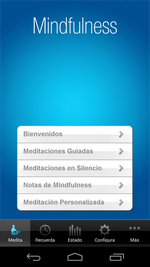
\includegraphics[width=0.19\textwidth]{figures/TMFA_main_section_screenshot_thumb.png}
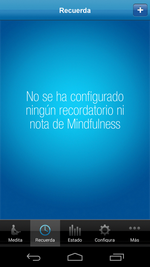
\includegraphics[width=0.19\textwidth]{figures/TMFA_reminder_section_screenshot_thumb.png}
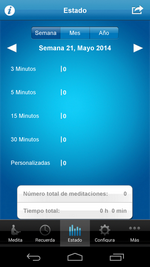
\includegraphics[width=0.19\textwidth]{figures/TMFA_stats_section_screenshot_thumb.png}
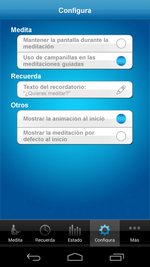
\includegraphics[width=0.19\textwidth]{figures/TMFA_config_section_screenshot_thumb.png}
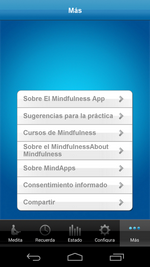
\includegraphics[width=0.19\textwidth]{figures/TMFA_more_section_screenshot_thumb.png}
\caption{Appearance of the five sections of The Mindfulness App.}
\label{fig:allScreens}
\end{figure}


In the following, we will describe in detail the functionalities and structure of each one of the sections.
\begin{itemize}
\item \textbf{Main/Meditation section:} The leftmost screen in figure \ref{fig:notes_screen_TMFA} shows the meditation section (which it has been chosen to be the main section) of the application. As it can be seen, the main section displays a menu in which five different options can be chosen: 
\begin{itemize}
\item \textit{Welcome:} This section shows a welcome message CHECK THIS AGAIN.
\item \textit{Guided Meditations}: This section offers 4 guided meditations of different durations (3, 5, 15, and 30 minutes).
\item \textit{Silent Meditations:} This section offers 4 silent meditations with bells of different durations (3, 5, 15, and 30 minutes).
\item \textit{Mindfulness notes}: This section contains a series of notes containing mindfulness related messages. This notes can be configured to be shown to the user at a given time or at a given place. The notes that are shown are either random or user-selected. Additionally, the user can create his own notes. The three rightmost screenshots in figure \ref{fig:notes_screen_TMFA} show the appearance of the Mindfulness notes section.
\item \textit{Personalized Meditations:} This section allows the user to create his own meditations. The options to customize the meditation are scarce. The application only allows to include/remove the guided introduction, to select the duration of the silent meditation and the time interval of the bells. Figure \ref{fig:personalized_meditation_TMFA} shows the appearance of the Personalized Meditations section. 
\end{itemize}


\begin{figure}[H]
\centering
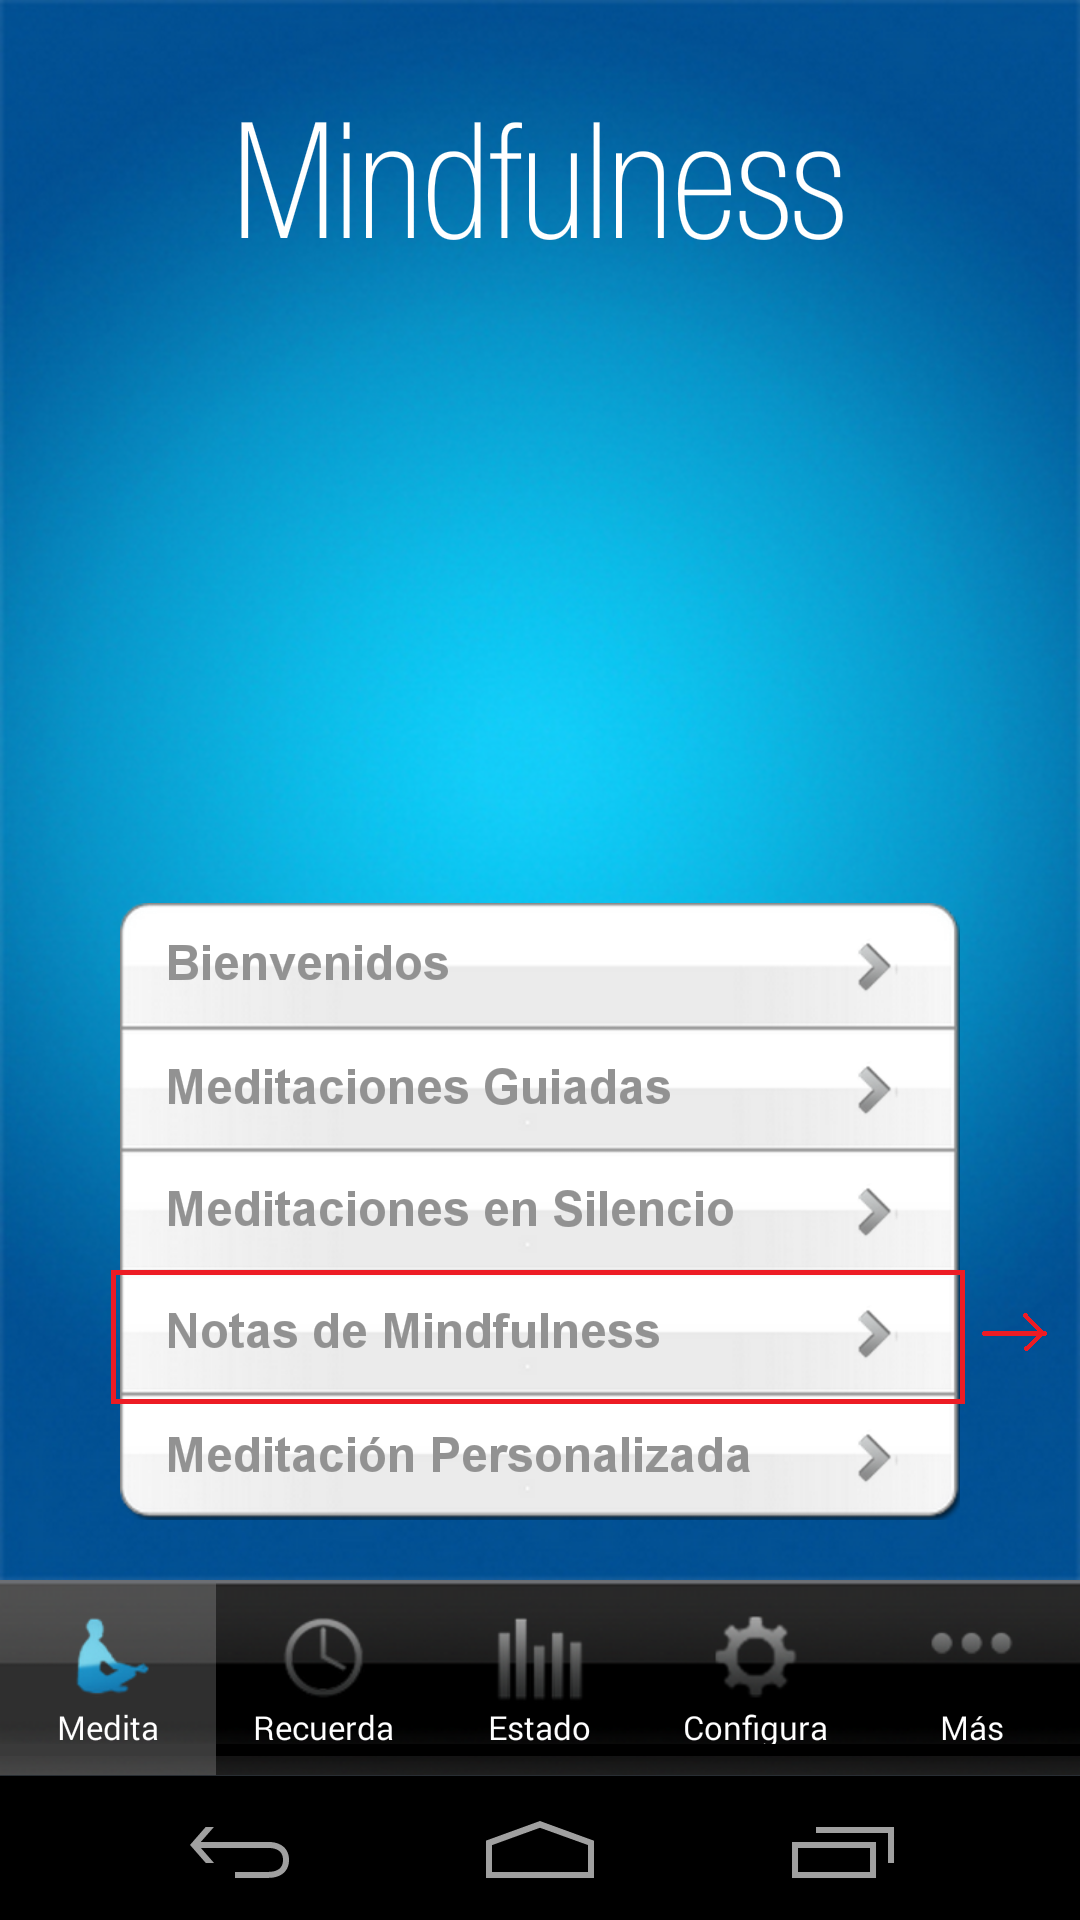
\includegraphics[width=0.20\textwidth]{figures/TMFA_main_section_screenshot_notes_arrow.png}
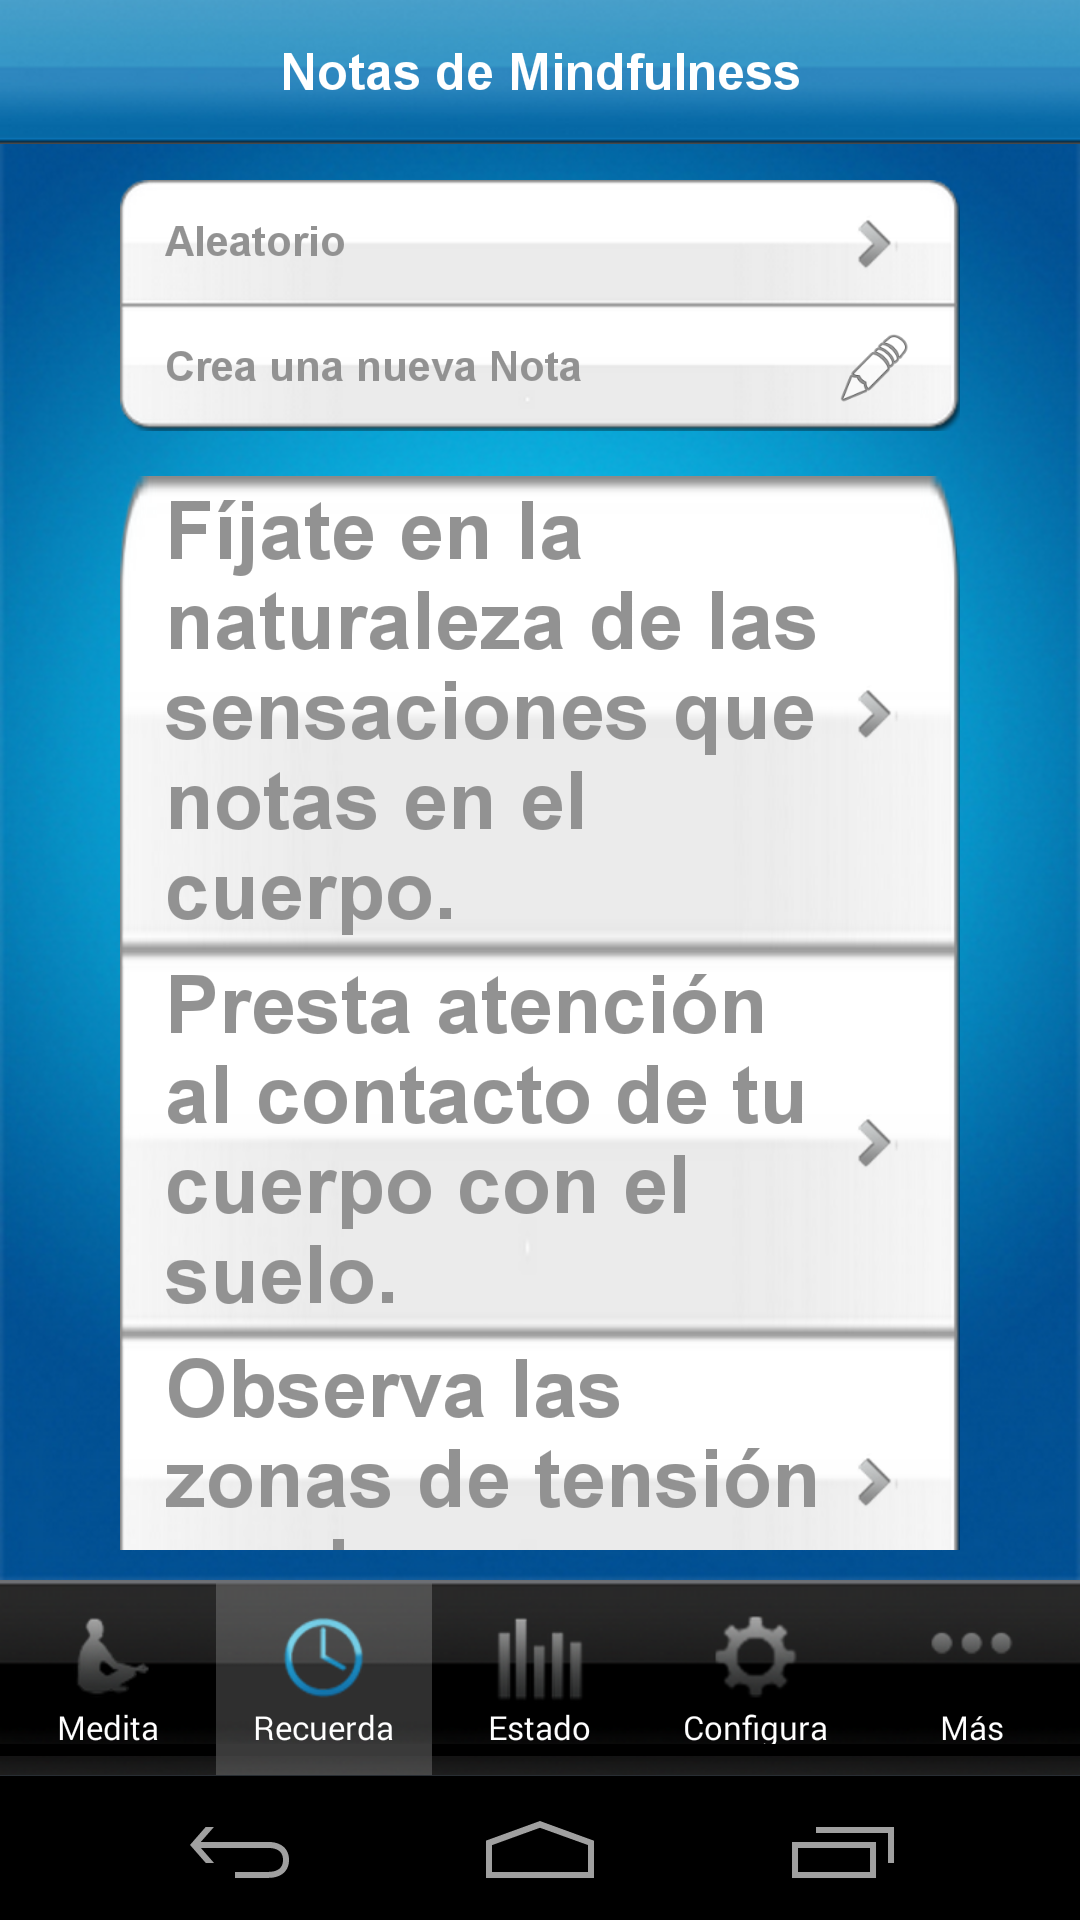
\includegraphics[width=0.20\textwidth]{figures/TMFA_notes_section_screenshot1.png}
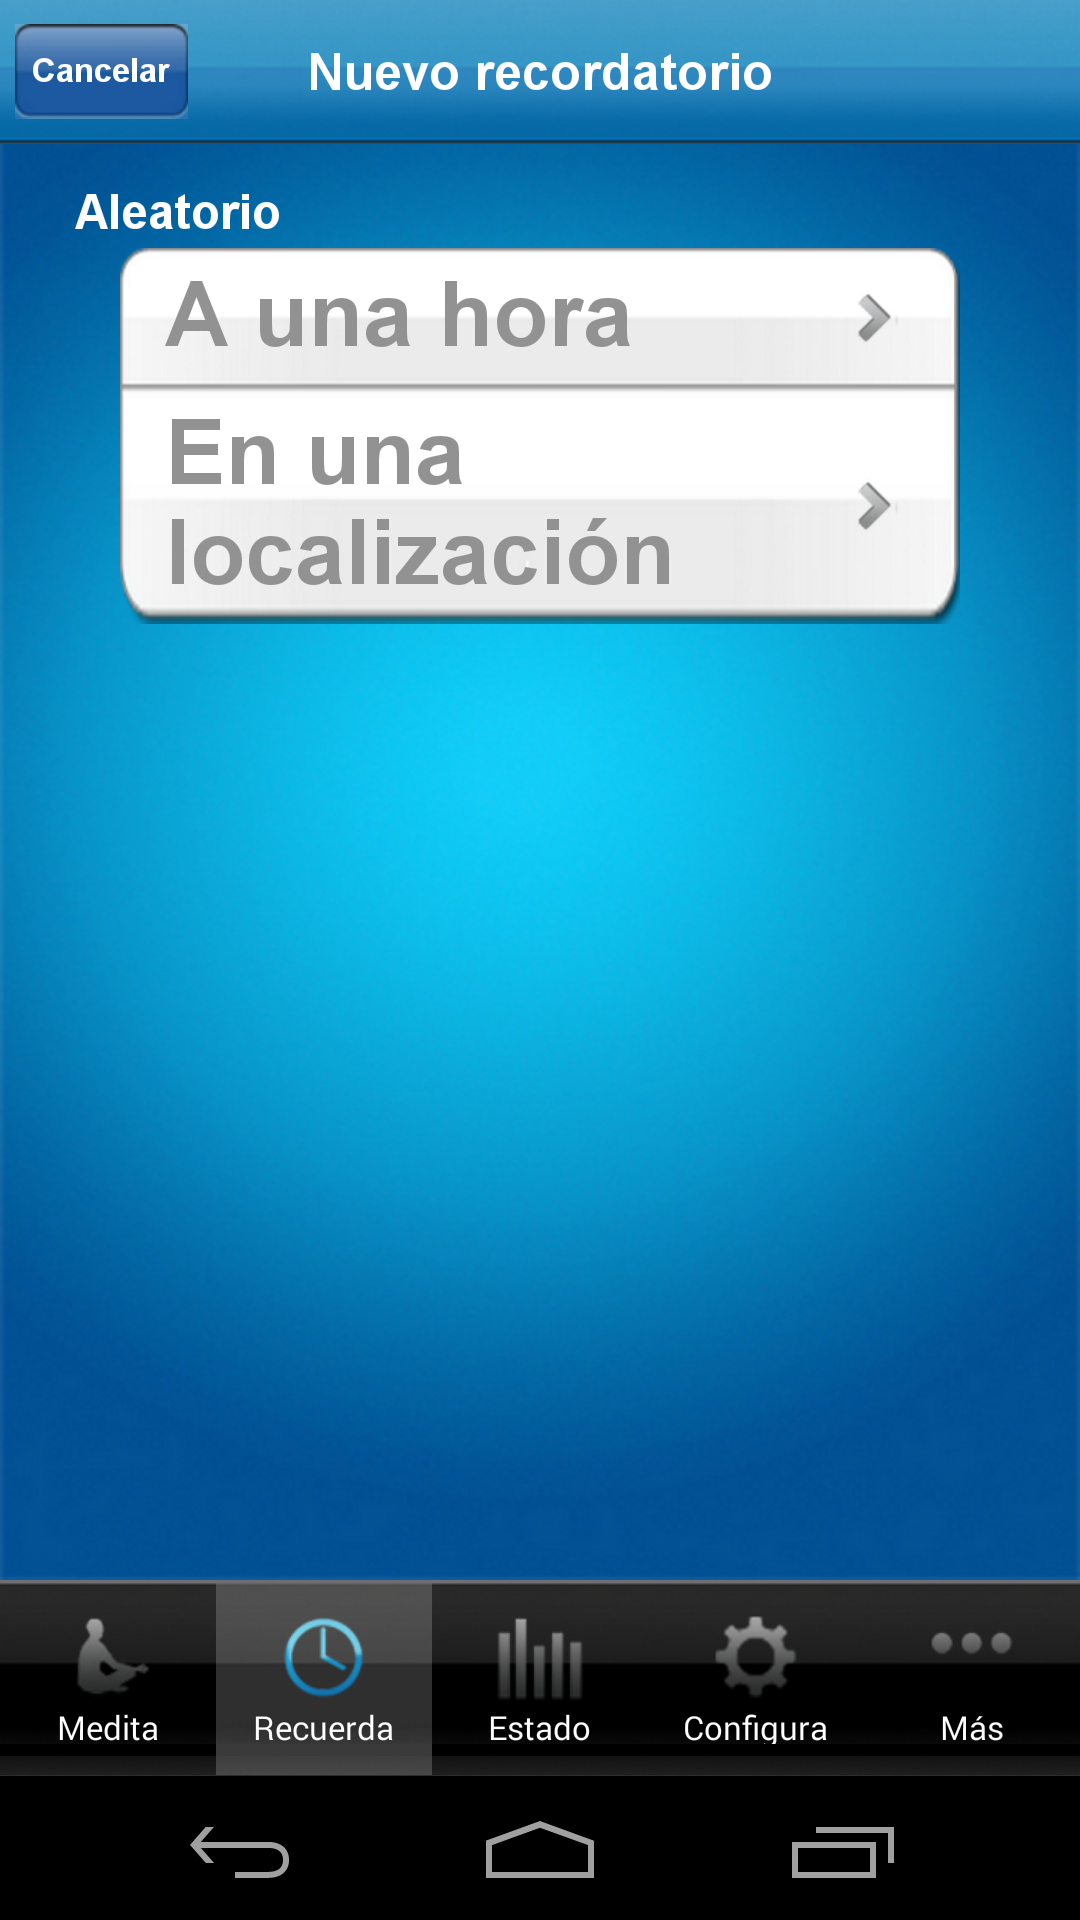
\includegraphics[width=0.20\textwidth]{figures/TMFA_notes_section_screenshot2.png}
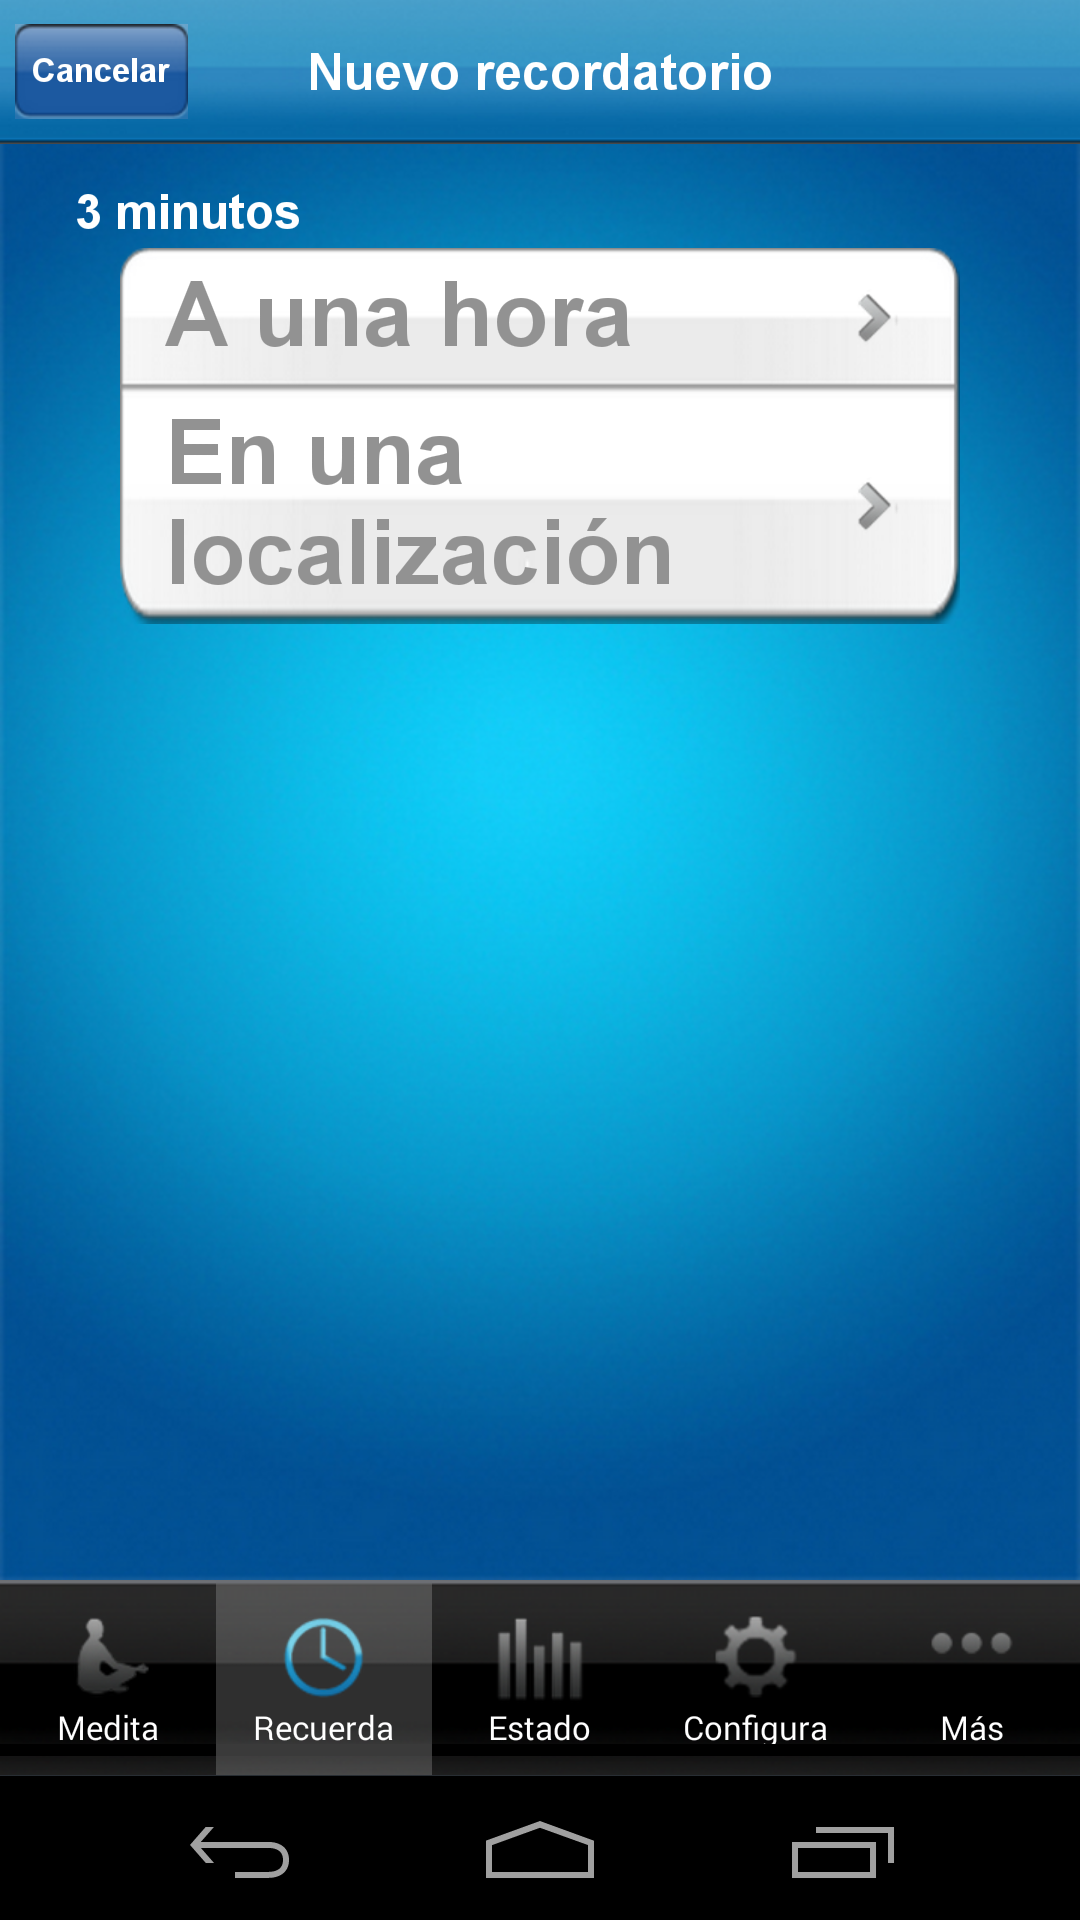
\includegraphics[width=0.20\textwidth]{figures/TMFA_notes_section_screenshot3.png}
\caption{Appearance of the Mindfulness notes section of The Mindfulness App.}
\label{fig:notes_screen_TMFA}
\end{figure}

\begin{figure}[H]
\centering
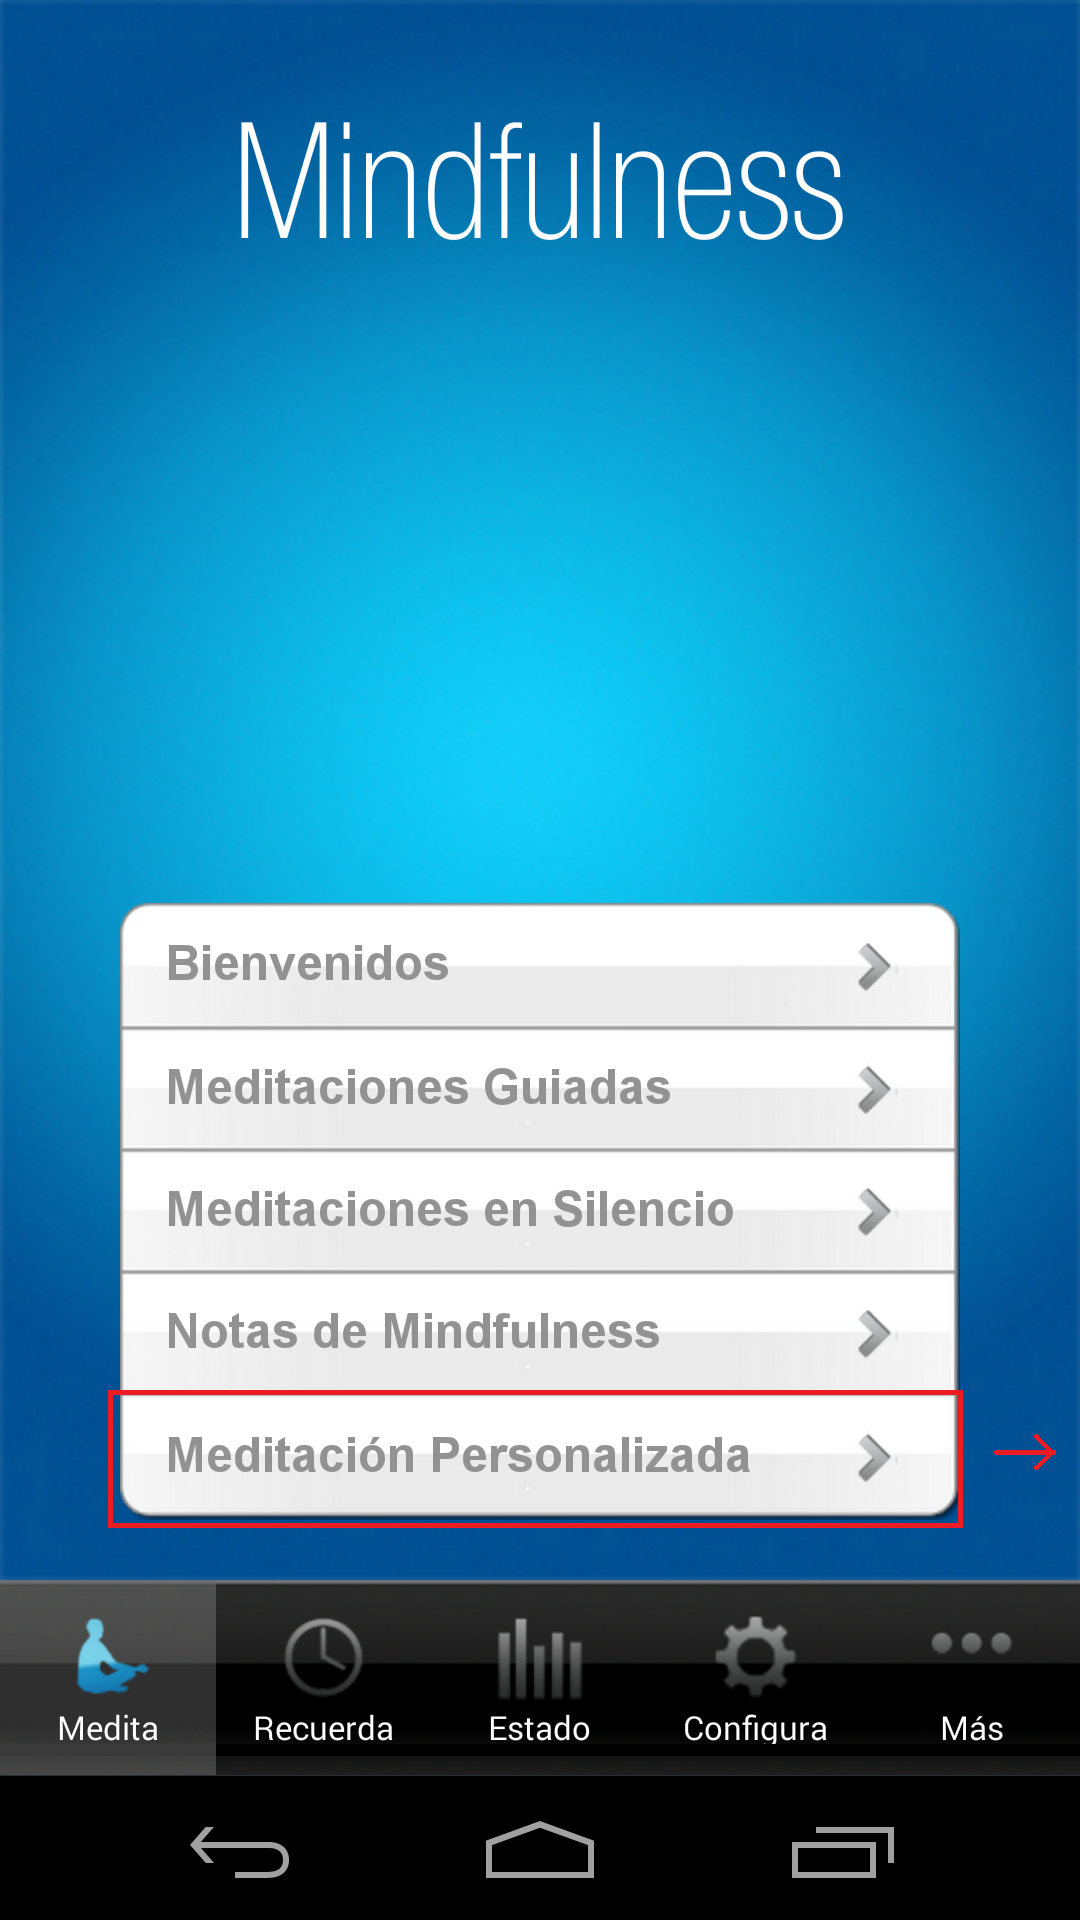
\includegraphics[width=0.20\textwidth]{figures/TMFA_main_section_screenshot_perso_arrow.png}
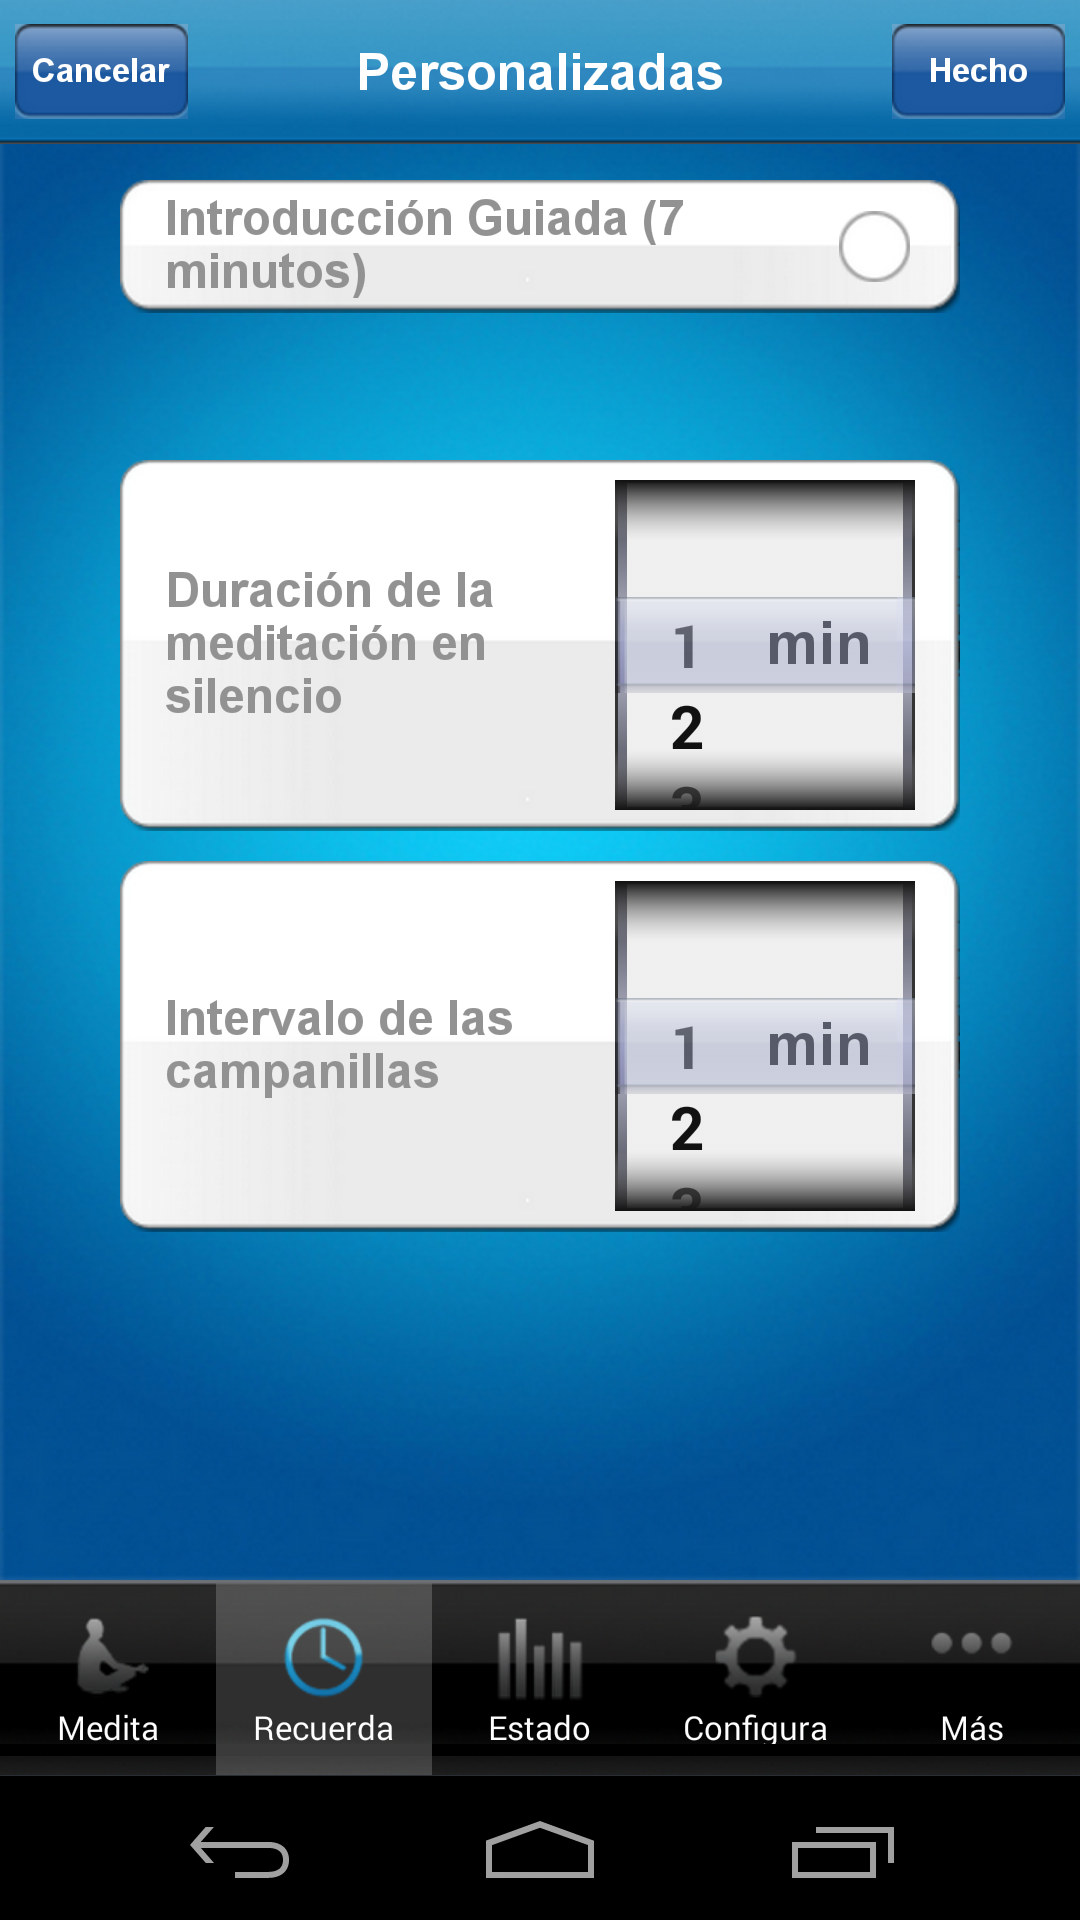
\includegraphics[width=0.20\textwidth]{figures/TMFA_perso_med_section_screenshot.png}
\caption{Appearance of the Personalized Meditations section.}
\label{fig:personalized_meditation_TMFA}
\end{figure}

\item \textbf{Reminders Section:} The user can set reminders to start a meditation or to pop up mindfulness notes. COMPLETE THIS. 
\item \textbf{Statistics Section:} This section contains statistics about the number of meditations. It basically shows the number of times per week, month and year, that a specific meditation was carried out.
\item \textbf{Configuration Section:} This section offers a few options to modify some aspects of some sections of the application. The options are listed below:
\begin{itemize}
\item Keep screen during meditation (YES/NO).
\item Use of bells during guided meditations (YES/NO).
\item Text of the reminders (Configurable by user).
\item Show animation at start-up (YES/NO).
\item Show default animation at start-up (YES/NO).
\end{itemize}
\item \textbf{More Section:} This section contains the following subsections:
\begin{itemize}
\item About The Mindfulness App: This section contains information about the application, its developers, its purpose and the person in charge of the traslation.
\item Suggestions of use: COMPLETE THIS.
\item Mindfulness Courses: COMPLETE THIS.
\item About Mindapps: This section contains information about the company which has developed the app.
\item Informed consent: COMPLETE THIS.
\item Share: COMPLETE THIS.
\end{itemize}

Figure \ref{fig:reminders_stats_config_more_TMFA} shows screenshots of the \textit{reminders}, \textit{statistics}, \textit{configuration} and \textit{more} sections.
\begin{figure}[H]
\centering
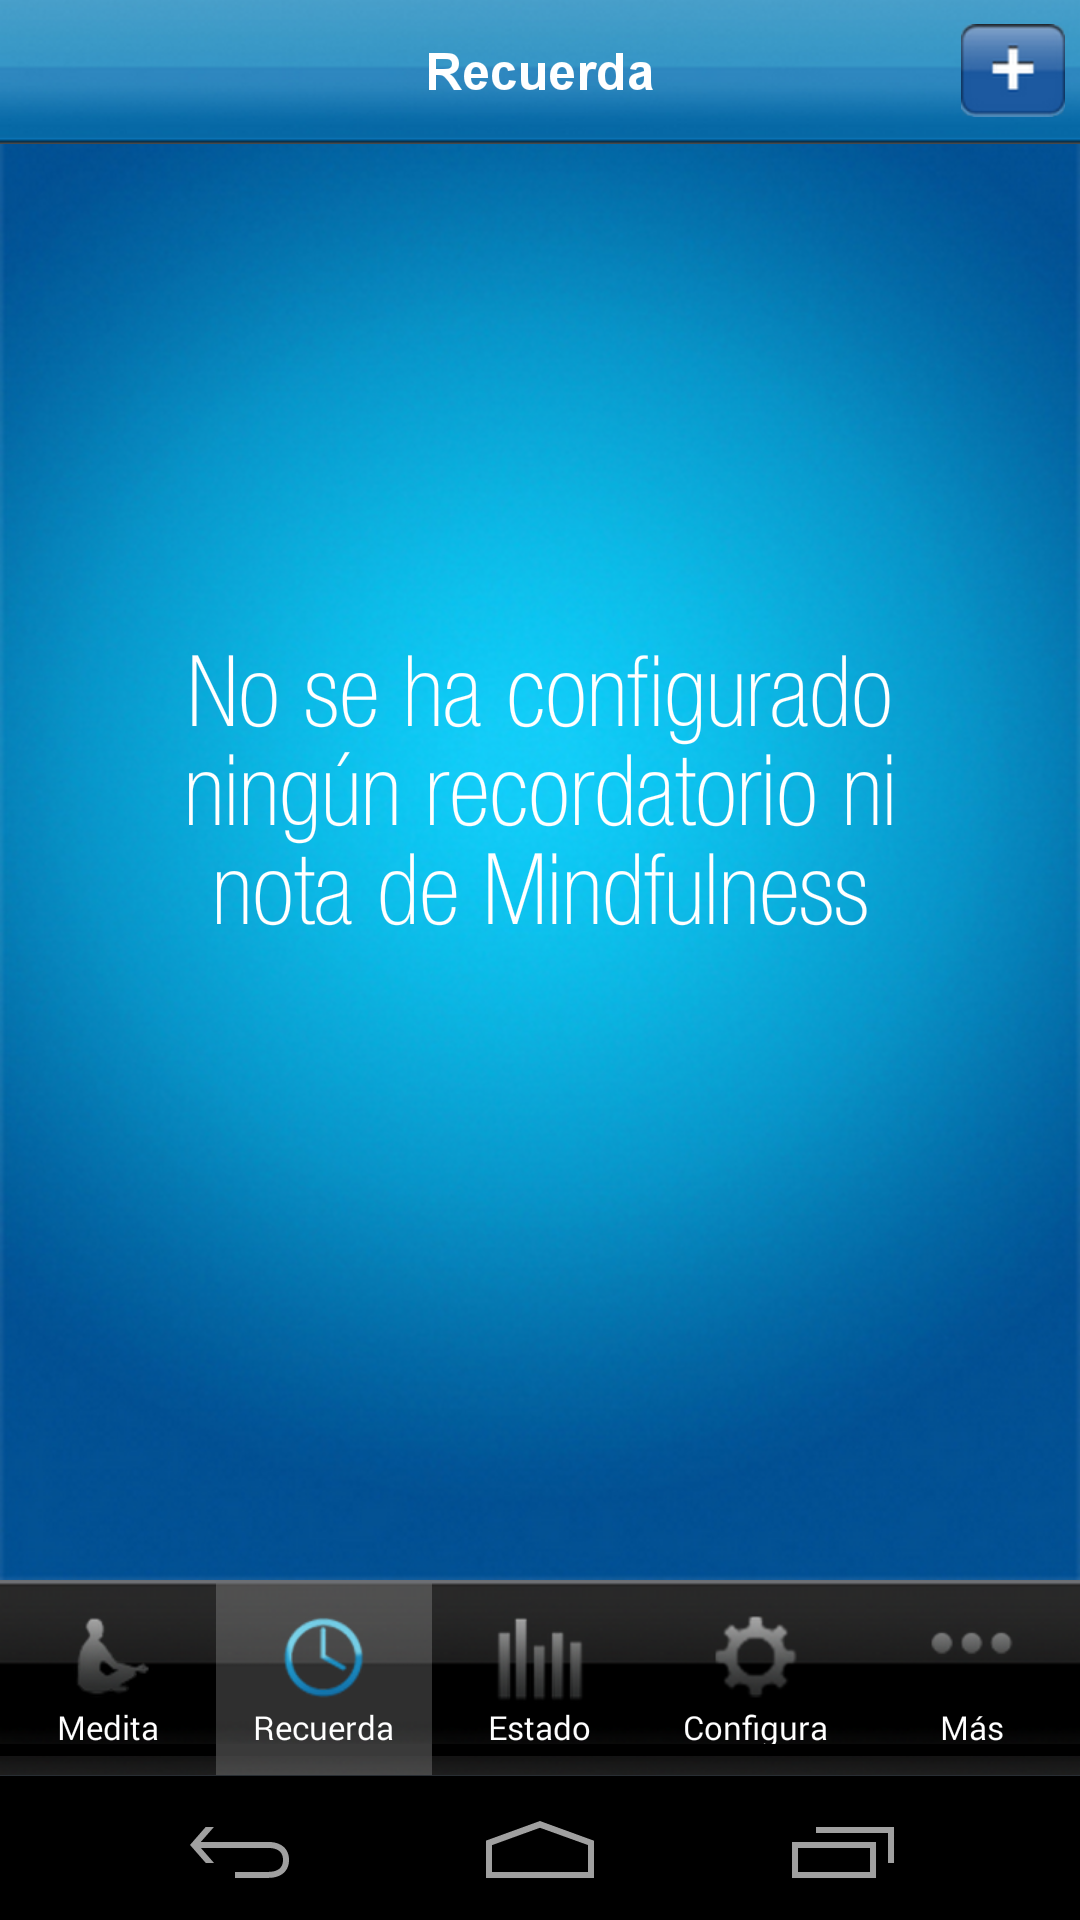
\includegraphics[width=0.20\textwidth]{figures/TMFA_reminder_section_screenshot.png}
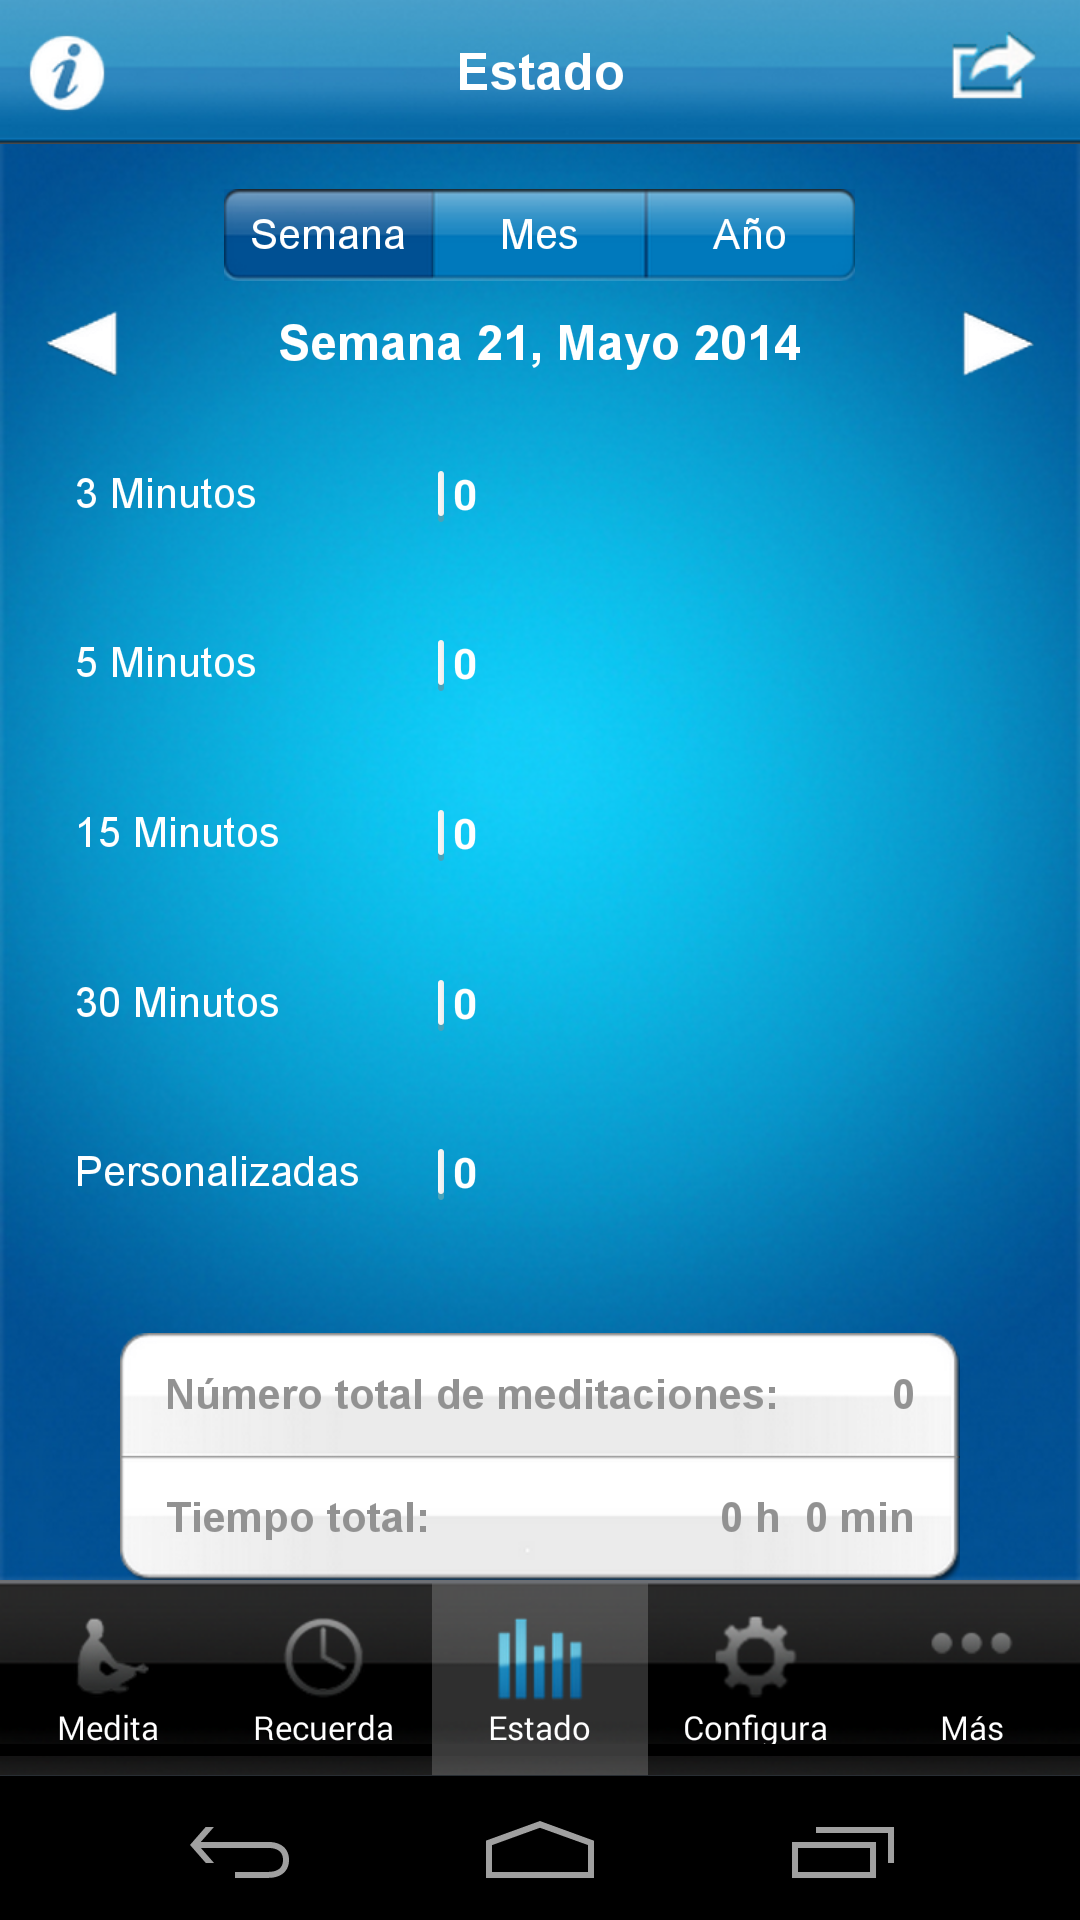
\includegraphics[width=0.20\textwidth]{figures/TMFA_stats_section_screenshot.png}
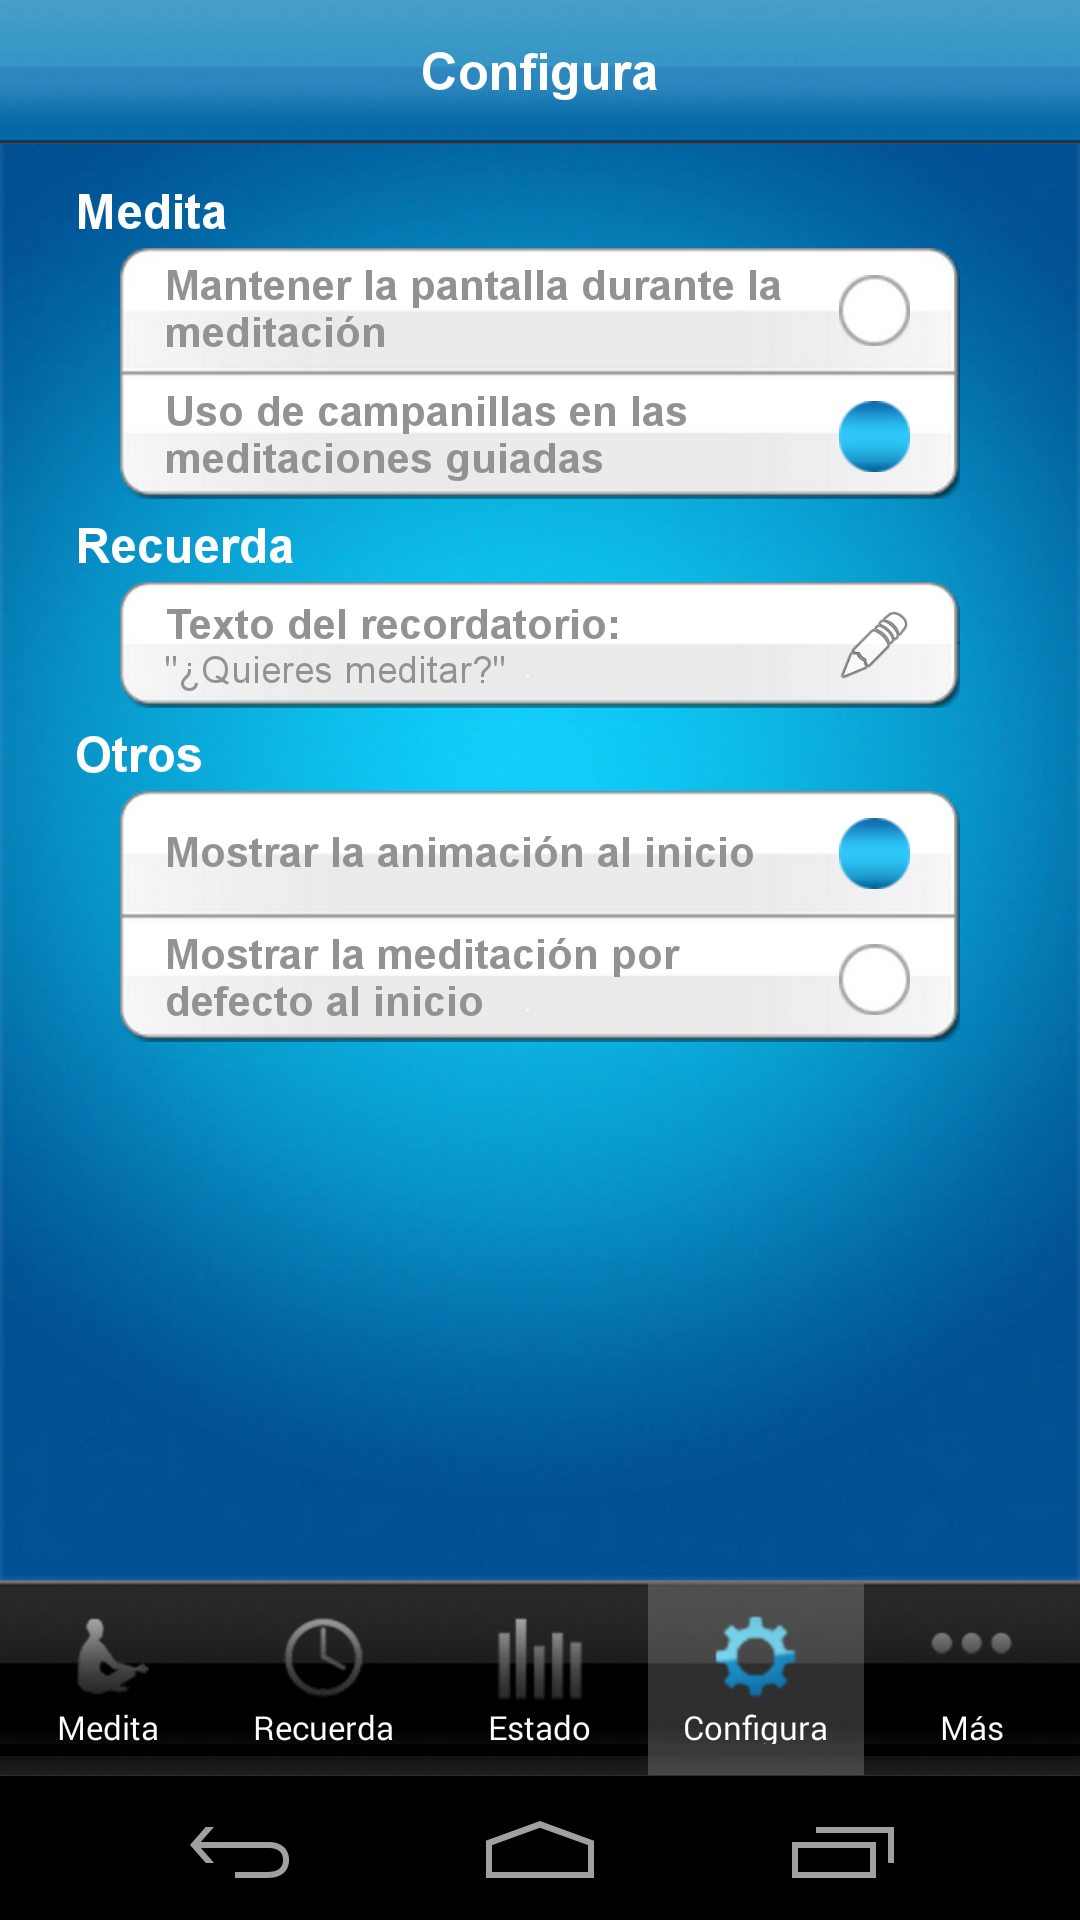
\includegraphics[width=0.20\textwidth]{figures/TMFA_config_section_screenshot.png}
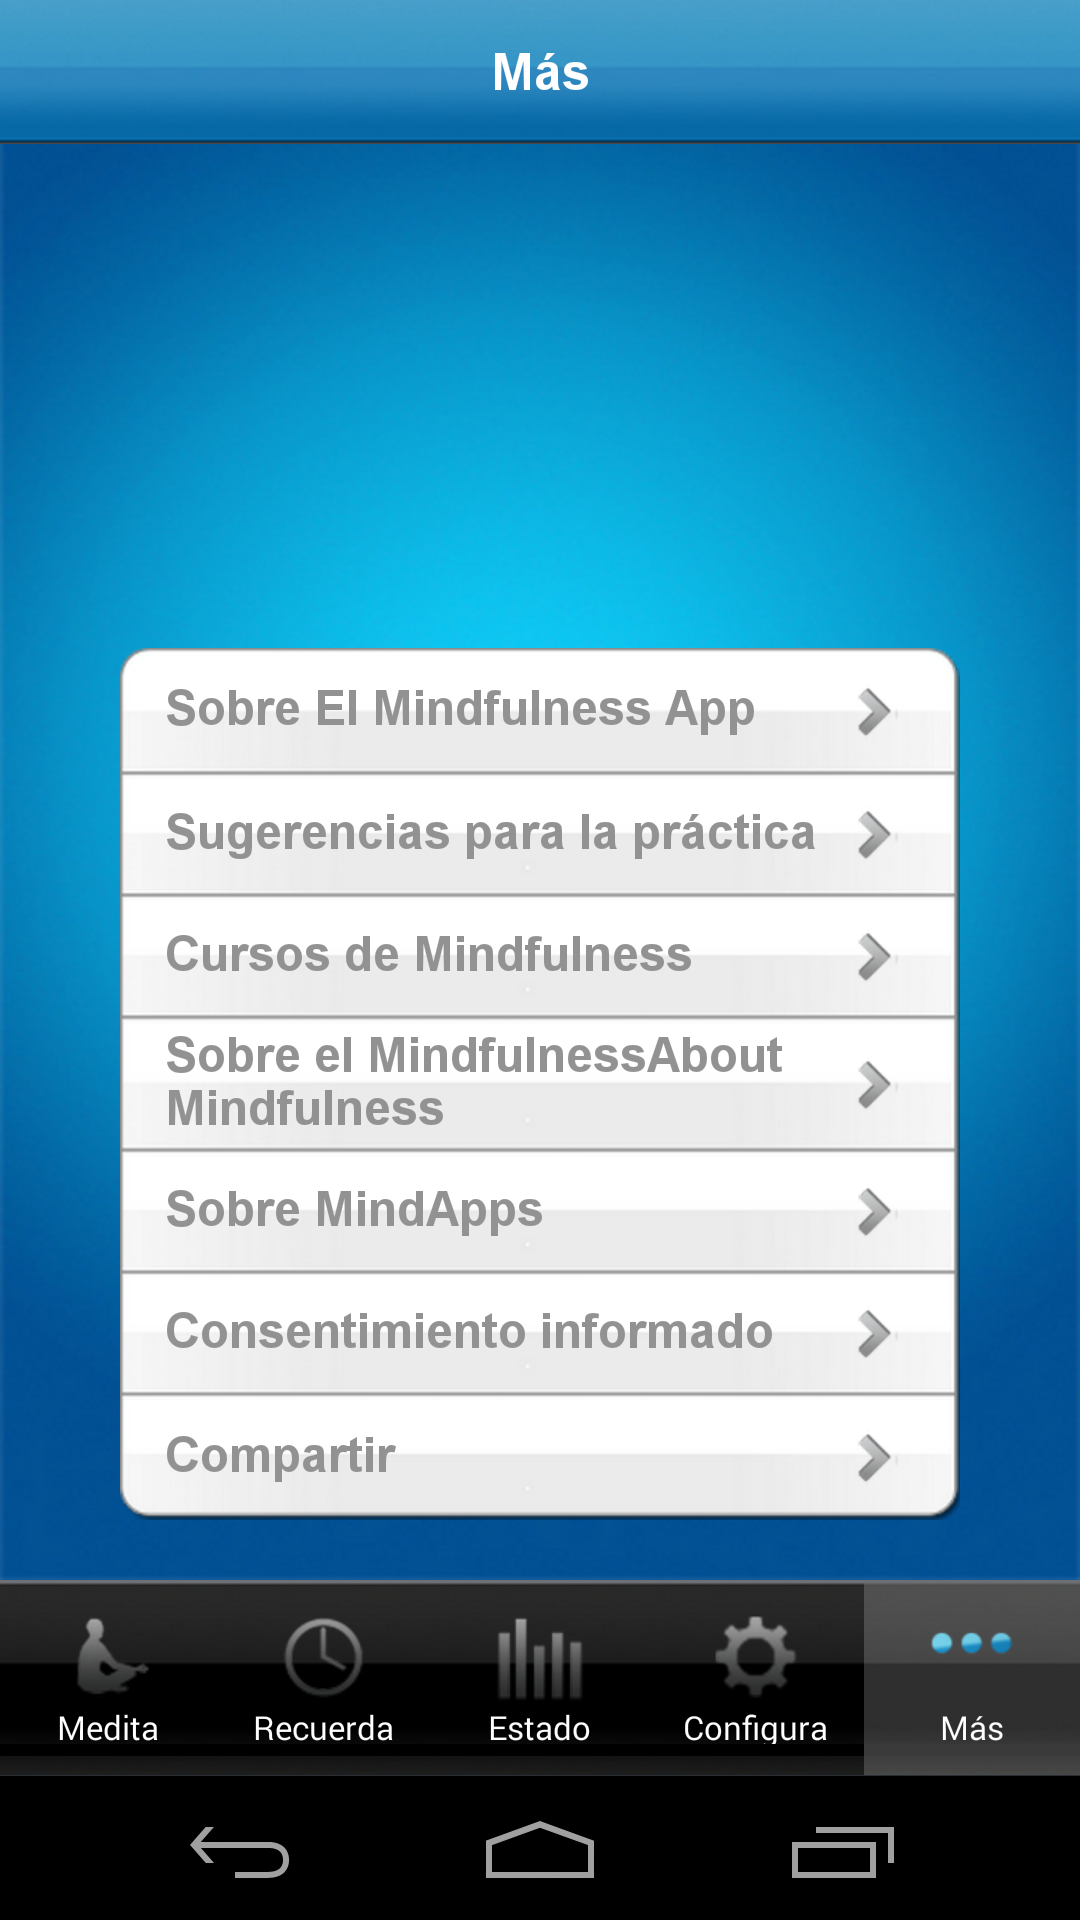
\includegraphics[width=0.20\textwidth]{figures/TMFA_more_section_screenshot.png}
\caption{Appearance of the reminders (left), statistics (center-left), configuration (center-right) and more (right) sections.}
\label{fig:reminders_stats_config_more_TMFA}
\end{figure}

\end{itemize}
\subsubsection{Analysis of content}
TO BE COMPLETED WHEN GONZALO COMES BACK.

\subsubsection{Analysis of business model and strategy}
The business model for the Android app is different from the iOS app. For the Android app the only revenue stream is the price payed to download it. Therefore, it follows a pay-once strategy and obtains no extra value from customers who use the application. \\
\indent On the other hand, in addition to the pay-once strategy, the iOS app includes a store which permits the user to buy and download extra meditations which are designed by leading figures of the meditation scene. This allows the company to monetize users (as they may become returning customers) after they have downloaded the application and can also be helpful to increase their satisfaction and involvement in the platform. This strategy also supposes the creation of a basic multi-sided platform \footnote{Two-sided markets, also called two-sided networks, are economic platforms having two distinct user groups that provide each other with network benefits. The organization that creates value primarily by enabling direct interactions between two (or more) distinct types of affiliated customers is called multi-sided platform (MSP).} as the application is a small-sized platform which establishes contact between meditators and creators of medidation routines. 
\subsubsection{Critical Analysis}
This is arguably the best MBMA in the market and still it has many things that could be improved.
\begin{itemize}
\item \textbf{Navigation and interface}: The navigation is not always clear and there are many redundant options which can be accessed from different screens, which is sometimes a bit confusing.
\item \textbf{Graphic design}: The graphic design is very improvable. The fonts are too large, and the gray boxes which contain the submenus are not fancy.
\item \textbf{Content}: 
\end{itemize}

\subsubsection{Users' feedback}

\begin{itemize}
\item \textbf{Android}: The users make very positive comments about the application. They state that the application is intuitive, easy to use and very good to take up into meditation. Some of the users suggest to include a clock sound (tic-tac) as one of the background sounds of the meditations. One of the users says that he downloaded the application because it was recommended in a mindfulness course he followed. 

\item \textbf{iOS}: There are only three reviews by users so we will directly reproduce them here.
\begin{itemize}
\item \textit{Once I got over the fact that the woman guiding the meditation kept using impersonal terms like "what is the state of mind" instead of "what is your state of mind," I found the voice very calming. As someone who experiences palpitations at night, this seems to help by taking my whole level of anxiety down a notch and giving me some breathing procedures and ways of thinking that I can use when I have a palpitation episode. It doesn't always help, but sometimes it does and that's worth something. Interesting how my perception of the amount of time between her comments can vary so much from day to day."}
\item \textit{"I have recently completed Jon Kabat-Zinn's Mindfulness Based Stress Reduction class and have found this app to be better than the class CDs because of its versatility. I had been worried I would not be able to maintain my meditation practice but this app is keeping me on track. It can be stressful to fit stress reduction into your life style! This app alleviates a little of that stress with reminders and by the features that let you customize each meditation."}
\item \textit{"It is a great app to help you maintain a routine of at least a few minutes of daily meditation. The options are great, but I would love to be able to set how often the bells should ring during silent meditation and to have a few options of voices for the guided meditations. I recommend and gift this app for all those who enjoy or are starting a life practicing meditation!".}
\end{itemize}
\end{itemize}
\subsubsection{Wrap-up}
HERE GOES THE WRAP-UP HERE GOES THE WRAP-UP HERE GOES THE WRAP-UP HERE GOES THE WRAP-UP HERE GOES THE WRAP-UP HERE GOES THE WRAP-UP HERE GOES THE WRAP-UP HERE GOES THE WRAP-UP
\begin{table}
\centering
\begin{tabular}[!h]{|l|l|}
\hline
\textbf{Operating System} & iOS 6 or later and Android 2.2 or later. \\ \hline
\textbf{Price} &  \euro{1.74} (Android) and \euro{1.78} (iOS)\\ \hline
\textbf{Revenue stream} & Pay once (Android), Pay once and extra premium content (iOS)\\ \hline 
\textbf{Number of downloads} & $10,000 - 50,000$ (Android) and $\sim70,000$ (iOS).\\ \hline
\textbf{Users' rating} & 4.2 out of 5 (English version), 4.8 out of 5 (Spanish version).\\ \hline
\textbf{Content} &	\\ \hline
\textbf{Functionalities}& \\ \hline

\end{tabular}
\end{table}

%--------------------------------------------------------------
%			SIMPLY BEING
%--------------------------------------------------------------

\subsection{Simply Being}
\begin{wrapfigure}{l}{0.08\textwidth}
  \vspace*{-0.8cm}
  \begin{center}
    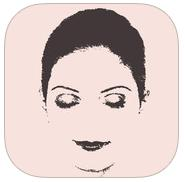
\includegraphics[width=0.08\textwidth]{figures/SB_icon.jpg}
  \end{center}
  \vspace*{-0.5cm}
\end{wrapfigure}
Simply Being is a guided meditation application, offered by Meditation Oasis, a webpage created by Mary and Richard Maddux. Mary is a meditation instructor and Richard is a music composer specialized in meditation, relaxation and healing. The application is offered under a payment of \euro{0,73} for Android and \euro{0,89} for iOS. It has been downloaded  $10.000 - 50.000$ (est. $29.000$) times from the Play Store and around $73.000$ times from the AppStore (estimated by xyo.net). The Android version was last updated on Dec 19 2013, and the iOS version on Jul 1 2013.\\

This application offers a very simple and straightforward way for users to do guided meditations, letting them select a background sound or music and the duration of the exercise. The design is plain, a background image and transparent buttons. The differences between the iOS and the Android versions are minimal, only some visual changes on the menus, based on the native interface of each OS. \\

The application is not localized, being offered only in the English language. 

\subsubsection{Features} 

According to the developer, these are the main functionalities of their application:
\begin{itemize}
\item Meditate easily as you are voice-guided step by step.
\item Choose a meditation length of 5, 10, 15 or 20 minutes.
\item Listen to the meditation with or without music/nature sounds.
\item Listen to the music or nature sounds alone.
\item Read instructions to support and enhance your meditation.
\item Relax deeply and experience the present moment completely.
\item Enjoy the benefits of meditation.
\item Links to support on the Meditation Oasis website.
\item Separate Volume Controls for voice and music/nature sounds.
\end{itemize}

As we can see this app doesn't offer a lot of fancy features, but for the user expecting to use is as a tool for guided meditation is enough. Some of the "features" announced are not really so, but supposed effects of its use. 

\subsubsection{Analysis of the user interface}

We will analyze the Android application, which is the one we have access to. The interface has the same background for every section, a subtle drawing of a tree and a starry night in a emerald green tone, with the name of the app on the top. There is no other menu, or ways to go from one section to another apart from going back to the start menu. Each section has a "Menu" button on the bottom of the screen to go back to the start menu. \\

In figure \ref{fig:SB_allScreens} all the sections are shown except the guided meditation, which will be analyzed later. 

\begin{figure}[H]
\centering
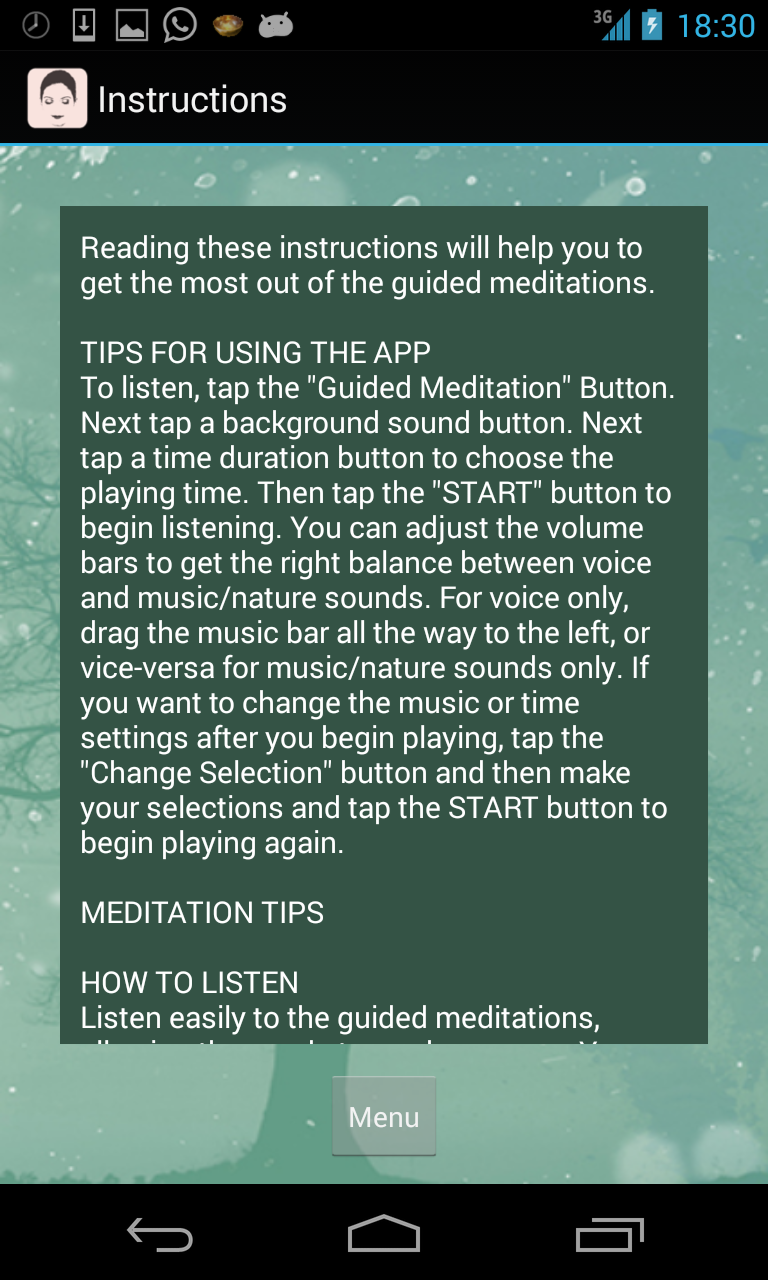
\includegraphics[width=0.32\textwidth]{figures/SB_instructions.png}
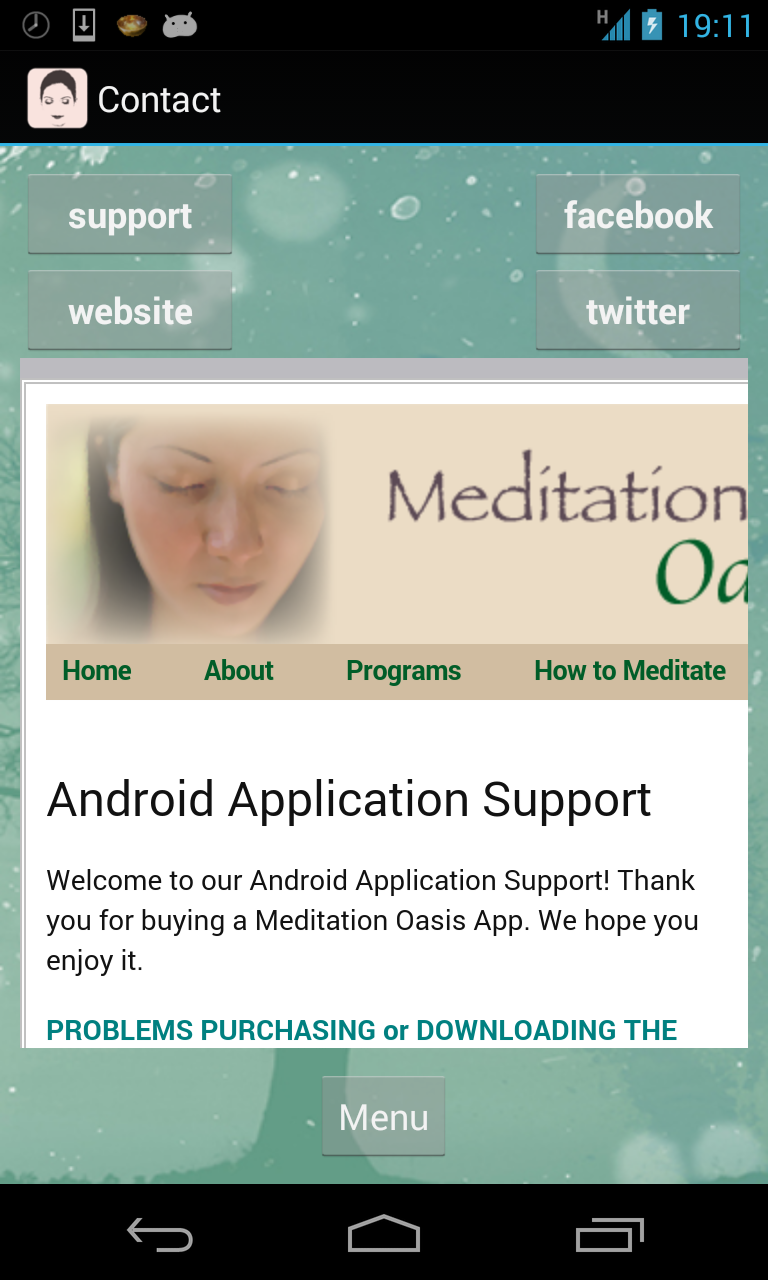
\includegraphics[width=0.32\textwidth]{figures/SB_contact_screenshot.png}
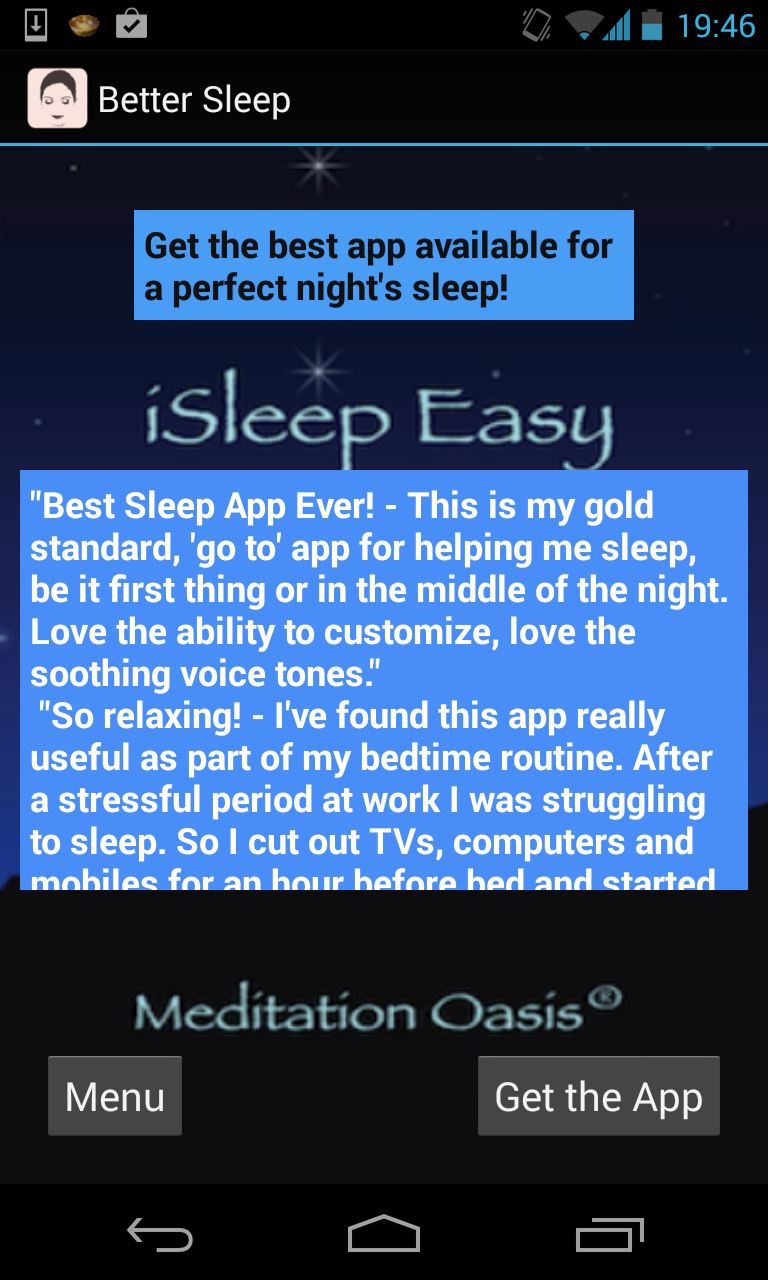
\includegraphics[width=0.32\textwidth]{figures/SB_promotion.png}
\caption{Appearance of the secondary sections of the Simply Being application.}
\label{fig:SB_allScreens}
\end{figure}

First we will analyze each of the secondary sections.

\begin{itemize}
\item \textbf{App Instructions:} This section shows a scrollable frame of text that covers most of the screen, containing some guidance on the use of the application and general tips on meditation. The frame has a solid background that is not in line with the look of the rest of the application. 
\item \textbf{Contact:} This section contains four buttons at the top which lead to the website and social profiles of the content creators. The rest of the screen (saving the bottom "Menu" button) is a \textit{WebView} frame containing the Android Application Support page. The look is very poor, since the web page shown is not optimised for the resolution of the frame and the user can scroll vertically and horizontally through it. Also, any link clicked inside the frame will open in the predefined browser, thus leaving the application. 
\item \textbf{Rate This App:} This is just a link to the Google Play page of the application.
\item \textbf{Better Sleep:} This section is just a promotion for another application of the same creators. It uses another background that breaks completely the style of the application. The text background is a solid blue that is also not in line with the rest of the application.
\end{itemize}

Now we will analyze the main section, which is the Guided Meditation.

\begin{figure}[H]
\centering
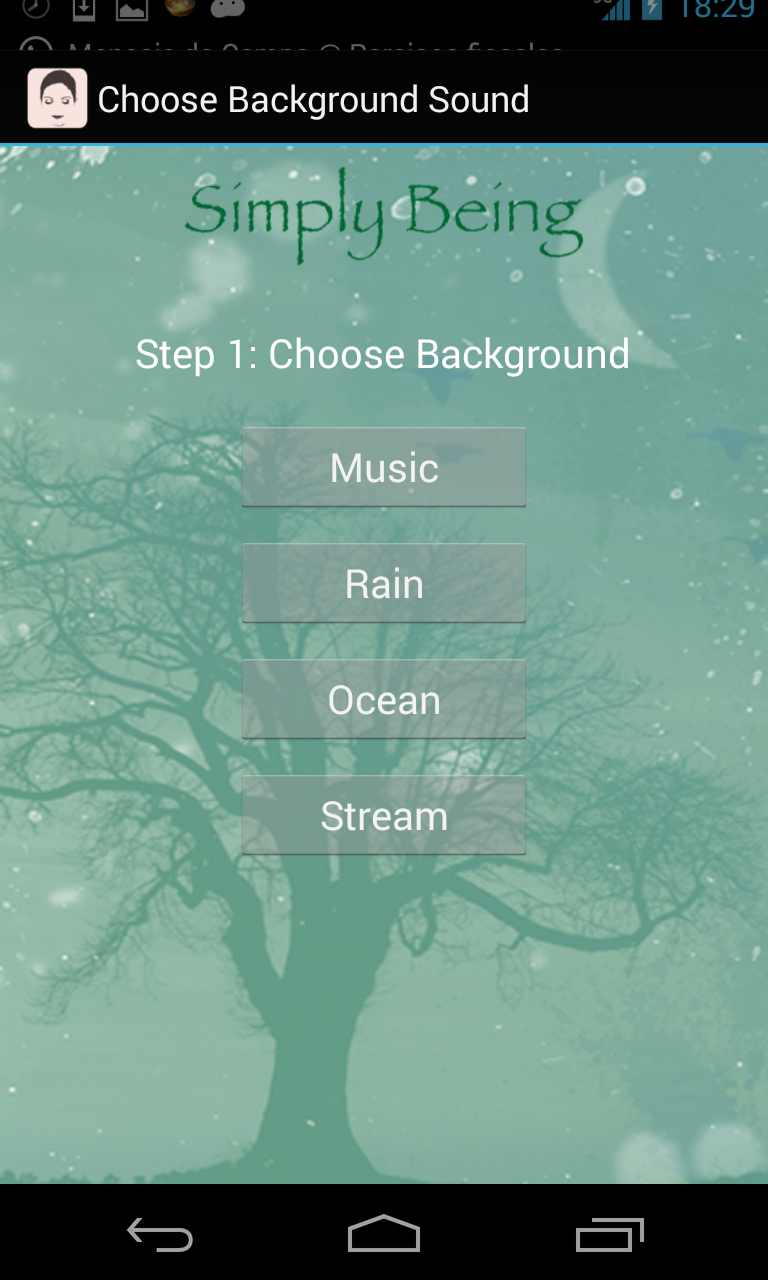
\includegraphics[width=0.24\textwidth]{figures/SB_choose_background_screenshot.png}
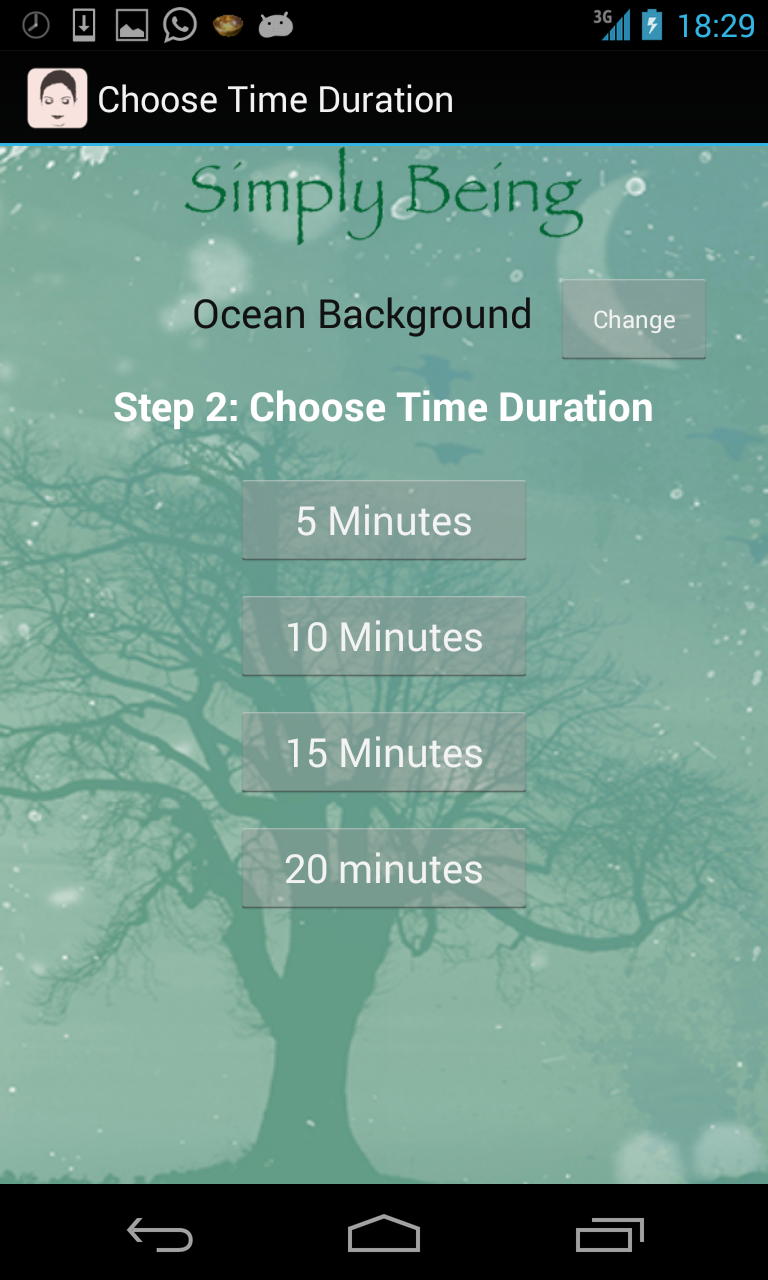
\includegraphics[width=0.24\textwidth]{figures/SB_choose_duration_screenshot.png}
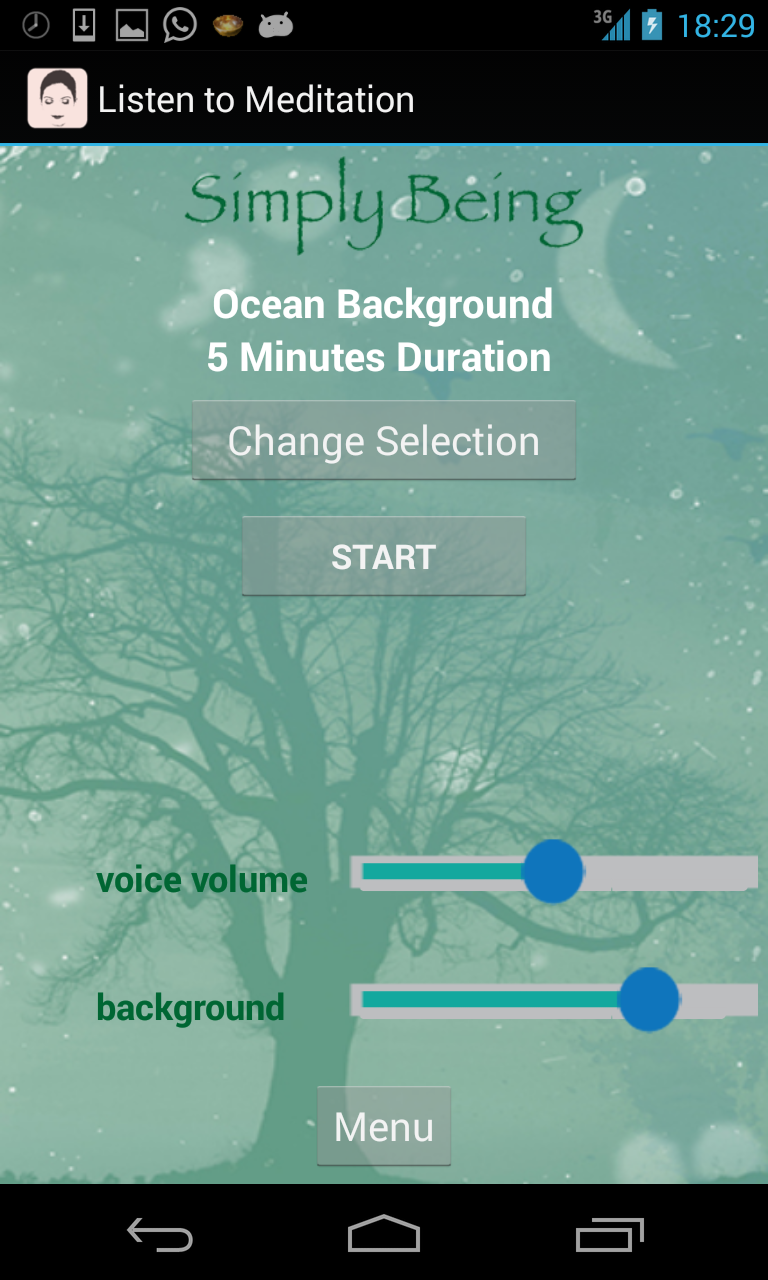
\includegraphics[width=0.24\textwidth]{figures/SB_start_meditation_screenshot.png}
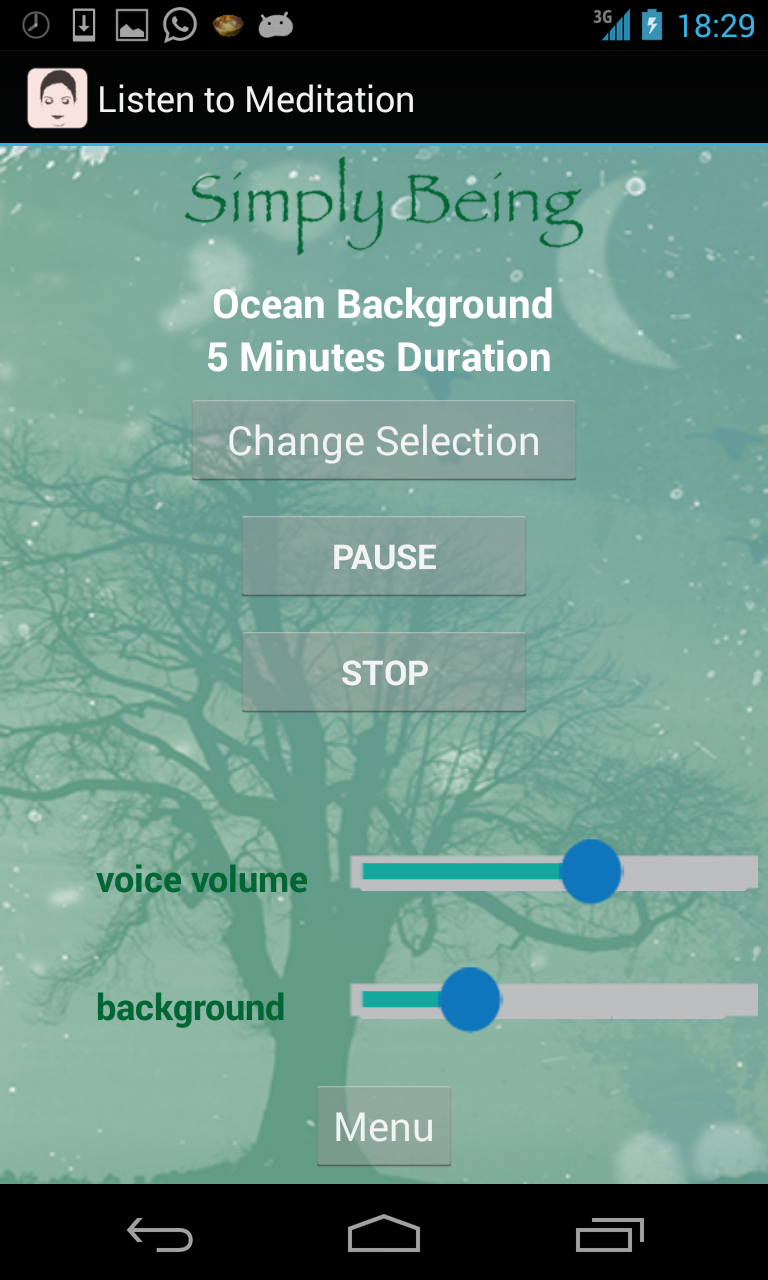
\includegraphics[width=0.24\textwidth]{figures/SB_during_meditation_screenshot.png}
\caption{Appearance of the Guided Meditation process in the Simply Being application.}
\label{fig:SB_meditation}
\end{figure}

When we select the Guided Meditation option, we are presented with four options of background sounds:

\begin{itemize}
\item Music.
\item Rain.
\item Ocean.
\item Stream.
\end{itemize}

The next step lets you choose the duration of the meditation:

\begin{itemize}
\item 5 Minutes.
\item 10 Minutes.
\item 15 Minutes.
\item 20 Minutes.
\end{itemize}

A good design decision on this step is showing at the top the background selection you have just made, and letting you change it if wanted. \\

After choosing background and duration the meditation screen is presented. At the top, both choices are shown, with a button that lets you change them. Below this the play button lets you start the meditation. At the bottom of the screen, there are two sliders so the user can adjust the background and voice volume, and finally the button to go back to the main screen. When the start button is pressed, it is replaced by the pause, and another, stop button, appears. When paused, only a resume button is shown. \\

The app's navigation is intuitive and fast, but the device's back button is not well integrated. The user expects the back button to bring him to the last screen, but if he is already in the main menu the back button should exit the application and not go back to previous screens. There is no "exit" or "close app" button, so the only way to exit is to press the back button repeatedly until the stack of previous screens is empty and the next press does what is intended to do and exits.

\subsubsection{Analysis of content}
TO DO:TRY TO LISTEN TO THE MEDITATIONS

\subsubsection{Analysis of business model and strategy}

The only source of revenue for the creators comes from the cost of the application on the Google Play and iTunes stores. There are no in-app purchases available or extra content. The application feels more like a way for the creators to broaden their audience and make themselves better known. On their website, they offer paid meditation courses and other materials which are probably their main source of revenue. 

\subsubsection{Critical Analysis}
The application does what it is expected by the user, but the interface is poorly thought out, with inconsistencies between screens. Also the native buttons, even though they are transparent, make the application look cheap.\\

The content.... LISTEN TO THE MEDITATIONS

\subsubsection{Users' feedback}

On Google Play, the application has a 4.4 out of 5 rating with 370 total opinions, but not a single comment, which is strange given that it has been purchased at least over $10.000$ times. \\

On iTunes App Store, it has a 4.3 out of 5 rating (no info on the number of ratings).\\

Reading the comments on xyo.net for both iOS and Android versions, most users praise the application's simplicity of use. The content gets a lot of positive feedback too, because of the calm and soothing voice and the relaxing sounds and music. The only negative review finds the quantity of options lacking, and also criticises the impossibility to customize it in any way.


\subsubsection{Wrap-up}

This application shows that even paid apps have a market if they deliver what they announce, and there are people out there looking for meditation applications and willing to pay if the content has enough quality, even if the application itself is not very fancy looking. For most users the important part is the content and the ease of use, while there is a minority that looks for more options and customization.

%--------------------------------------------------------------
%         MINDFULNESS BELL
%--------------------------------------------------------------

\subsection{Mindfulness Bell}
\begin{wrapfigure}{l}{0.08\textwidth}
  \vspace*{-0.8cm}
  \begin{center}
    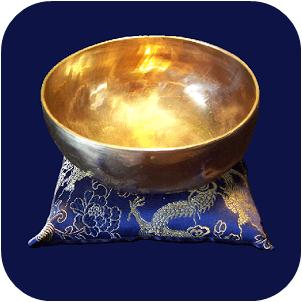
\includegraphics[width=0.08\textwidth]{figures/MB_icon.jpg}
  \end{center}
  \vspace*{-0.5cm}
\end{wrapfigure}
The Mindfulness Bell rings periodically during the day, to give you the opportunity to hold on for a moment and consider what you are currently doing, and in what state of mind you are while you are doing it. It is developed by Mindful Apps (no more info since their website http://www.mindful-apps.com/ is down). The application is offered for free, and it has been downloaded around $149.000$ times from the Play Store (est. by xyo.net). It was last updated on Jan 4 2012. There is an application with the same name in the Apple AppStore, but it is not developed by the same team (although the similarities are suspicious). \\

The application is as simple as it can be, it lets the user define the periodicity of the bell and it will sound during the day. The interface is minimal, since nothing more is needed. It is only available in English. 

\subsubsection{Features} 

The main functionalities of the application are:
\begin{itemize}
\item Bell sounds with variable intervals (from 5 minutes to 4 hours)
\item Define start and stop bell times (so it doesn't sound at night)
\item Various mute and vibrate options
\end{itemize}

The concept is simple and so is the application, it offers just what it is expected of it. 

\subsubsection{Analysis of the user interface}

When opened, the application shows a photo of a meditation bell with a text on the bottom that explains the purpose of the bell. There is a small menu button at the bottom bar that lets the user select between 'Settings' and 'About'. The bell sounds if the user taps the screen, and a small message pops up asking to use the menu button.  \\

In figure \ref{fig:MB_allScreens} all the screens are shown.

\begin{figure}[H]
\centering
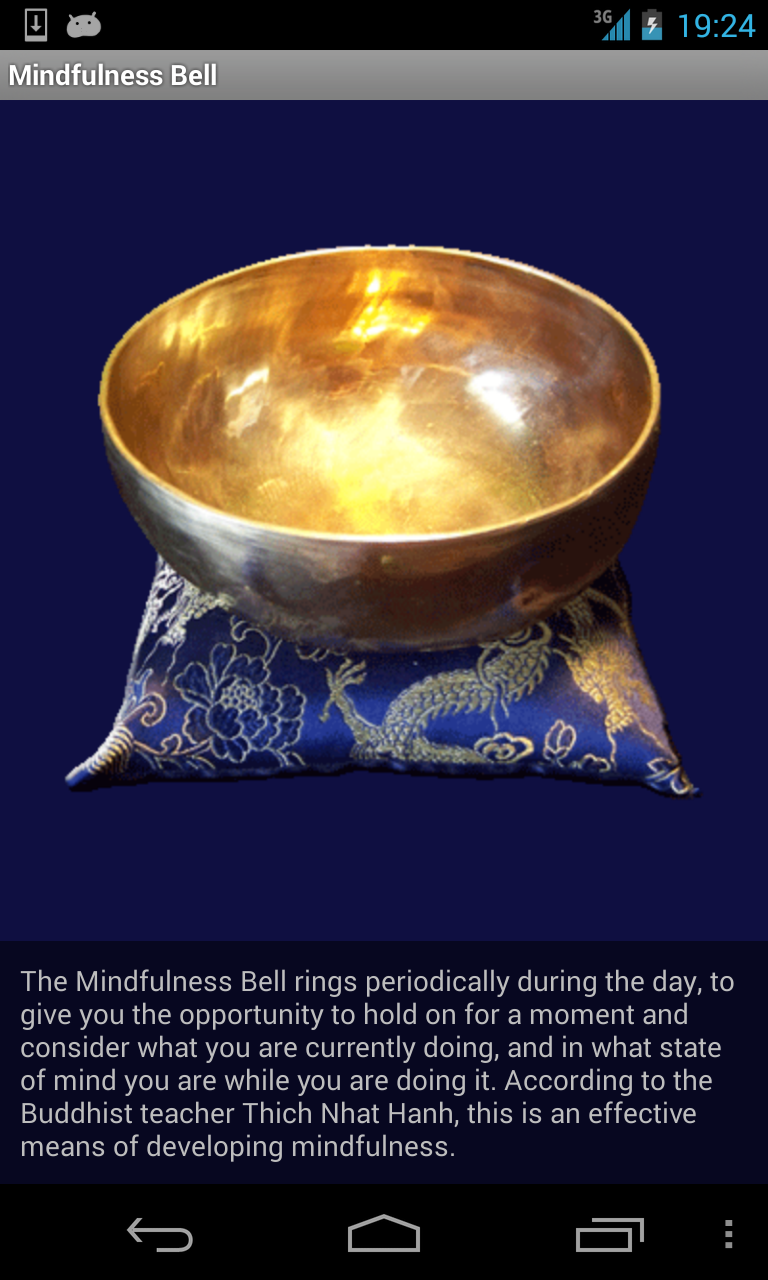
\includegraphics[width=0.24\textwidth]{figures/MB_main_screenshot.png}
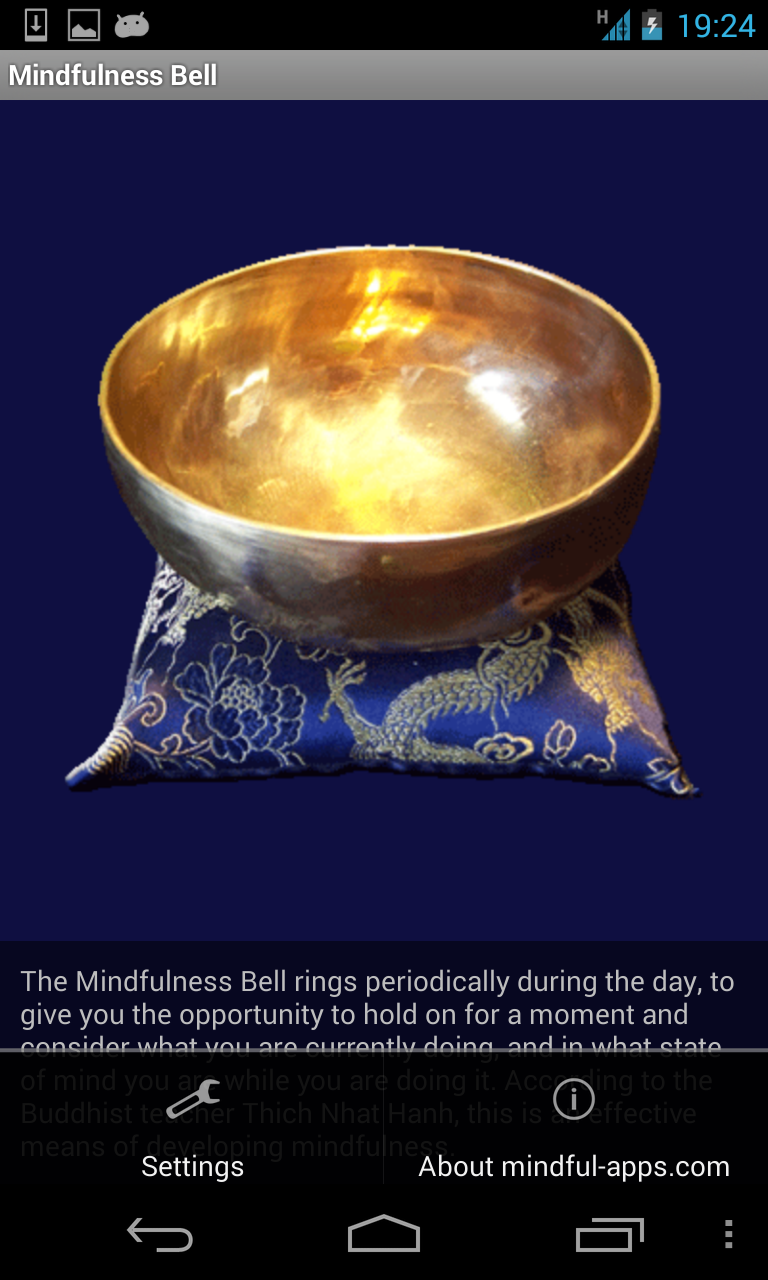
\includegraphics[width=0.24\textwidth]{figures/MB_menu_screenshot.png}
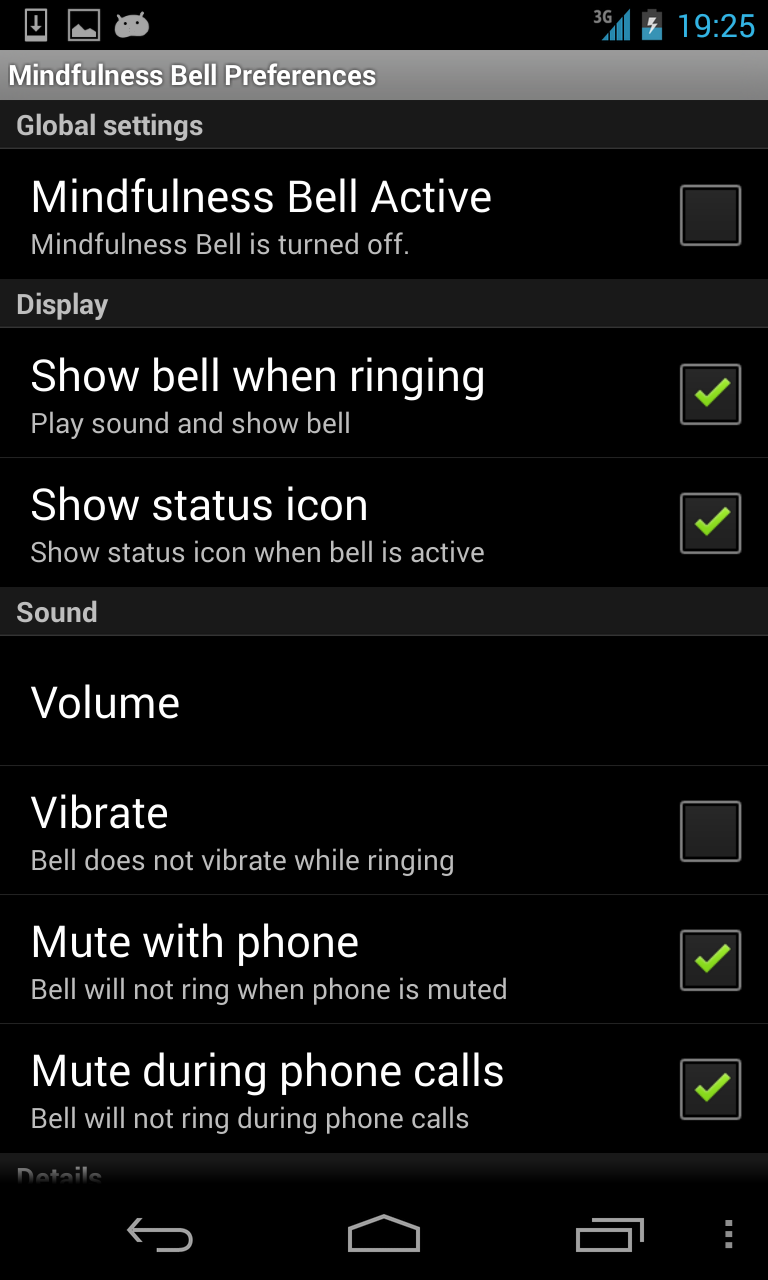
\includegraphics[width=0.24\textwidth]{figures/MB_preferences_screenshot.png}
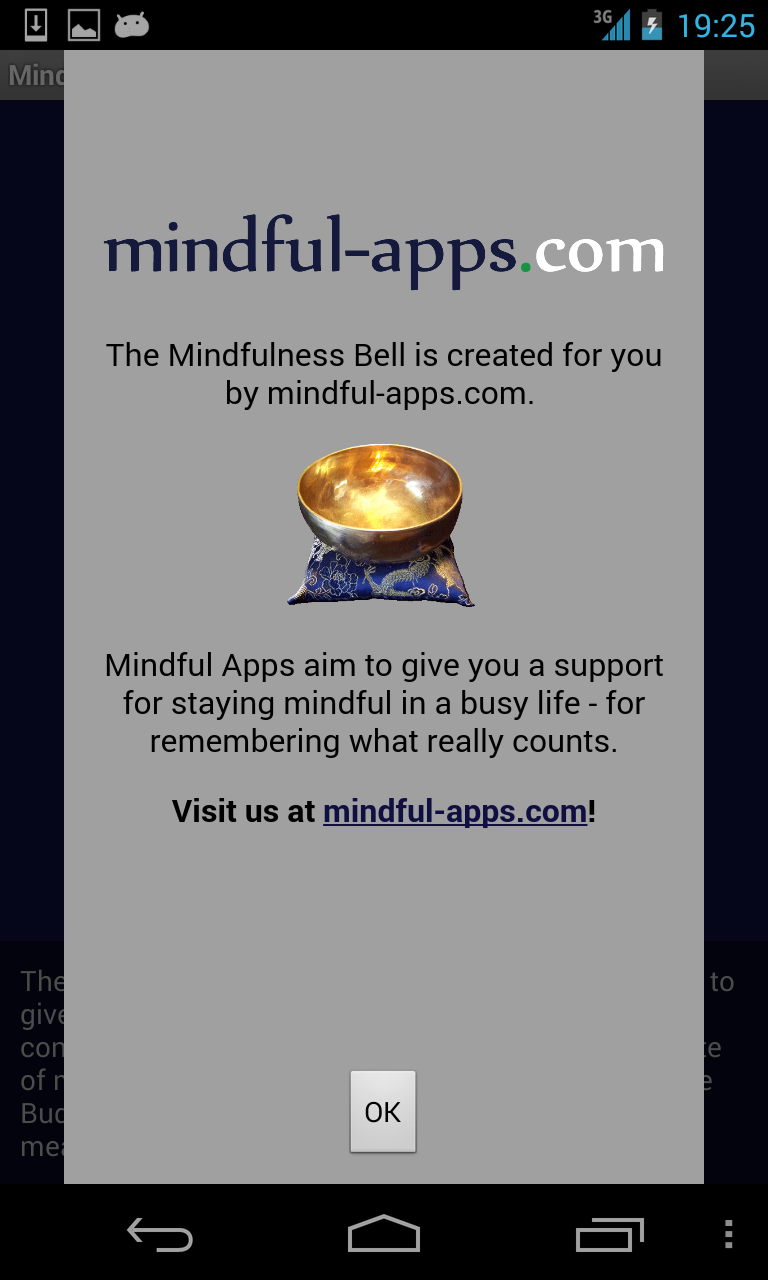
\includegraphics[width=0.24\textwidth]{figures/MB_about_screenshot.png}
\caption{Appearance of the screens of the Mindfulness Bell application.}
\label{fig:MB_allScreens}
\end{figure}

The preferences screen lets the user select the following options:

\begin{itemize}
\item Mindfulness Bell Active: Turn it on/off.
\item Show bell when ringing: shows the bell image on screen when it rings.
\item Show status icon: shows icon if bell is active.
\item Volume.
\item Vibrate: Device vibrates when the bell sounds.
\item Mute with phone: Bell does not ring if device is muted.
\item Mute during phone calls.
\item Ring bell about every...: User can choose 5, 10, 15, 30 minutes, 1, 2, 3 or 4 hours.
\item Start bell every day at... User can choose on the hour, from midnight to 11 PM.
\item Stop bell every day at... User can choose on the hour, from midnight to 11 PM.
\end{itemize}

Finally, the 'About' screen just shows the URL to the developers web page and a small text about them, again with the bell image. 

\subsubsection{Analysis of content}

The bell sound and image are the only real content of the application. The sound is easily noticeable but not too intrusive. 

\subsubsection{Analysis of business model and strategy}

The application is free, so business-wise it is just a way to advertise the development team. There is no extra content or in-app purchases available. 

\subsubsection{Critical Analysis}
The Mindfulness Bell is a simple idea turned into an application. It doesn't need a fancy interface, just a fast way to activate and configure it. The only visual setback is the position of the Menu button, located at the bottom right corner and very small in size. It would be better if the application made use of the Android's Action Bar with the menu button on the top right. 


\subsubsection{User's feedback}

On Google Play, the application has a 4.5 out of 5 rating with $1.820$ total opinions. The user's comments talk about how the app helps them to bring back attention to the present moment, which is one of the basic precepts of mindfulness. Reading the comments on xyo.net, they are also generally positive. A minority of users ask for more scheduling options and more accurate interval times.


\subsubsection{Wrap-up} 

This application shows that turning a really simple concept into an app can produce very good results if done properly. It is arguable how many people would pay for such a simple application, but the number of downloads it can get as a free application might be enough to make users check out other apps from the same developer.

%--------------------------------------------------------------
%			MEDITATE MEDITATION TRACKER
%--------------------------------------------------------------

\subsection{Meditate Meditation Timer}
\begin{wrapfigure}{l}{0.08\textwidth}
  \vspace*{-0.8cm}
  \begin{center}
    
\includegraphics[width=0.08\textwidth]{figures/MMT_icon.jpg}
  \end{center}
  \vspace*{-0.5cm}
\end{wrapfigure}
Meditate Meditation Timer is a simple, yet complete, meditation helper. Pre-recorded sessions (with no voice, just sound) guide the user's meditation and help him fall asleep or find affirmation. Both beginners and experienced meditators can use the app. The user can record his sessions and watch as he increases in duration and strength over time.\\
The app is only available for Android and it has both free version and a premium version which costs \euro{1.79}. The installations range between $1,000$ and $5,000$ and it has an average score of 4.4 out of 5. The App is designed by \textit{MeditateApp} which do not have other apps in Google's PlayStore. It was last updated the 3rd of September, 2013. 

\subsubsection{Features} 
The application has the following features:

\begin{itemize}
\item Choose between single mode or customizable meditation plans.
\item Make notes after each meditation's session. All of them will be stored in the history and statistic charts for further reviewing or editing.
\item Single mode is a customizable mode for quick setup of meditations in which it is possible to:
\begin{itemize}
\item Set up the duration of meditation (Hours:Minutes).
\item Select different Meditations: Normal Meditation, Meditation with Affirmation and Fall Asleep mode. Affirmation mode let's you to type and save the affirmation sentence you want to focus your meditation on. Fall Asleep category has always given setup for quieting the each next time sound is playing.
\end{itemize}
\item The meditation plans include programmable meditation plans with as many programmable steps as you want to have in. In this mode, it is possible to:
\begin{itemize}
\item Create as many plans as desired. 
\item Name and edit the plan title.
\item Create any amount of steps.
\item Choose the category of meditation for each step.
\item Set duration time for each step (Hours:Minutes).
\item Edit every previously created step.
\item Delete steps.
\item Edit current category step or its duration from the main window of application (directly after it has started).
\end{itemize}
\item The application features a statistics section which includes:
\begin{itemize}
\item Zoomable and scrollable statistics, divided into 7, 30, 90, 365 days and 'Show All' selectable options. Each select mode displays overall amount of hours/minutes of meditations for the chosen period of time.
\end{itemize}
\item There is also a History section in which information about the completed meditations can be checked. It is possible to:
\begin{itemize}
\item Check date, start and end time of meditation.
\item Category, note, affirmation, number of step, title of plan.
\item Edit previously created notes or create new ones.
\item Delete history entries.
\end{itemize}
\item Finally, the settings allow the user to:
\begin{itemize}
\item Choose between 9 beautiful meditation sounds.
\item Choose his own sound file from the phone storage.
\item Set the preparation time.
\item Set the sound repeating time.
\item Turn on/off the sound looping.
\item Turn on/off the functionality that fades out the sound. 
\item Automatic repetition of plan after completion.
\item Check how meditation sound files sound directly from the settings window.
\item Set time of daily notification.
\end{itemize}
\end{itemize}

\subsubsection{Analysis of the user interface}
The main screen is divided in three parts. The first part includes a bar located at the top in which the user can choose between the \textit{Single mode} and the \textit{Default Plan mode}. This bar spans $\sim 10\%$ of the screen. The second part spans $\sim 80\%$ of the screen and shows the meditation timer, the name of the meditation and a figure in the Lotus posture. By swiping the screen it is possible to choose between the three different types of offered meditations (\textit{Affirmation}, \textit{Medidation} and \textit{Fall Asleep}). The third part is a menu bar which is located at the botton and which has five sections: \textit{Stats}, \textit{History}, \textit{M (main screen)}, \textit{Plans} and \textit{Settings}.\\

Regarding the graphic design, the app is designed in brownish colors. Most of the buttons are beveled which makes the app look rather old (according to nowadays trends). \\ 

The navigation, usability and intuitiveness of the app are acceptable, however there are a couple of things which are quite anti-intuitive. First, to start the meditation, the user must push the big 'M' button located at the bottom. It may take a while to realize how to start the meditation. Additionally, there are no arrows nor any other symbols indicating that the main screen can be swiped to select between the different meditation types. Finally, when writing the message to be displayed in the Affirmation screen, the keyboard covers the message box so it is difficult to see what is being written. \\

We proceed now to analyze the four remaining sections of the app. 

\begin{itemize}
\item \textbf{Stats}: This section includes the duration of the completed meditations per day, week, month, 3 months, and year. The duration time is shown in big letters and by means of a bar plot to see the progression. The bar plot can be swiped both to the left and to the right to observe the desired time slot.
\item \textbf{History}: This section includes a history of all the carried out meditations. The user can check the starting and ending times, the duration, the type of meditation and the message that can be added at the end of the meditation. 
\item \textbf{Plans}: This section includes a meditation editor with which the user can create and edit meditation plans. A meditation plan is composed of as many steps as desired. Each of the steps can be configured to be one of the three available meditation types. Additionally, the time of each one of the steps can also be configured. The free version only allows a single (default) plan, while the premium version allows as many plans as desired. 
\item \textbf{Settings}: This section includes a series of options that can be configured by the user. Options include: preparation time, single mode duration, play sound every X seconds, loop sound, each next sound quieter, repeat plan after last step, plan steps auto continuation, change sound (a list of sounds is provided and the user can also select his own file), change ending bell, everyday notifications and set notifications time.
\end{itemize}

\begin{figure}[H]
	\centering
	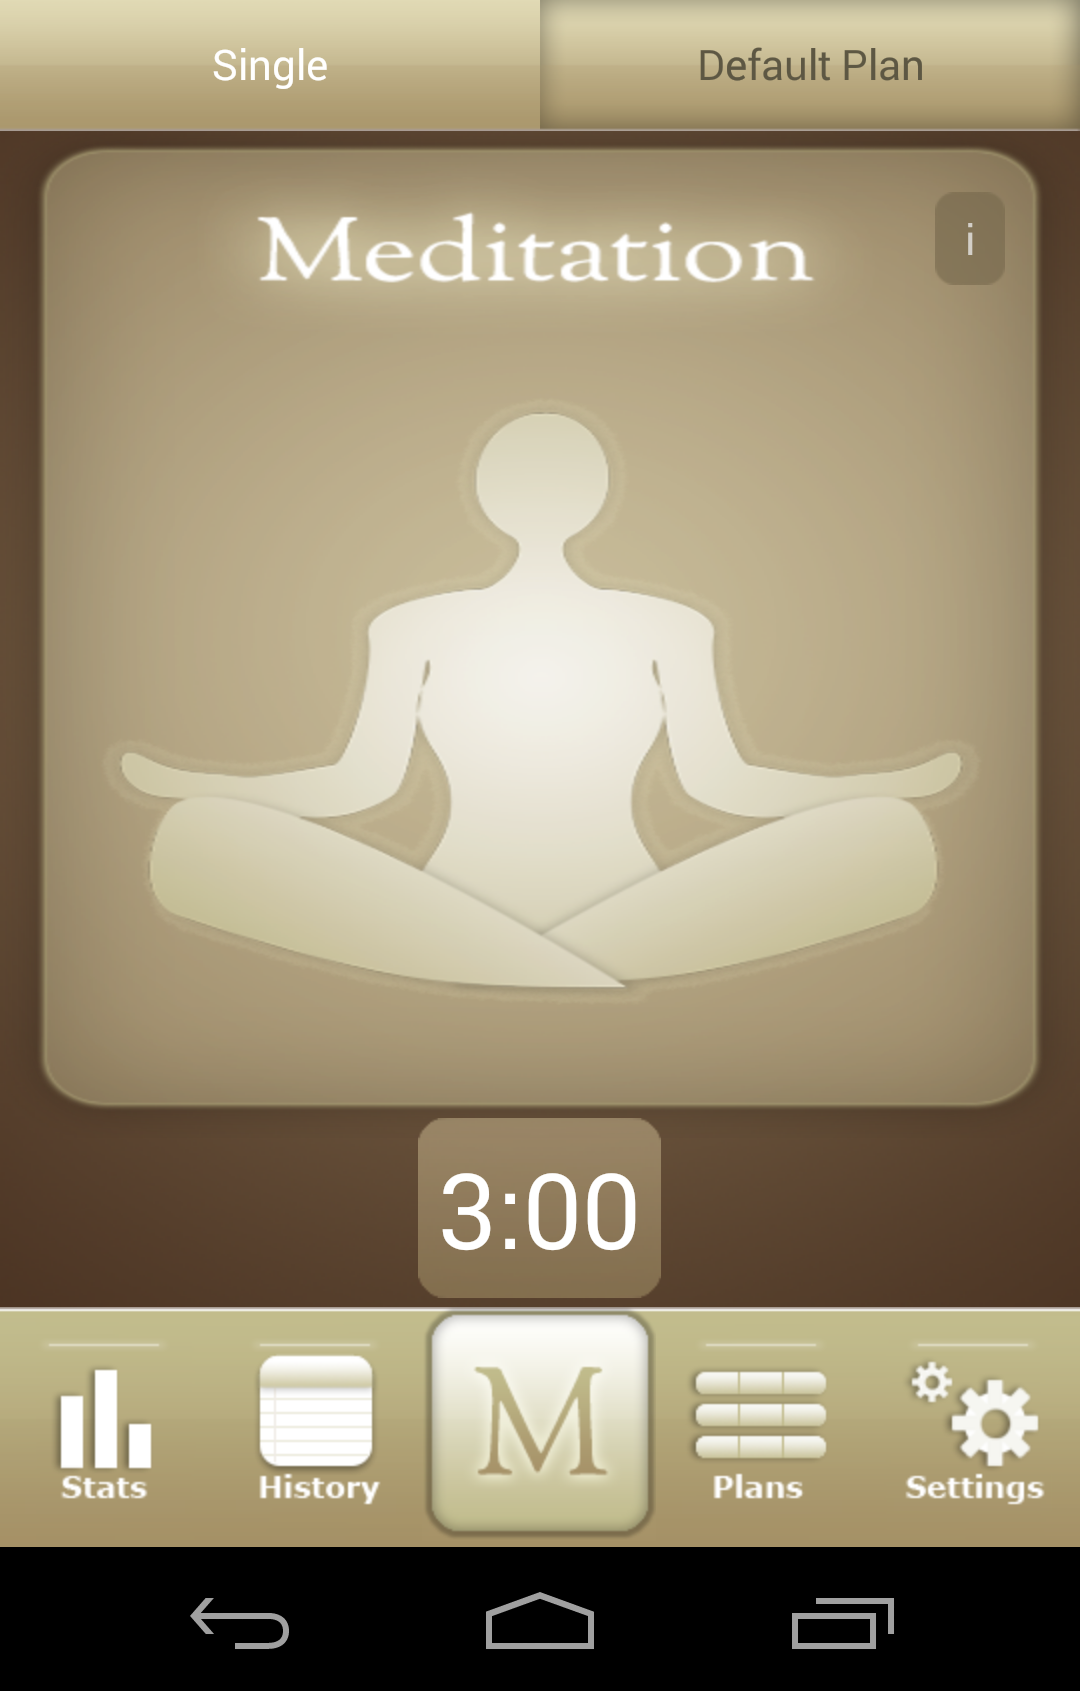
\includegraphics[width=0.20\textwidth]{figures/MMT_main_screen.png}
	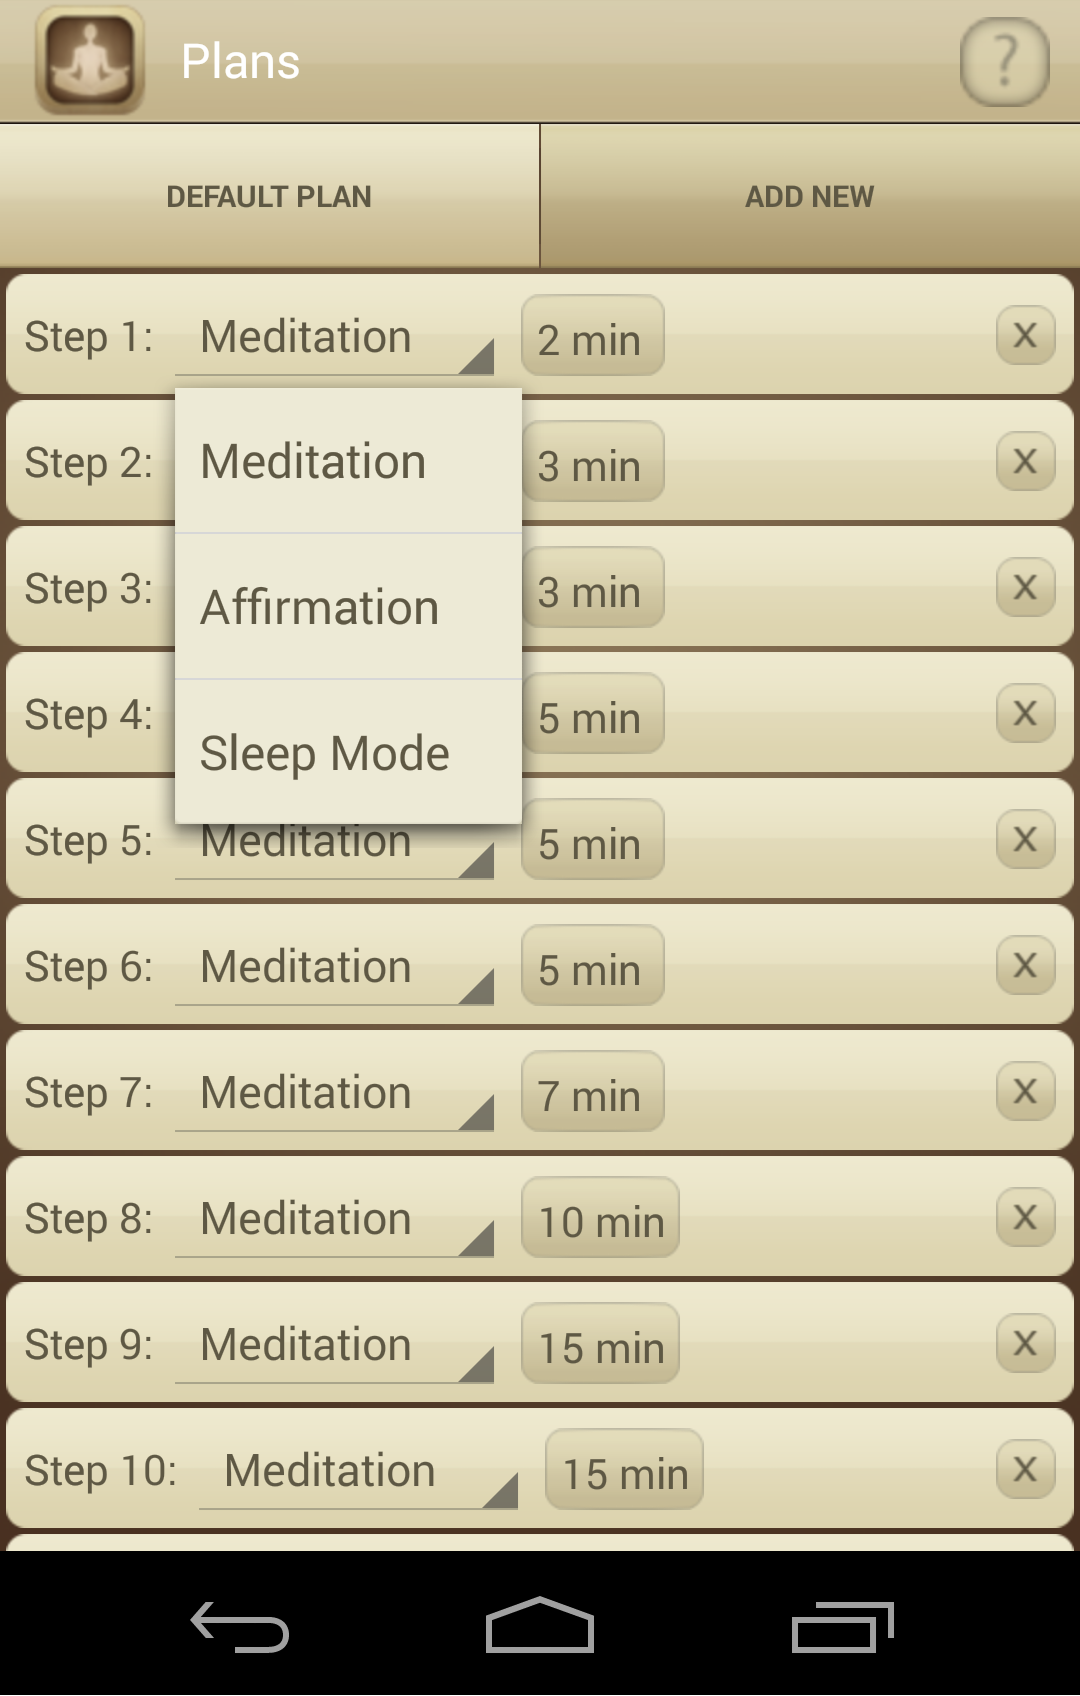
\includegraphics[width=0.20\textwidth]{figures/MMT_plan_screen.png}	
	\includegraphics[width=0.20\textwidth]{figures/MMT_stats_screen.png}
	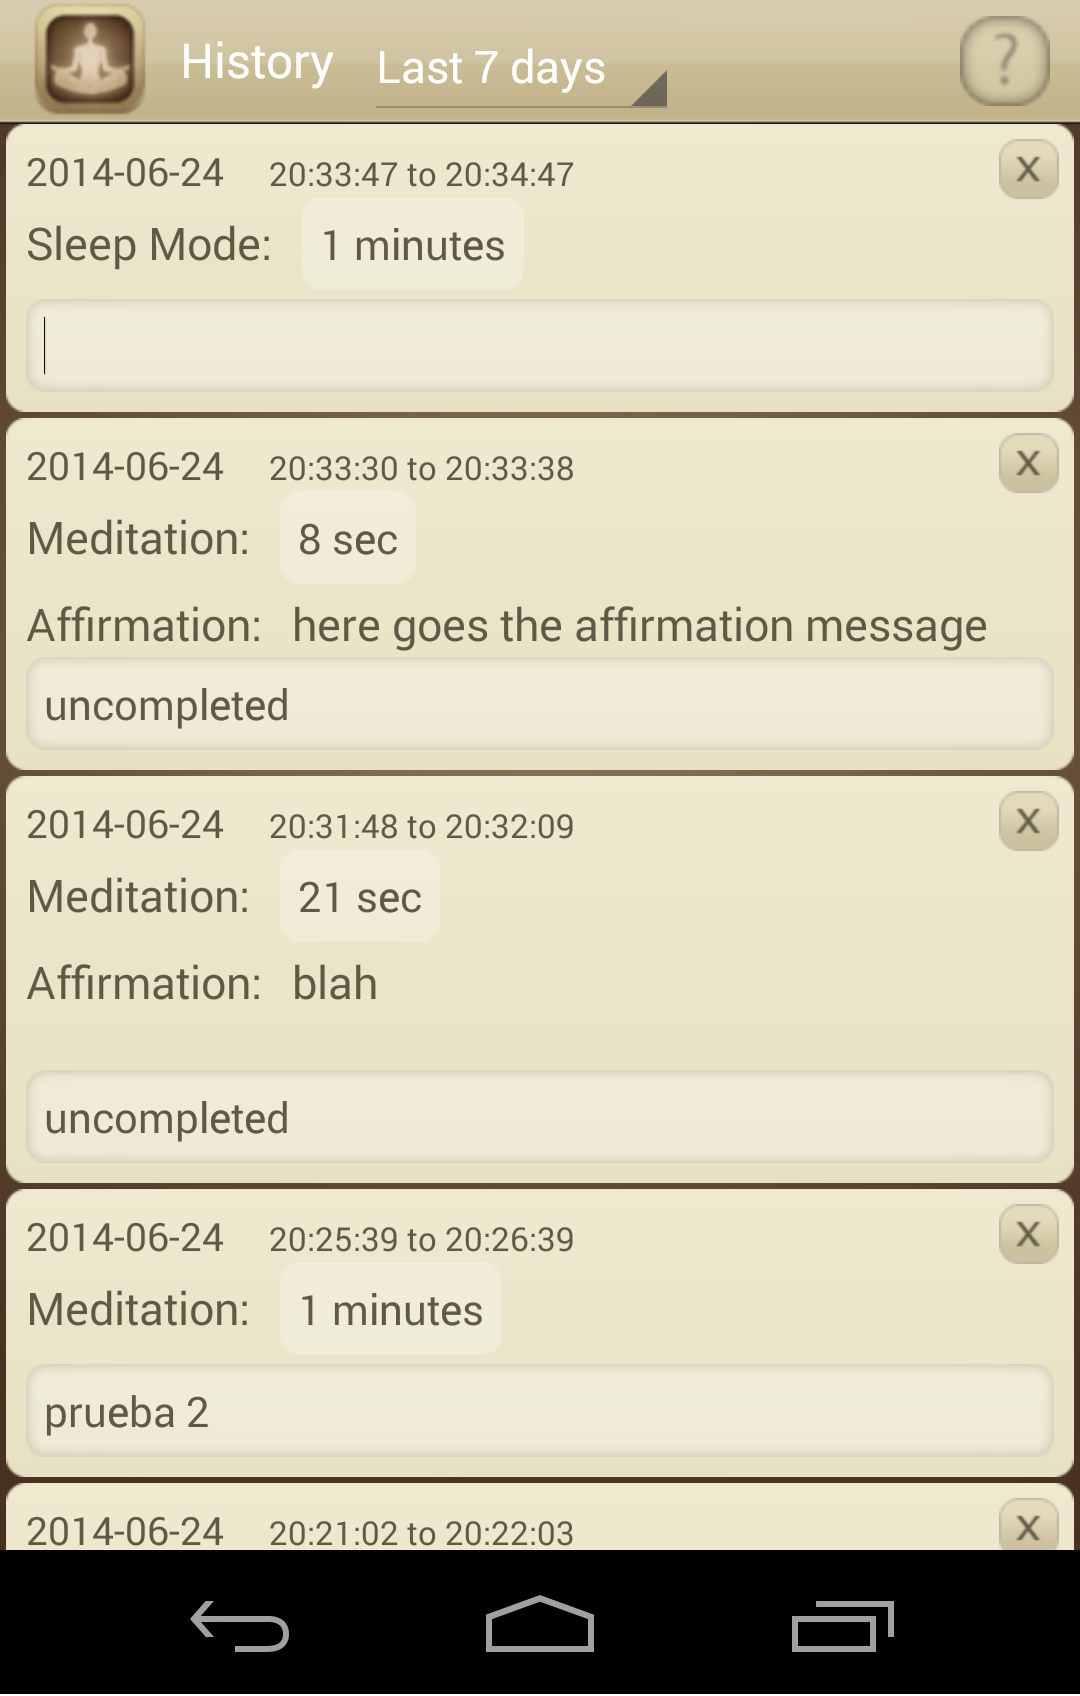
\includegraphics[width=0.20\textwidth]{figures/MMT_history_screen.png}		
	\label{fig:MT_meditation}
	\caption{Appearance of Meditation Timer screens}
\end{figure}

\begin{figure}[H]
	\centering
	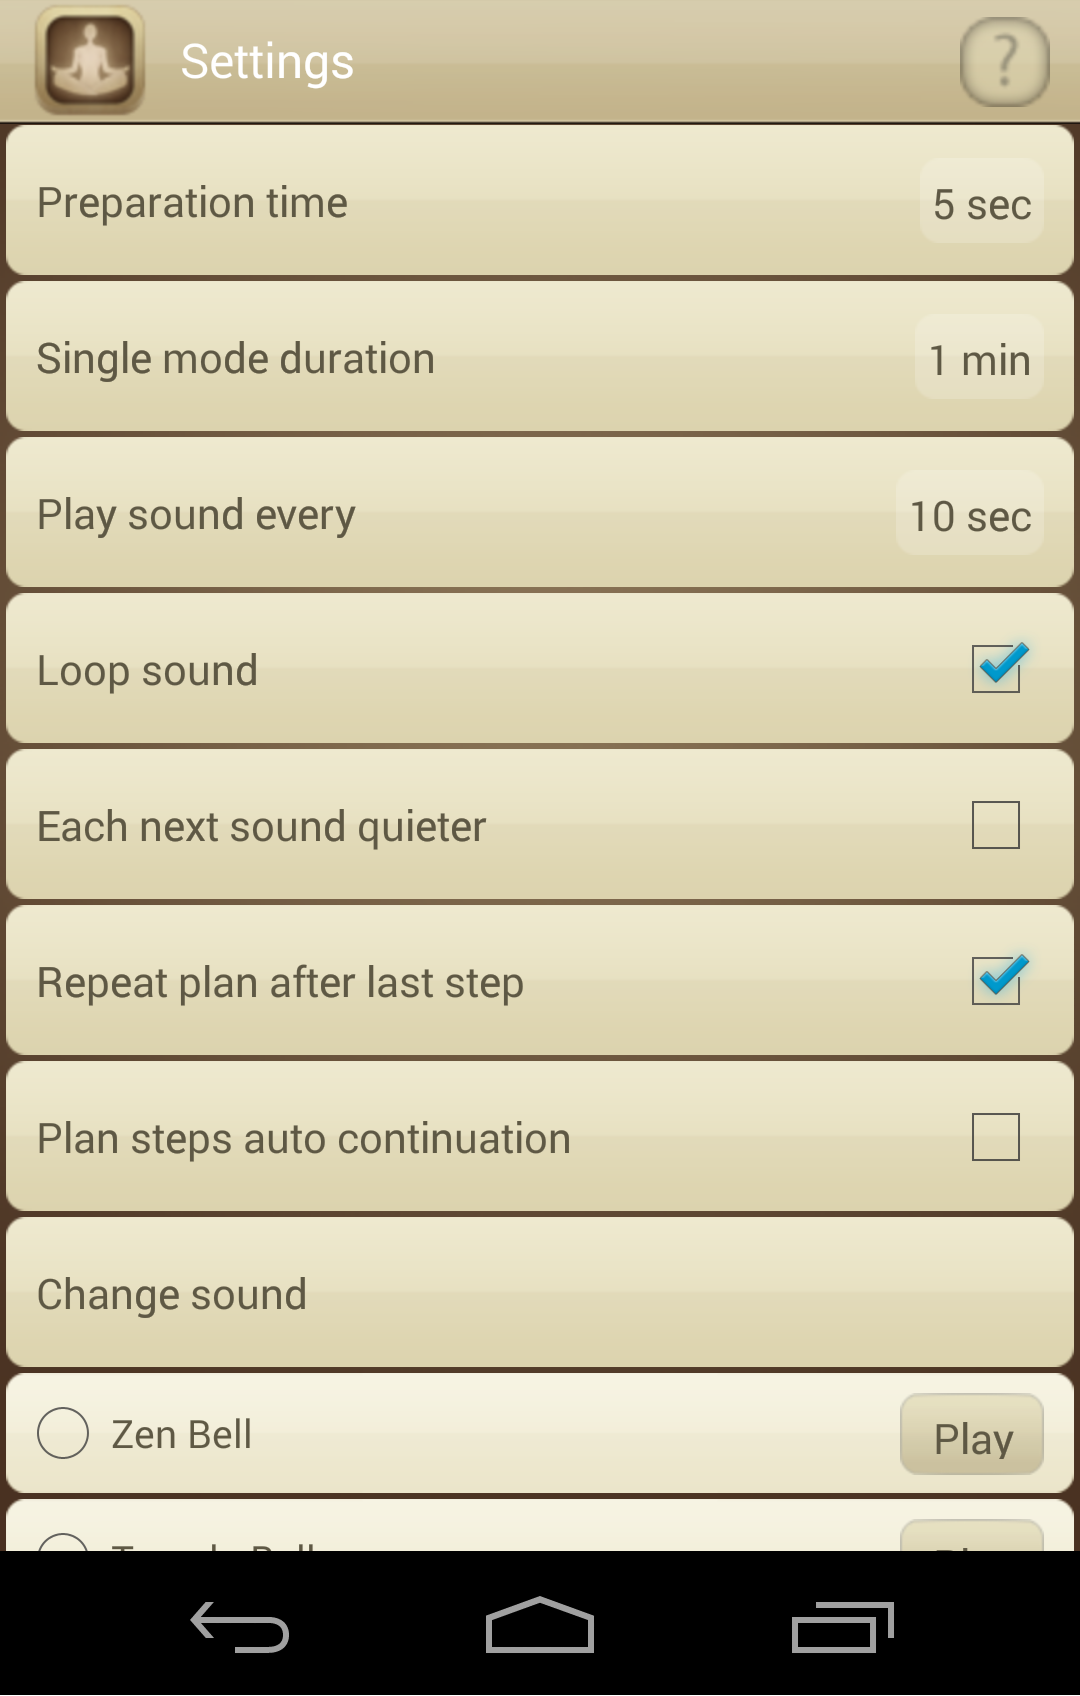
\includegraphics[width=0.20\textwidth]{figures/MMT_options_screen1.png}
	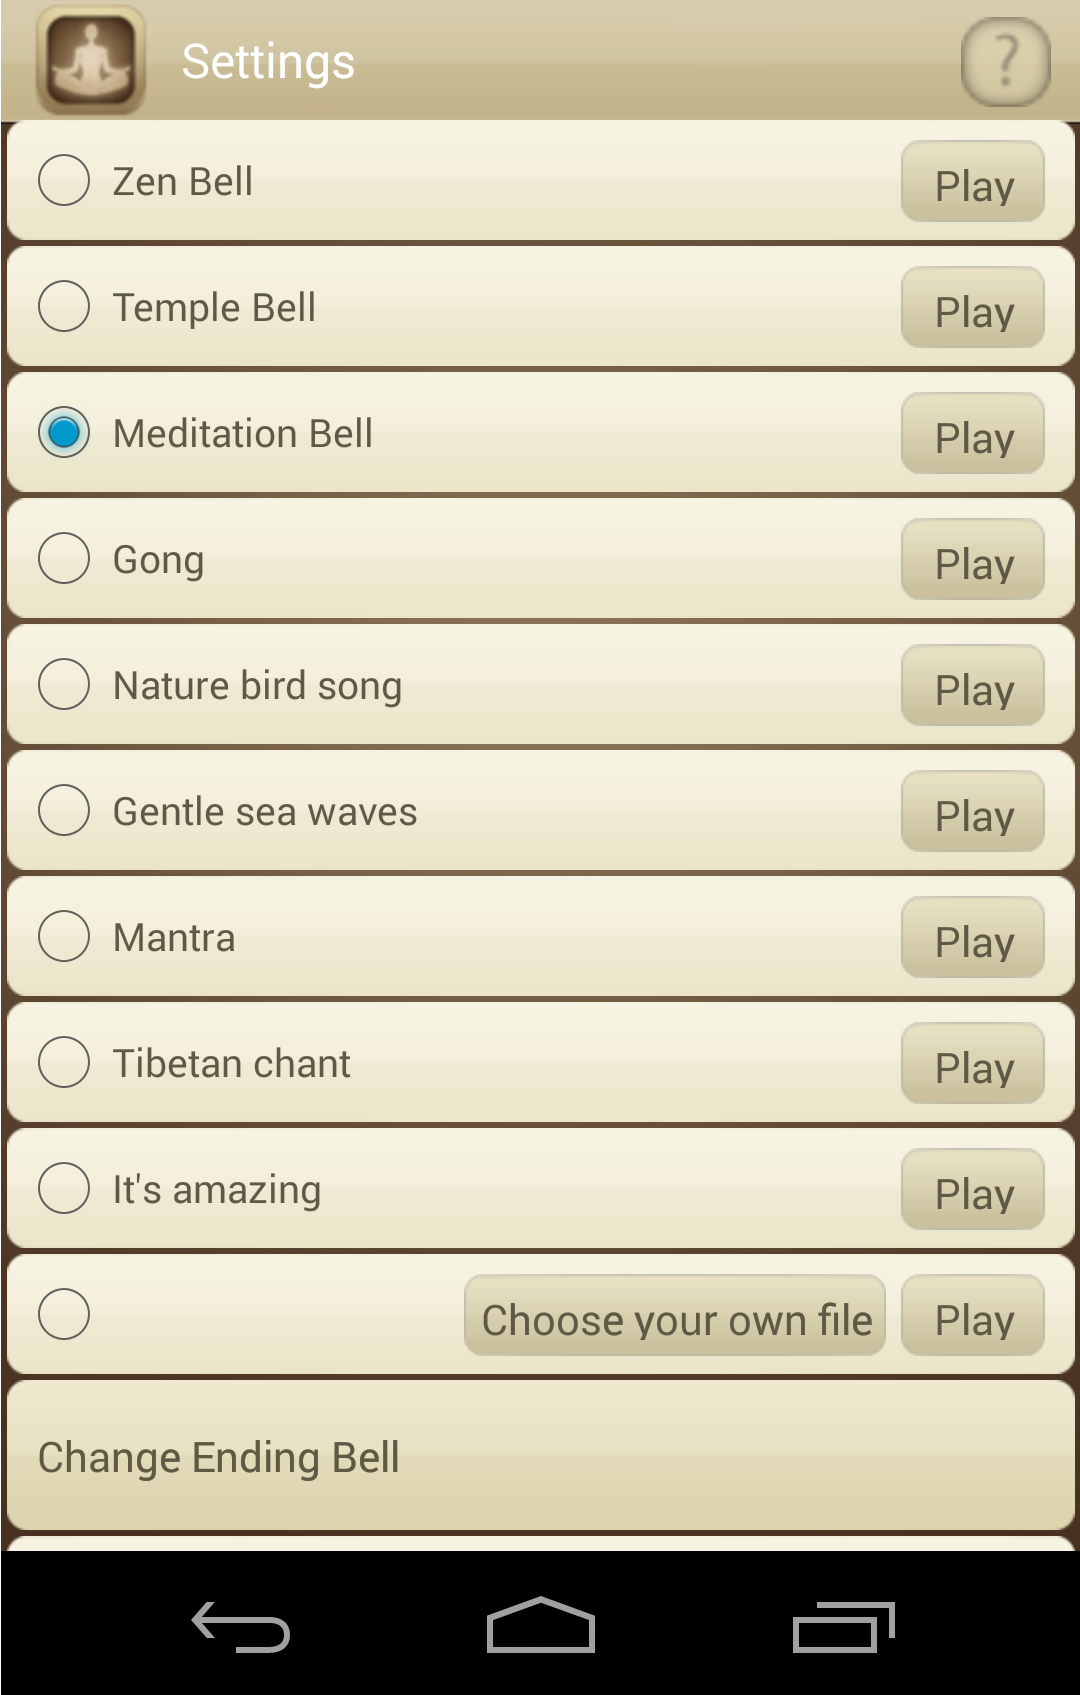
\includegraphics[width=0.20\textwidth]{figures/MMT_options_screen2.png}	
	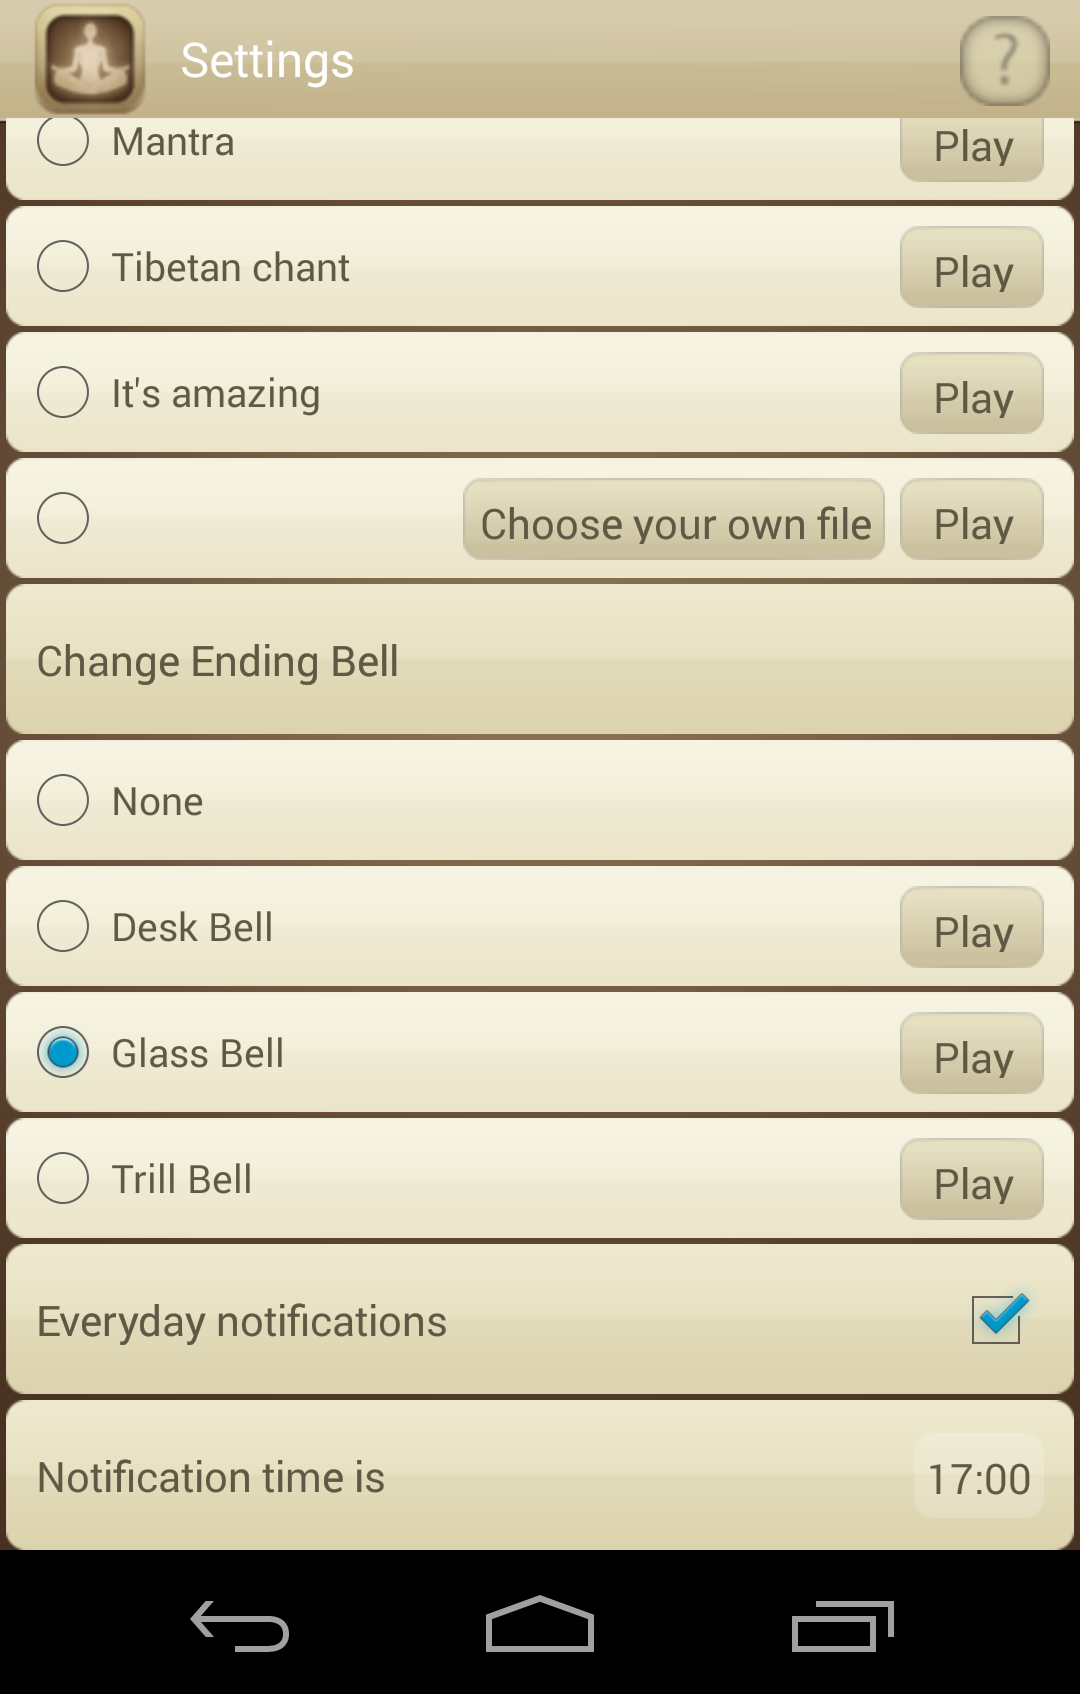
\includegraphics[width=0.20\textwidth]{figures/MMT_options_screen3.png}	
	\label{fig:MT_options}
	\caption{Appearance of Meditation Timer configuration screen}
\end{figure}

\subsubsection{Analysis of content}
TO BE COMPLETED

\subsubsection{Analysis of business model and strategy}
The application has a free version and a premium version. The free version includes ads at the top (spanning around $10\%$). Additionally, some of the functionalities are only available in the premium version. Some examples of the limited options are:
\begin{itemize}
	\item Statistics are only available for the last 7 days.
	\item Only one personalized meditation plan is allowed.
	\item The ending bell can not be changed.
	\item User own sound files can not be selected.
\end{itemize}

\subsubsection{Critical Analysis}
The application offers a simple yet complete meditation helper. However, the overall look and feel is improvable. It does not offer voice-guided meditations and its scope is very limited.  

\subsubsection{Users' feedback}
The users have a positive opinion of the application overall. Some of the things they criticize are listed below.
\begin{itemize}
	\item Low quality of the sounds.
	\item Low volume of the sound indicating the end of the meditation.
	\item Inability to manually modify the history of meditations.
	\item Having to click a button to start the next meditation step.
	\item Notifications from other applications are not silenced.
\end{itemize}
Consequently, the users suggest the following,
\begin{itemize}
	\item Add the average time meditated per day.
	\item Ability to add/delete entries in the log manually. 
	\item Ability to export the log.
	\item Ability to backup all the logs and history to, for example, Google Drive.
	\item Increase the amount of Tibetan bowl sounds available.
	\item Add auto-sharing when a meditation is finished (social networks).
	\item Ability to add each one of the meditations (in time, type, etc.).
	\item Silence notifications from other applications during the meditation.
\end{itemize}
They like the application for the following reasons,
\begin{itemize}
	\item It is very good to get initiated in meditation as it offers short meditations.
	\item It is very good to maintain regular meditations.
	\item It is simple, flexible and honest.
	\item The choice of sounds is very wide.
	\item The affirmations are very useful.
\end{itemize}

\subsubsection{Wrap-up}
The Meditation Timer app offers a set of configurable simple meditations. It allows the user to select the duration and the sound which is being played in the background. The interface has a poor look and feel mainly due to the selected color scheme. The business model is based on a pay-per-download approach with both a free version with limited functionality and a full premium version. The application has in general a positive feedback by the users. The application is only available in english.

% -----------------------------------
%        MINDFULNESS FOCUS NOW
% -----------------------------------

\subsection{Mindfulness Focus Now}
\begin{wrapfigure}{l}{0.08\textwidth}
  \vspace*{-0.8cm}
  \begin{center}
    
\includegraphics[width=0.08\textwidth]{figures/MFN_icon.png}
  \end{center}
  \vspace*{-0.5cm}
\end{wrapfigure}
Mindfulness Focus Now (MFN), is a meditation helper focused on keeping the user from distraction and being aware of the thoughts that do distract him. It is offered by Marcial Arredondo Rosas, part of the "Mindfulness\&Psicolog�a Barcelona" team. Marcial is a Clinical Psychologist currently researching for the UAB about mindfulness training. The application is being used as a tool in his research. \\

The application is offered for free, both for Android and iOS. It has been downloaded around $5.400$ times from the Play Store and around $4.000$ from the Apple AppStore (estimated by xyo.net). The Android version was last updated Oct 10 2013, and the iOS version on Oct 17 2013.\\

The application is not localized, being offered only in the Spanish language.

\subsubsection{Features} 

The developer doesn't offer a list of features, here we show the list made after careful analysis of the application:
\begin{itemize}
\item Five different guided meditations.
\item Distraction log: while meditating, record each distraction with duration (less than 10 sec, 10 sec to 1 min, more than 1 min) and kind of thought (neutral, positive, negative or mixed).
\item Send by email the distraction log (as plain text).
\item Time Box Mindful: Use the distraction log for any activity that requires concentration for a certain amount of time.
\item Three tutorial videos.
\end{itemize}

The only distinguishing feature of this app from others is the distraction log, but the raw results it presents may be hard for the average user to interpret. \\

\subsubsection{Analysis of the user interface}

We will analyse the Android application, which is the one we have access to. The main interface is a simple list in orange and white, which gives access to every feature of the app. There is a fixed button on the bottom to give faster access to the silent practice.\\

In the figure \ref{fig:MFN_allScreens} the splash screen and the main menu are shown. 

\begin{figure}[H]
\centering
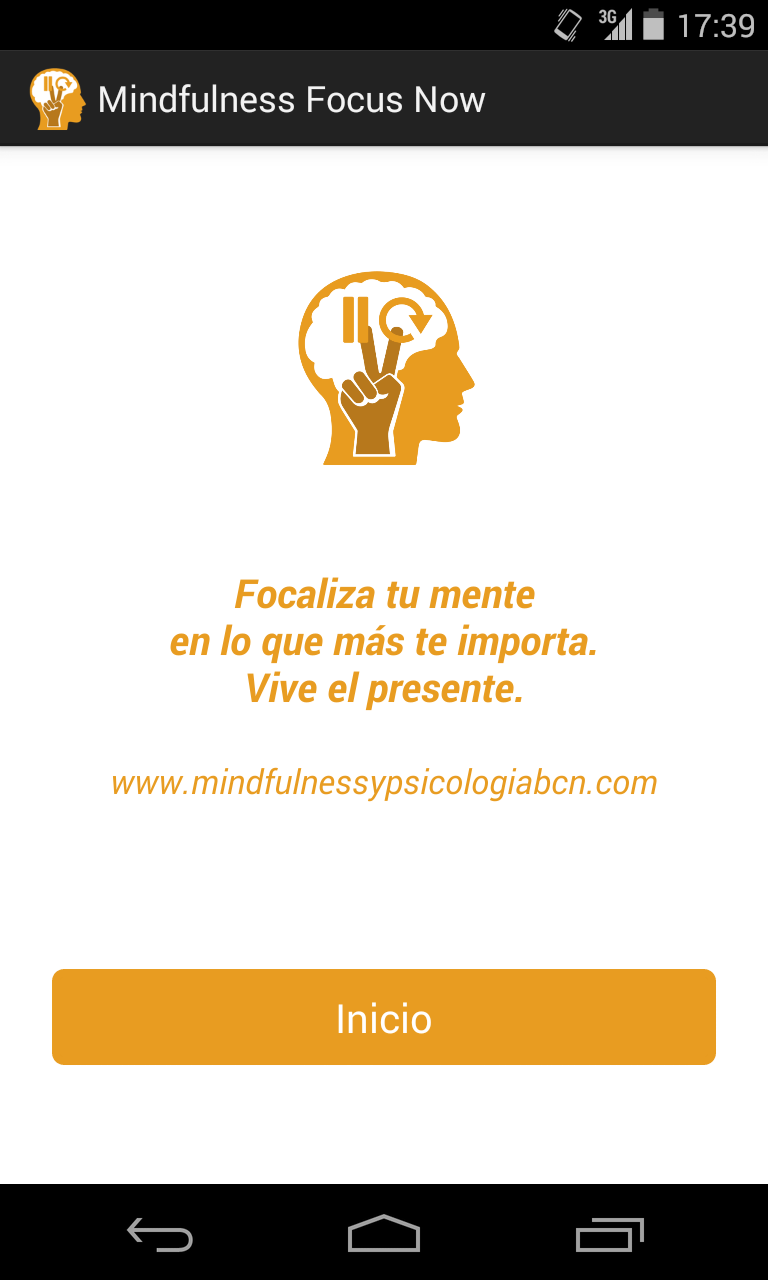
\includegraphics[width=0.32\textwidth]{figures/MFN_splash_screenshot.png}
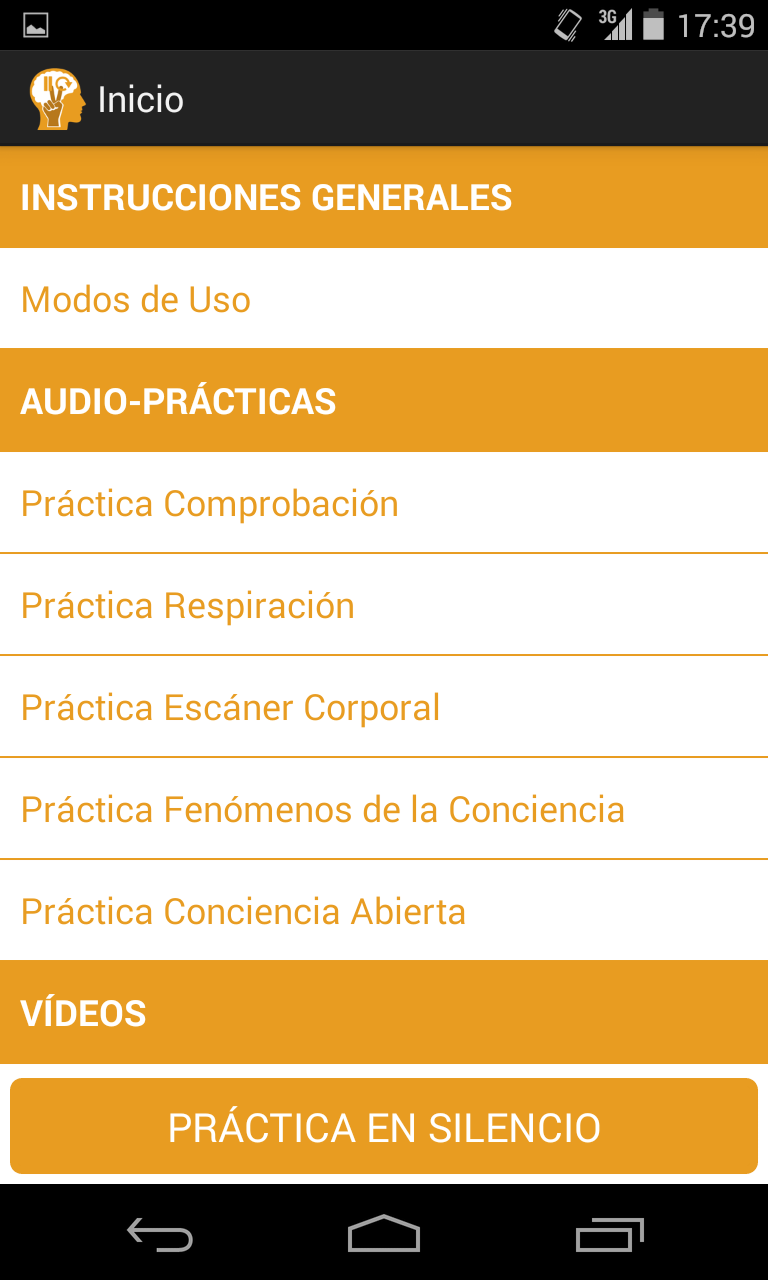
\includegraphics[width=0.32\textwidth]{figures/MFN_menu1_screenshot.png}
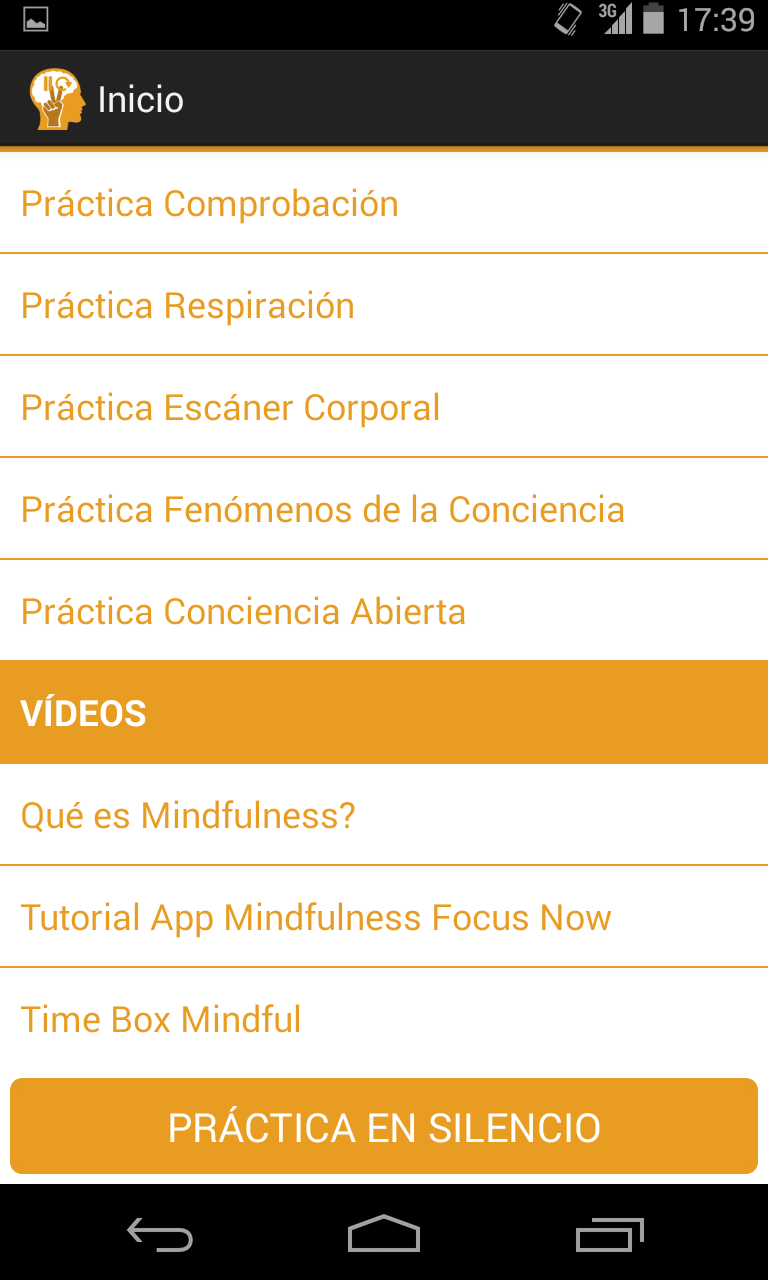
\includegraphics[width=0.32\textwidth]{figures/MFN_menu2_screenshot.png}
\caption{Appearance of the splash screen and menu of the Mindfulness Focus Now application.}
\label{fig:MFN_allScreens}
\end{figure}

The use instructions are just a text screen with an explanation on how to use the distraction log screen that we will show later. The video list shown in the menu directly takes the user to the Youtube application or the browser to watch the video. The Silent Practice option lets the user select the duration before starting. \\

In figure \ref{fig:MFN_moreScreens} we can see the duration selection for the Silent Practice, the practice interface and the distraction log results.

\begin{figure}[H]
\centering
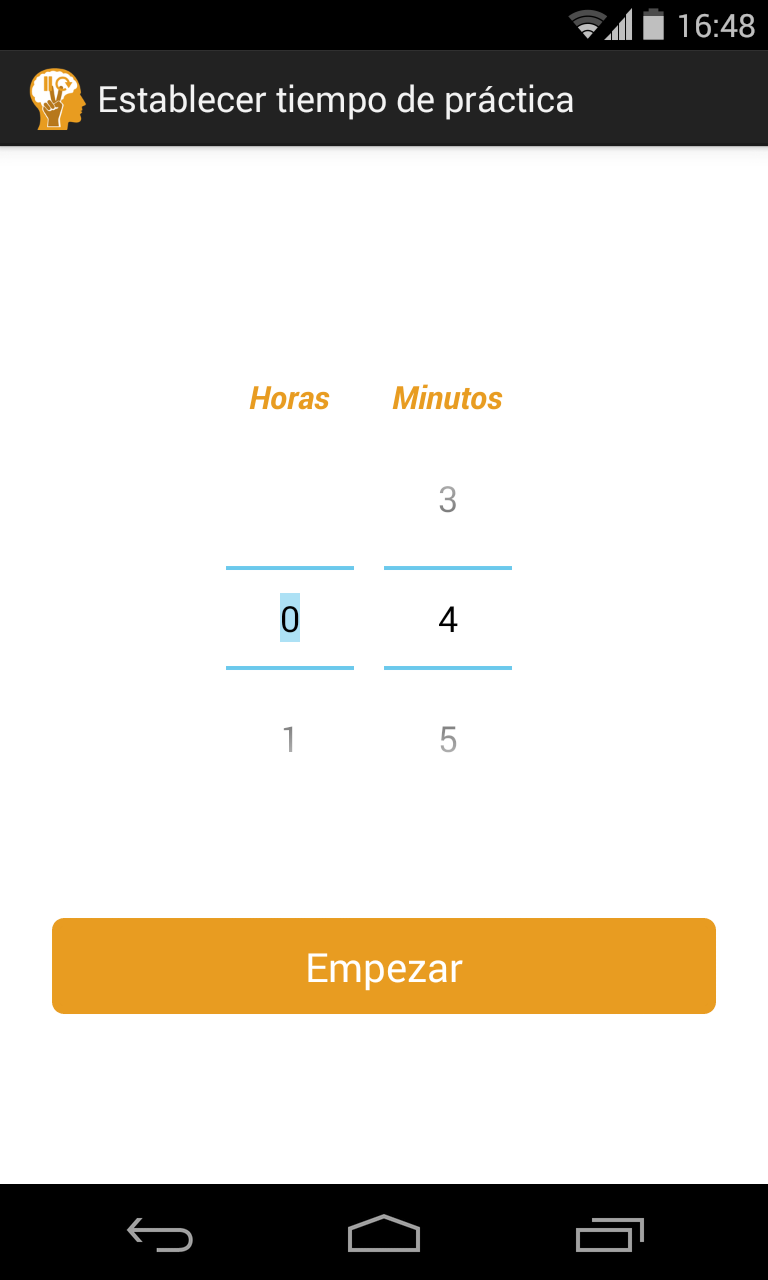
\includegraphics[width=0.32\textwidth]{figures/MFN_duration_screenshot.png}
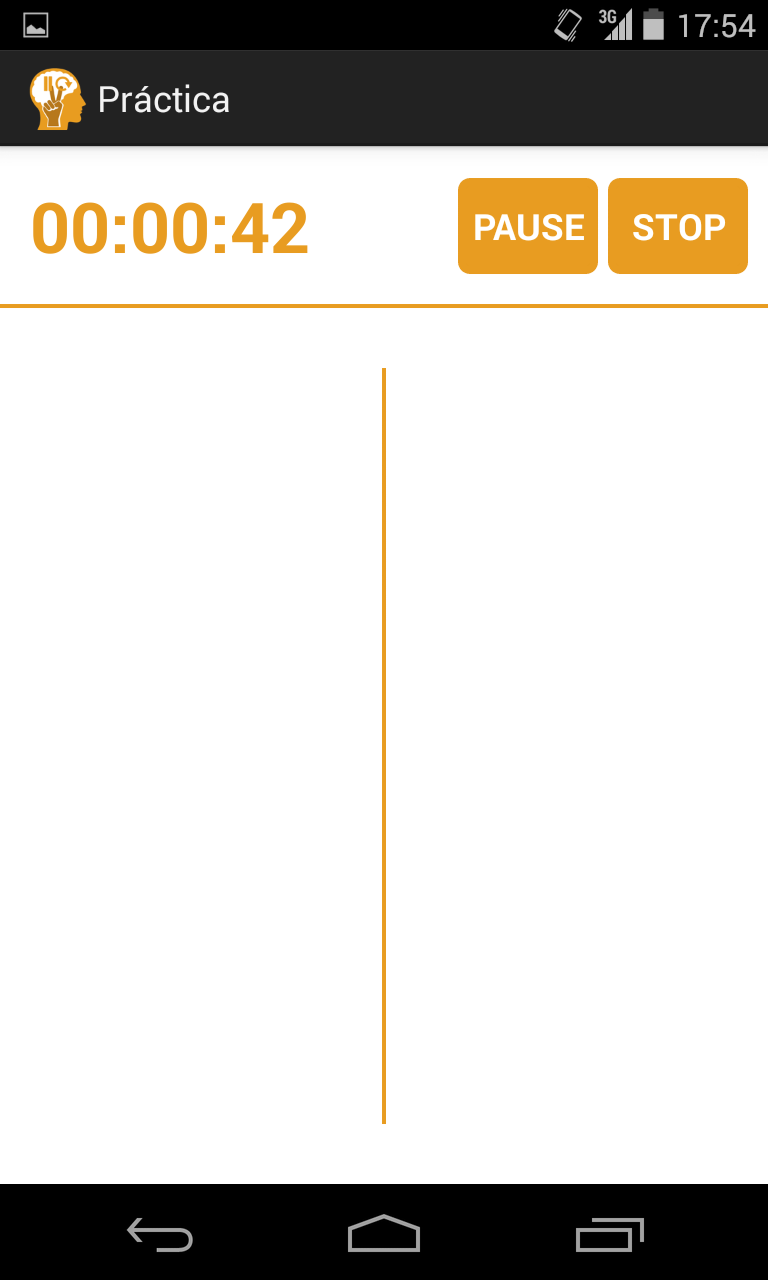
\includegraphics[width=0.32\textwidth]{figures/MFN_meditation_screenshot.png}
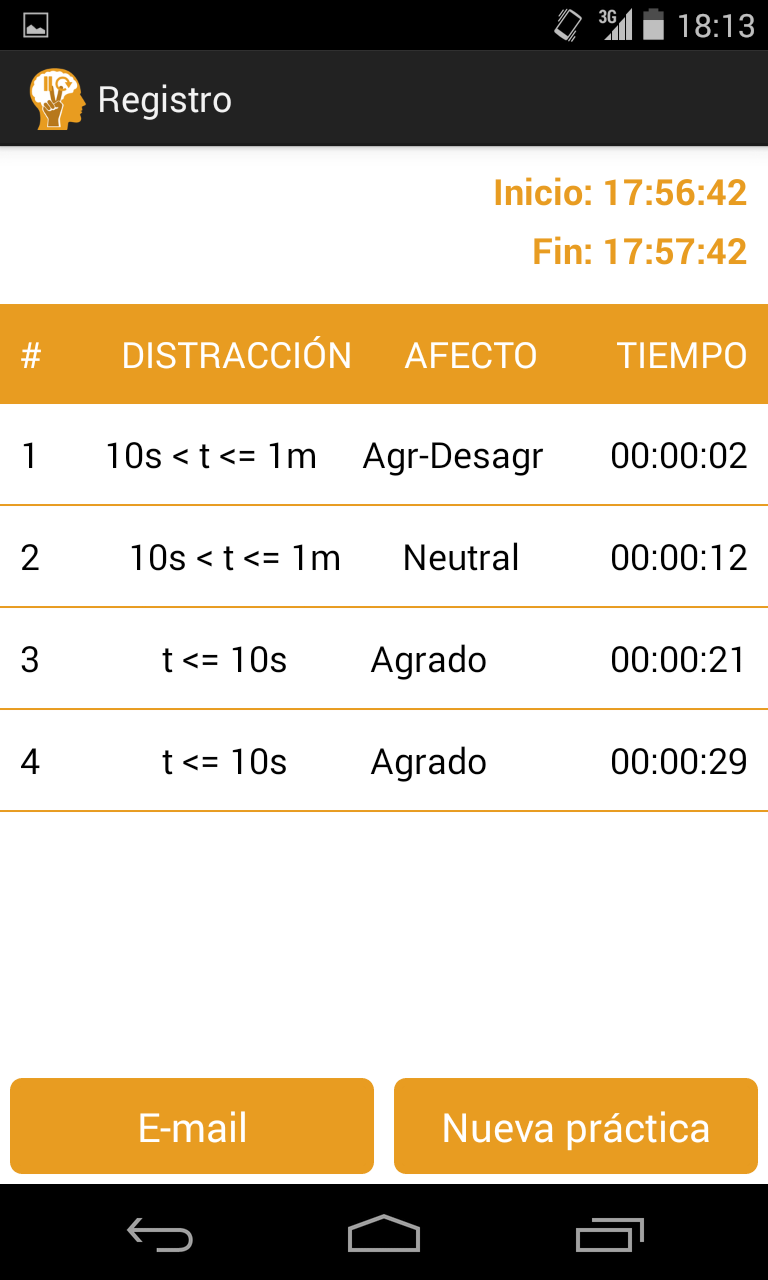
\includegraphics[width=0.32\textwidth]{figures/MFN_distraction_log_screenshot.png}
\caption{Appearance of the duration selection, practice and results for the Mindfulness Focus Now application.}
\label{fig:MFN_moreScreens}
\end{figure}

The duration selection uses the native time spinner, the design is clean and consistent with the rest of the application. The meditation screen shows a countdown timer, Play/Pause and Stop buttons on top. The rest of the screen is split in half vertically, and is used to record the distractions. The number of taps on each side lets the user input the duration and kind of distraction. Finally, after the practice ends the distraction log is shown; it is a simple list containing every distraction logged with duration, kind and time into the practice when it happened. On the bottom of the screen there are to buttons, one lets the user send the log by email, the other goes back to the main menu after alerting the user that the results will be erased on exit.

\subsubsection{Analysis of content}
TO DO:TRY TO LISTEN TO THE MEDITATIONS

\subsubsection{Analysis of business model and strategy}

The application is free of charge, and there are no other revenue sources like in-app purchases or advertising. Our guess is this application has been developed in the context of Marcial Arredondo's PhD research, as a tool to collect meaningful data. 

\subsubsection{Critical Analysis}
As it has been said earlier, the application looks more like a tool for a specific research than a end-user driven approach. Still, some of its features could be of interest to the user looking for free meditation applications, specially in the Spanish language, since it is one of the few applications analysed with content in Spanish. \\

The distraction log system may be too complex for the average user, since it requires him to memorize the number of taps that represent each duration and kind of distraction, and then use it in a moment that he's supposed to not be thinking about anything. \\

The user interface is simple, but well thought out and coherent across the whole application. \\

The content.... LISTEN TO THE MEDITATIONS

\subsubsection{Users' feedback}

On Google Play, the application has a 4.0 out of 5 rating with 47 total opinions. The comments are generally positive, but the users say they are doing the practices without using the screen (the distraction log feature), since they have to think which side of the screen to tap and how many times, which further aggravates the loss of concentration.  \\

On iTunes App Store, the application doesn't have enough ratings. There are only two comments, that praise the application's content and professional look.\\

\subsubsection{Wrap-up}

Even though the application is primary developed as a tool for a specific research, it has reached almost $10.000$ downloads between iOS and Android, and more important it has been given positive feedback from the users. Since there are so few applications with content in Spanish, users are willing to try them even if the look is not very fancy. \\


% -----------------------------------
%        OMVANA
% -----------------------------------

\subsection{Omvana}
\begin{wrapfigure}{l}{0.08\textwidth}
  \vspace*{-0.8cm}
  \begin{center}
    
\includegraphics[width=0.08\textwidth]{figures/OMV_icon.png}
  \end{center}
  \vspace*{-0.5cm}
\end{wrapfigure}
Omvana is a meditation and content provider application, developed by Mindvalley Creations Inc. Mindvalley is a digital publishing company based in Kuala Lumpur (Malaysia), specialised in the areas of personal growth, entrepreneurship, lifestyle applications, and continuous education. Mindvalley employs 100+ people, it was featured in Inc. Magazine's Top 10 World's Coolest Offices and won WorldBlu's global Most Democratic Workplace Award for 7 years in a row. \\

The application works as a content market, providing a mix of free and paid sound tracks (music and spoken). It then lets you listen to the tracks and even mix any spoken track with any music track on the background.\\

Omvana is offered for free, both for Android and iOS. It has been downloaded around $1.000$ times from the Play Store and around $502.000$ times from the Apple AppStore (estimated by xyo.net). The cause for this huge difference in downloads is that the Android version was very recently added to the store. The full name of the iOS version is ``Omvana - Meditate, Sleep, Focus, Relax, Rest \& Nap Better with 1000s of Mindfulness, Hypnosis, Meditation and Binaural Sounds'', probably used as a SEO trick to get more results for every keyword used in the name. \\

The application is not localised, being offered only in the English language.


\subsubsection{Features} 

The features described by the developer are:

\begin{itemize}
\item 1000s of high-quality audio tracks, ambient sounds, binaural beats and narrated guides.
\item Your own Omvana mixing board ? mix and match any two of your favorite tracks.
\item Listen to narrated lessons and guides by inspiring thought leaders, like Bob Proctor and Martin Luther King, Jr
\item Sleep better with access to a powerful library of Sleep enhancement sounds
\item Deepen your experience with a library of calming ambient tunes and background sounds, featuring cutting-edge binaural beats technology
\item Transform and grow with access to powerful guided visualizations for every aspect of your personal growth from many best-selling authors.
\item Mix and match custom tracks to help you effortlessly achieve your goals ? stress relief, better health, heightened focus, even wealth and abundance
\item Record your own meditations and customize them using our mixing tool.
\item Get more out of your guided meditations with interactive track notes and video tips.
\item Expand your personal library whenever you want ? record your own guided meditations, or easily preview and purchase new tracks from the Omvana store 
\end{itemize}

In our own analysis of the application, we didn't find the option to record your own meditations. It may be well hidden in an obscure menu or maybe it was added to the feature list before it has been implemented. \\

\subsubsection{Analysis of the user interface}

We will analyse the Android application, which is the one we have access to. The home screen is a grid view with thumbnails of the available tracks for the user to listen. Android's Action Bar is conveniently customized at the top, with the Store icon on the left and the Mixer icon on the right.\\

The mixer shows two rows of round thumbnails, the top one containing the ambient sounds/music and the bottom one the vocals. The thumbnails can be swiped left or right to select the desired ambient and vocal tracks. A slider lets the user calibrate the balance between the ambient and the vocals. Finally, at the bottom, a Play/Pause button and a Heart to make the combination of ambient and vocals a favourite. If the user later selects one of the tracks and enters the mixer, it will select by default the favourite combination. \\

In the figure \ref{fig:OMV_HomeMixerScreens} the home screen and the mixer are shown.

\begin{figure}[H]
\centering
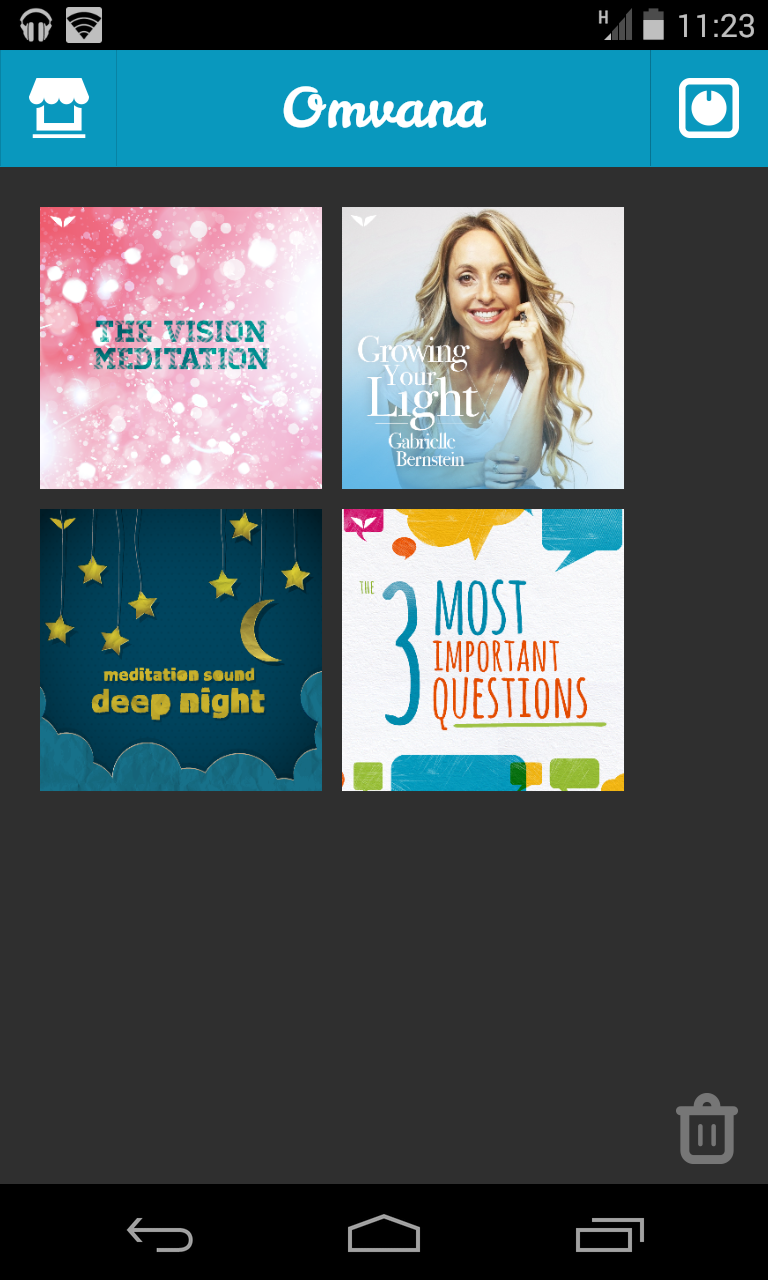
\includegraphics[width=0.45\textwidth]{figures/OMV_home_screenshot.png}
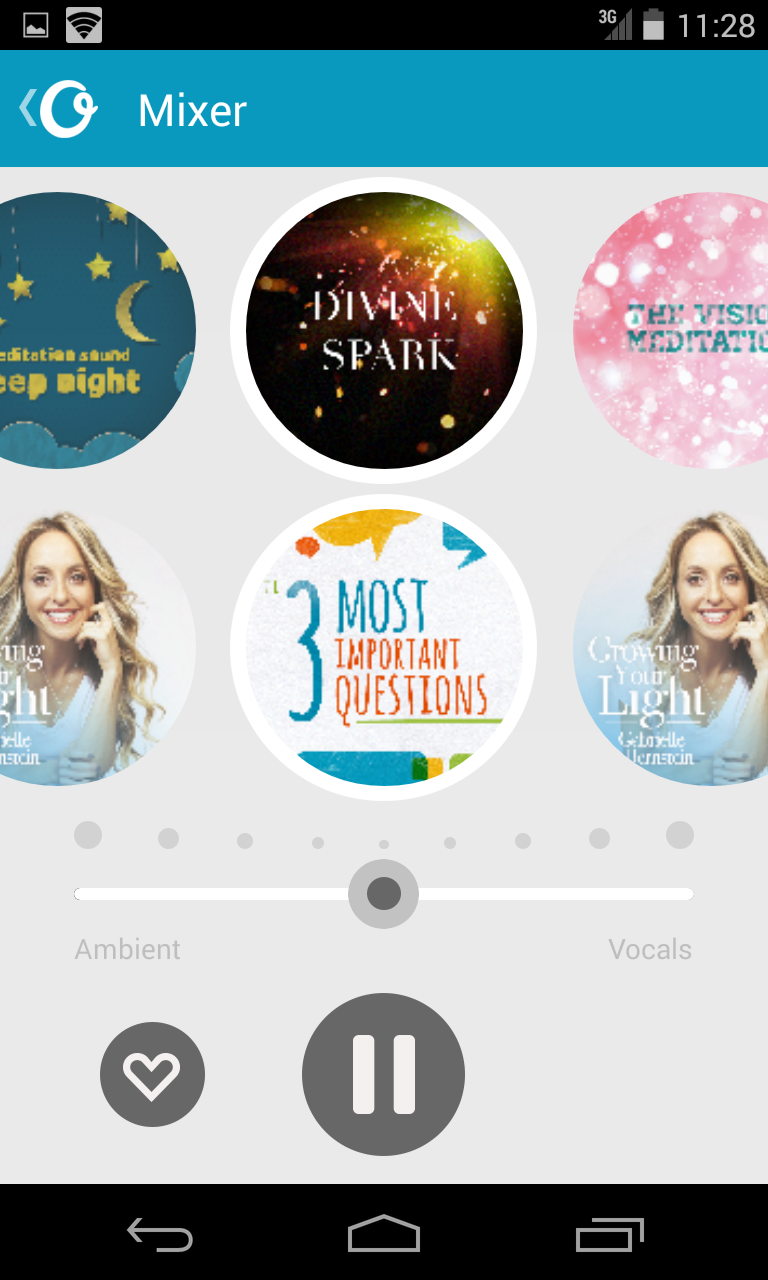
\includegraphics[width=0.45\textwidth]{figures/OMV_mixer_screenshot.png}
\caption{Appearance of the home screen and mixer of the Omvana application.}
\label{fig:OMV_HomeMixerScreens}
\end{figure}

Now we will analyse the store interface. When the user enters the store, he is asked to login using his Facebook account, which will be used to save purchased tracks in case he switches terminals. After a successful login, the Featured page is shown, which offers the user the first selection of content for purchase. The look and feel of the store has been designed to resemble Android's Play Store, with a slider menu that offers the different sections. Different screenshots of the store are shown in figure \ref{fig:OMV_storeScreens}.

\begin{figure}[H]
\centering
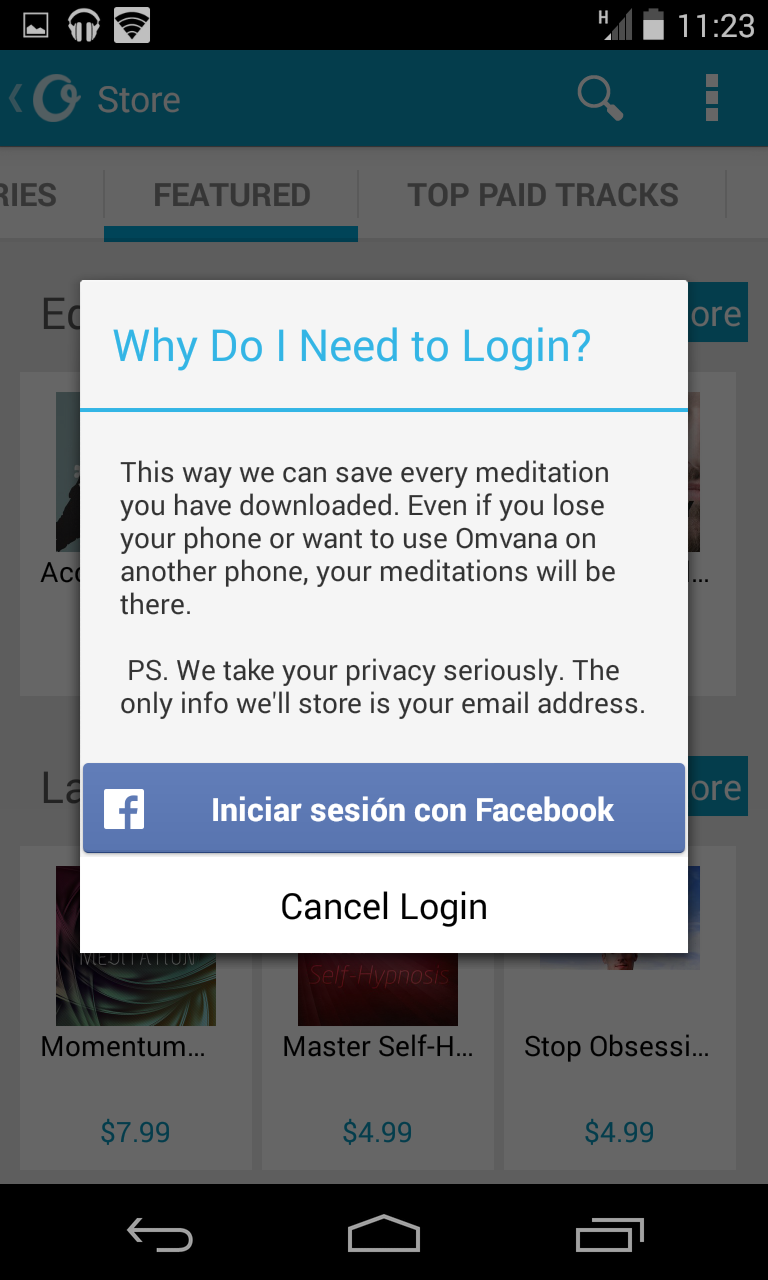
\includegraphics[width=0.24\textwidth]{figures/OMV_login_screenshot.png}
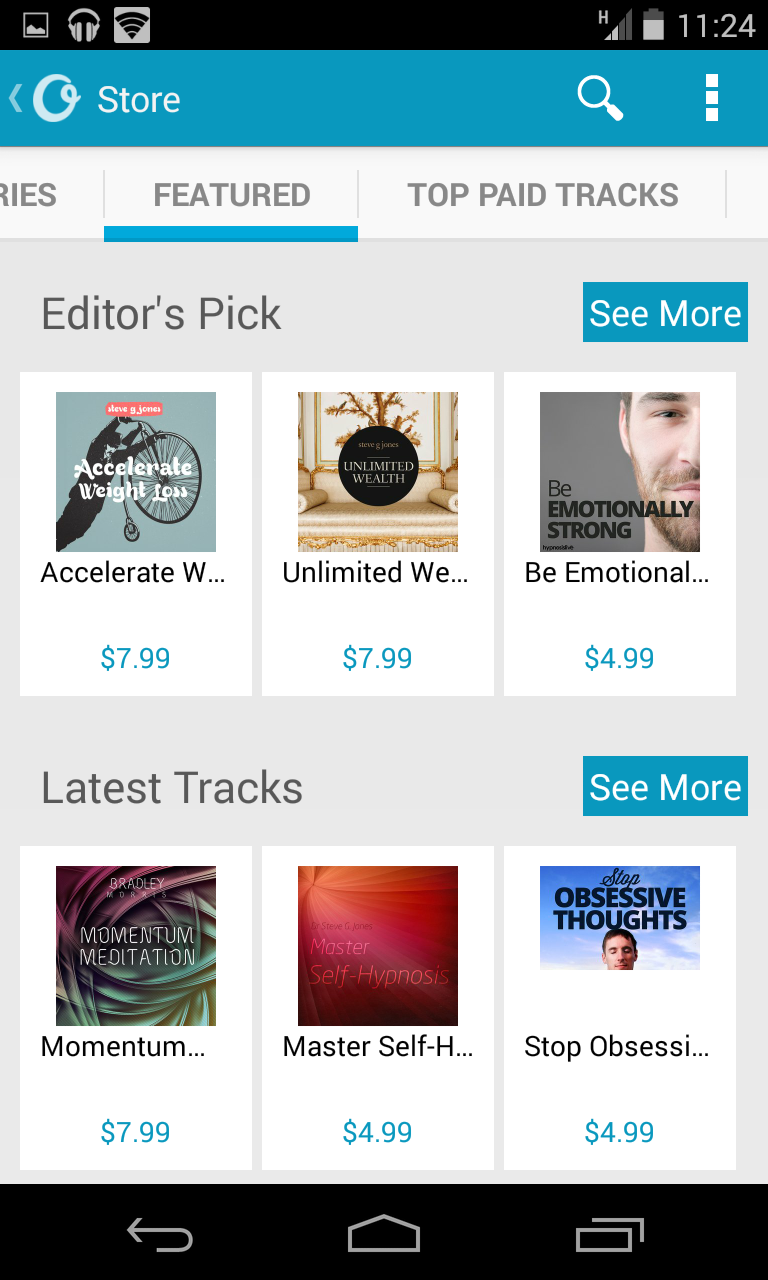
\includegraphics[width=0.24\textwidth]{figures/OMV_store_featured_screenshot.png}
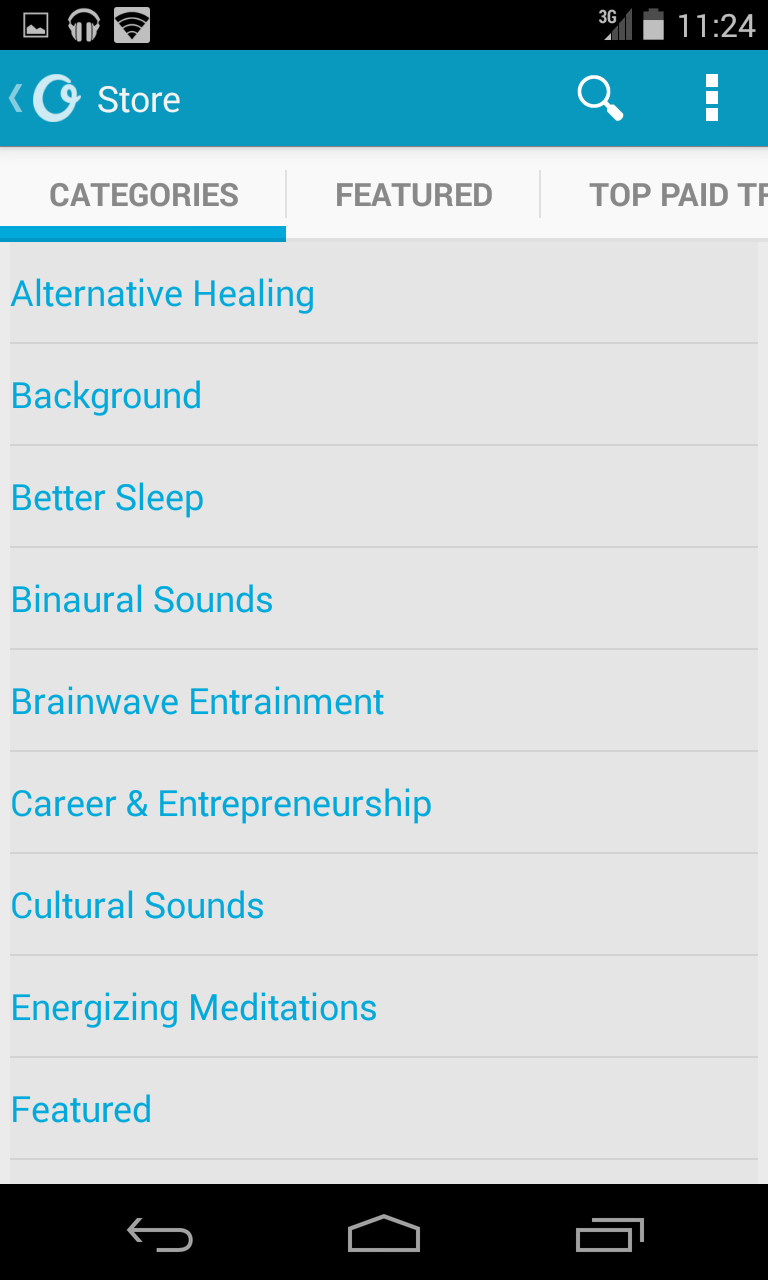
\includegraphics[width=0.24\textwidth]{figures/OMV_store_categories_screenshot.png}
\includegraphics[width=0.24\textwidth]{figures/OMV_store_paid_screenshot.png}
\caption{Appearance of the Omvana store.}
\label{fig:OMV_storeScreens}
\end{figure}

When an item is selected, there is an option to preview a few seconds of the track, which plays it on the same screen. If Download is clicked, a progress bar is shown until the download finishes. Then the button changes to Play, which if clicked goes directly to the player. \\

\begin{figure}[H]
\centering
\includegraphics[width=0.32\textwidth]{figures/OMV_track_page_screenshot.png}
\includegraphics[width=0.32\textwidth]{figures/OMV_preview_item.png}
\includegraphics[width=0.32\textwidth]{figures/OMV_track_download_screenshot.png}
\caption{Appearance of a single track on the Omvana store.}
\label{fig:OMV_storeScreens}
\end{figure}


\subsubsection{Analysis of content}

Omvana puts great effort into content selection. There is an Author Application form in their website, so anything published in the application market has already gone through the company's filter. The offer of content is very wide. The tracks can be of two different kinds:

\begin{itemize}
\item Spoken tracks: Meditations, hypnosis, inspiring talks, motivation speeches...
\item Music tracks: Relaxation music, binaural sounds, nature 
\end{itemize}

There is both paid and free content, available for easy downloading to the users. 

\subsubsection{Analysis of business model and strategy}

Omvana is a content publisher, so they provide the platform for the authors to sell their content. We haven't been able to find the actual numbers, but Mindvalley most likely gets a percentage of every in-app purchase, same as Apple or Google get a cut on their app market's purchases.

\subsubsection{Critical Analysis}

Omvana has been dubbed as "The Spotify of Meditation", and rightfully so, since it tops the charts for Lifestyle applications in more than 30 countries. The whole application has a professional look\&feel, the navigation is seamless and the Store works just as the native Play Store, making it easy for the users to adapt. The mixer is a nice touch, that gives the users another level of customization. The quantity of content is colossal, although quality may vary. It is clear after using this application that there is a big team behind taking care of both the content and the application functionality. 

\subsubsection{Users' feedback}

On Google Play, the application has a 3.5 out of 5 rating with 72 total opinions. The application is so new that still there are no comments.  \\

On iTunes App Store, the application has a 4.5 out of 5 rating with 1626 total opinions. The comments talk about the ways listening to the contents have helped the users coping with problems or improving their lives, but very few discuss the actual application. Some of the features users suggest are:\\

\begin{itemize}
\item A timer to shut off the tracks after a certain time (which is included in sister app Dormio).
\item More flexibility for the mixer, so you can mix two background tracks instead of vocals/background only.
\item Review mechanism for the content, so users can rate the tracks they download.
\end{itemize}

The negative comments are mostly about instability issues, that seems resolved with the last updates. Also with the obligation to use a Facebook account to login to retain in-app purchases.  

\subsubsection{Wrap-up}

This application differs to most of the other ones in that its only role is as a content provider, not generating its own content. This lets them focus on design and usability, providing a very stable and well thought out experience. The biggest drawback of this approach is that on one side you need a large user base which is willing to pay for quality content, and on the other, authors generating this content that are willing to share their profit by using your platform. In this case the company already had both the user base and the authors before launching the application, this way they reached over $300.000$ iOS downloads in less than six months. 

% ----------------------
%        HEADSPACE
% ----------------------

\subsection{Headspace}
\begin{wrapfigure}{l}{0.08\textwidth}
  \vspace*{-0.8cm}
  \begin{center}
    \includegraphics[width=0.08\textwidth]{figures/HS_icon.png}
  \end{center}
  \vspace*{-0.5cm}
\end{wrapfigure}

Headspace is a full meditation platform founded by Andy Puddicombe, a former Buddhist monk turned speaker and published author. The philosophy of Headspace is to apply all the concepts of classic meditation but stripping out any religious or transcendental wrapping that usually go with it. This way they can reach a public that otherwise would be repelled by the yoga positions, incense sticks, zen gardens and in general what could be called ``new age'' look. The project launched initially in 2010 as a web platform, later expanding to the mobile application environment. As of July 2014, the whole platform just underwent a total design and content overhaul.  \\

The application is offered for free, both for Android and iOS, but most of the content is available to subscribers only. The subscription rates are as follows:

\begin{itemize}
\item Monthly: \euro{9,95}
\item Yearly: \euro{71,88} (\euro{5,99}/month)
\item Two years: \euro{113.76} (\euro{4,74}/month)
\item Forever: \euro{395,95}
\end{itemize}

Headspace has been downloaded around $144.000$ times for Android and $227.000$ times for iOS (estimated by xyo.net). \\

The application is not localised, being offered only in the English language. 

\subsubsection{Features} 

The features described by the developer are:

\begin{itemize}
\item Free access to Take10, Level 1 of the Foundation Course. Learn the basics in 10 x 10 minute meditations.
\item Personalised progress page to track your stats.
\item Buddy system for you and your friends to motivate each other in your journey's.
\item Rewards for regular meditation.
\item Reminders to keep you on track with your practice.
\item Options for you to continue your journey after Take10, with inspiring packs and one off sessions on a range of topics such as stress, happiness and appreciation.
\item Ability to download sessions for offline use.
\end{itemize}


\subsubsection{Analysis of the user interface}

We will analyse the Android application, which is the one we have access to. The first time the user opens the application, a six step introduction tour is shown, which can be seen in figures \ref{fig:HS_tourScreens1} y \ref{fig:HS_tourScreens2}.

\begin{figure}[H]
\centering
\includegraphics[width=0.32\textwidth]{figures/HS_tour1_screenshot.png}
\includegraphics[width=0.32\textwidth]{figures/HS_tour2_screenshot.png}
\includegraphics[width=0.32\textwidth]{figures/HS_tour3_screenshot.png}
\caption{Introduction tour for the Headspace application.}
\label{fig:HS_tourScreens1}
\end{figure}

\begin{figure}[H]
\centering
\includegraphics[width=0.32\textwidth]{figures/HS_tour4_screenshot.png}
\includegraphics[width=0.32\textwidth]{figures/HS_tour5_screenshot.png}
\includegraphics[width=0.32\textwidth]{figures/HS_tour6_screenshot.png}
\caption{Introduction tour for the Headspace application.}
\label{fig:HS_tourScreens2}
\end{figure}

After the introduction tour, the main screen is shown, but with a translucent message that instructs on how to navigate through the main application tabs, shown in figure \ref{fig:HS_mainScreens1}. Also every screen has a question mark on the top right that further explains how the application works. This overly guided interface shows a lack of confidence from the designer's point, as if the navigation is not intuitive enough for the average user to grasp without constant guiding. \\

The main screens are Timeline, Progress and Buddies. The Timeline is a visual way of working through each of the meditations, unlocking the next each time one is completed. When a practice is selected, the meditation screen opens. The design is simple, at the top it shows the level, session and time, with a big Play/Pause button in the middle. A nice added touch is that the round button organically changes its shape during the meditation. It is shown in figure \ref{fig:HS_mainScreens1}. \\

The Progress screen shows the user's statistics, such as average practice duration, number of sessions or total time meditating. It also shows the number of users meditating in that moment, strengthening the feeling of community, and finally a simple achievement system that rewards the user for consecutive days meditating. The Buddies section lets the user follow their friends, again trying to give a sense of community. All of them are shown in figure \ref{fig:HS_mainScreens2}.

\begin{figure}[H]
\centering
\includegraphics[width=0.32\textwidth]{figures/HS_main_help_screenshot.png}
\includegraphics[width=0.32\textwidth]{figures/HS_timeline_screenshot.png}
\includegraphics[width=0.32\textwidth]{figures/HS_meditation_screenshot.png}
\caption{Main screens of the Headspace application.}
\label{fig:HS_mainScreens1}
\end{figure}

\begin{figure}[H]
\centering
\includegraphics[width=0.32\textwidth]{figures/HS_progress1_screenshot.png}
\includegraphics[width=0.32\textwidth]{figures/HS_progress2_screenshot.png}
\includegraphics[width=0.32\textwidth]{figures/HS_buddies.png}
\caption{Main screens of the Headspace application.}
\label{fig:HS_mainScreens2}
\end{figure}

In the top right corner, beside the question mark, there are two icons that are hard to understand at first sight. Upon clicking them we learn they give access to more content: the left one is Series and the right one is Singles. The screens for them are shown in figure \ref{fig:HS_singlesSeries}. As can be seen in the last screen, all this content is subscriber only.

\begin{figure}[H]
\centering
\includegraphics[width=0.24\textwidth]{figures/HS_series_screenshot.png}
\includegraphics[width=0.24\textwidth]{figures/HS_singles_screenshot.png}
\includegraphics[width=0.24\textwidth]{figures/HS_singles_sos_screenshot.png}
\includegraphics[width=0.24\textwidth]{figures/HS_singles_subscription_screenshot.png}
\caption{Series and Singles screens of the Headspace application.}
\label{fig:HS_singlesSeries}
\end{figure}

The rest of the application content is accessed using the top left menu button, that on press opens a \emph{Facebook style} side menu. This menu is shown in figure \ref{fig:HS_menuScreens}

\begin{figure}[H]
\centering
\includegraphics[width=0.32\textwidth]{figures/HS_menu1_screenshot.png}
\includegraphics[width=0.32\textwidth]{figures/HS_menu2_screenshot.png}
\caption{Side menu of the Headspace application.}
\label{fig:HS_menuScreens}
\end{figure}

The remaining screens of the application are:

\begin{itemize}
\item Animations: Short videos containing explanations on what mindfulness is and how to approach it.
\item Support: Link to the FAQ on the website.
\item Get more Headspace: What subscription offers and subscription options.
\item The Science: How some studies revealed the benefits of mindfulness on lifestyle, performance, relationships and health.
\item Andy: Brief introduction to the pivotal role in Headspace, Andy Puddicombe.
\item Get some, give some: Corporate Social Responsibility, each subscription is matched with another free to someone in need.
\item Downloads: Lets the user pre-download content for offline access.
\item Set Reminders: Alarm to remember meditating.
\item Set Mindfulness Buzzers: Daily messages to keep the user mindful. Can be set from 1 to 5 a day.
\item Switch to V1: Lets the user access the pre-update content.
\end{itemize}

Some of the more meaningful screens are shown in figures \ref{fig:HS_restScreens1} and \ref{fig:HS_restScreens2}.

\begin{figure}[H]
\centering
\includegraphics[width=0.32\textwidth]{figures/HS_animations_screenshot.png}
\includegraphics[width=0.32\textwidth]{figures/HS_buzzer_screenshot.png}
\includegraphics[width=0.32\textwidth]{figures/HS_downloads_screenshot.png}
\caption{Animation, Mindfulness Buzzer and Download screens of the Headspace application.}
\label{fig:HS_restScreens1}
\end{figure}

\begin{figure}[H]
\centering
\includegraphics[width=0.32\textwidth]{figures/HS_reminder_screenshot.png}
\includegraphics[width=0.32\textwidth]{figures/HS_science_screenshot.png}
\includegraphics[width=0.32\textwidth]{figures/HS_whosandy_screenshot.png}
\caption{Reminder,Science and Who's Andy screens of the Headspace application.}
\label{fig:HS_restScreens2}
\end{figure}


\subsubsection{Analysis of content}

The amount of content this platform offers is astonishing. There are two main blocks: Series and Singles. Series are groups of meditations designed to be practised in order, one at a day. Singles, on the other hand, are designed to be listened in any order and time, when the user feels they could be helpful. \\

The Series content is split in:

\begin{itemize}
\item Foundation: The introduction to meditation and mindfulness. Three 10-day levels which unlock the entire library on completion.
\item Health: Three 30-day packs on Stress, Anxiety and Sleep.
\item Relationships: A 30-day pack on Relationships and two 10-day packs on Change and Appreciation.
\item Performance: Two 30-day packs on Creativity and Focus and a 10-day pack on Happiness.
\item Headspace Pro: Three 10-day levels as an introduction to silent meditation. 
\end{itemize}

The Singles content consists of:

\begin{itemize}
\item SOS: Three two-minute exercises to take the heat off a heated or stressful situation.
\item On-the-go: Meditation applied to everyday activities like sleeping, walking, eating, commuting, cooking and running.
\item Classic: One-off meditation sessions in guided and unguided formats, from 10 to 60 minutes.
\end{itemize}

All the practices are recorded by Andy Puddicombe himself, and are available in the web platform as well. 

\subsubsection{Analysis of business model and strategy}

Headspace is a subscription platform. Only the first 10 practices are free to try, and after that if you want to continue listening to more content you need to pay the monthly, yearly, 2 years or forever subscription. The strategy is to show in only ten days the benefits of meditation to the users who try it, so they become subscribers after that. The company is rumoured to have over 1 million registered users as of now (of course, registered users doesn't mean subscribers). Anyhow, the number of current users meditating shown in the app is always over $3.000$. \\

After such a big visual and technical overhaul, the next step is to probably expand via localization and internationalisation, offering the content in other languages as well. 

\subsubsection{Critical Analysis}

As a full meditation platform, this is probably the most complete and well thought out. The new application and web site are perfectly integrated, with a coherent visual style. The design uses a lot of illustrations that try to give it a more modern look. Everything, from the design, to the text and the actual content, tries to remove the overly transcendental and religious impression that most people have on meditation. \\

It is also obvious that a big part of the success of the platform comes from the man behind it, Andy Puddicombe, which was already working as a meditation teacher and speaker before launching Headspace. His TED Talk on meditation benefits has almost 4 million views, and has been featured widely in international press and on TV. 

\subsubsection{Users' feedback}

On Google Play, the application has a 4.5 out of 5 rating with $6.224$ total opinions. Most of the comments praise the content, and how it is a very good way of getting into meditation. Only one negative comment talks about a bug that we haven't been able to reproduce. \\

On iTunes App Store, the application has a 4 out of 5 rating with 394 total opinions. The comments mostly resemble the ones on Google Play, talking about how a life-changer this application can be and how easy it is to start practising. Some users would prefer a more serious design, but still give it the 5 stars since the important part is the content. 

\subsubsection{Wrap-up}

This application shows that a subscription approach to releasing meditation content is feasible. The most important parts of this approach are giving the user a sense of progress, and regularly releasing new content to put more value into the subscription. \\

Also remarkable is the way in which this application presents meditation without the usual accompanying characteristics like yoga positions, incense sticks and Buddhist symbols. This opens the reach of the application to a much more wider audience.


%--------------------------------------------------------------
%			AEON Mindfulness App
%--------------------------------------------------------------

\subsection{AEON Mindfulness App}
\begin{wrapfigure}{l}{0.08\textwidth}
	\vspace*{-0.8cm}
	\begin{center}
		\includegraphics[width=0.08\textwidth]{figures/AEON_icon.png}
	\end{center}
	\vspace*{-0.5cm}
\end{wrapfigure}
This app has been used to carry out some research about the progress in the mindfulness of some novice meditators in comparison with other two well-known techniques for distancing from thoughts. The authors, L. Chittaro and A. Vianello, claim to prove that AEON allowed participants to reach a better level of mindfulness than traditional methods. Moreover, they claim their app to be more pleasant and easy to practice than traditional methods. This study is gathered in \cite{Chittaro}. 

The app main functionality is an assistant to the user to practice some techniques through which he or she will be able to learn how to maintain control of his or her thoughts, and be able to observe and disolve them, rather than reacting and being completely fullfilled by them.  

AEON is somehow a bit intrusive, as it is needed to accept some terms and conditions to be part of the study as well as to fill a questionaire, which is not short, so the time since the user installs the app until he or she is truly able to use it may be quite long and not user-frienly.


\subsubsection{Features}
The Features text provided in the Google Play Store for the AEON Mindfulness App is reproduced here: "The AEON app helps users in practicing a mindfulness technique that requires individuals not to react in response to their thoughts, but to be aware of them and observe them while they are going away (distancing from thoughts). The effectiveness of the AEON app was tested in a thorough lab study, published by the International Journal of Human-Computer Studies (Elsevier), see http://hcilab.uniud.it/publications/2014-02.html. For more information, visit also the AEON page: http://hcilab.uniud.it/aeon".

\subsubsection{Analysis of the user interface}
Once the two basic questionaries have been answered in the beginning, the AEON Mindfulness App main interface is very simple and meager: two buttons at the top of the screen would allow the user to add and delete new thoughts; at the bottom, the "Info" section is available next to the "Practice" button, which is used to initialize the technique once a thought has been selected among the list. Once a thought has been selected, a brief tutorial on how to perform the technique is displayed. At this moment, the user is prompted to tap repeatedly on the screen, producing a wave effect which will make the text containig the thought dissapear eventually. Once the text has completely dissapeared, indications on how to go to the next thought or to return to the main screen are displayed. All the functionalities described are shown, in order, in figure \ref{fig:AEON_Main_interface}

\begin{figure}[H]
\centering
\includegraphics[width=0.24\textwidth]{figures/AEON_Main_interface_list.png}
\includegraphics[width=0.24\textwidth]{figures/AEON_Practice_01.png}
\includegraphics[width=0.24\textwidth]{figures/AEON_Practice_02.png}\\
\includegraphics[width=0.24\textwidth]{figures/AEON_Practice_03.png}
\includegraphics[width=0.24\textwidth]{figures/AEON_Practice_04.png}
\caption{AEON Mindfulness App main interface and operation.}
\label{fig:AEON_Main_interface}
\end{figure}

Although it is quite simple, the user interface is meager and limited, and not fancy in its desing. All main screens and buttons are displayed in different tones of blue, with a small drawing of a plant in the background; the button's design is very squared, and the text font does not seem appropiate. 

Figures \ref{fig:AEON_Intro_Questionnaire} and \ref{fig:AEON_Mind_Questionnaire} gather the screenshots of the introduction and mindfulness quiestionnaire, respectively. 

\begin{figure}[H]
\centering
\includegraphics[width=0.20\textwidth]{figures/AEON_Intro_01.png}
\includegraphics[width=0.20\textwidth]{figures/AEON_Intro_02.png}
\includegraphics[width=0.20\textwidth]{figures/AEON_Intro_Quest_01.png}
\includegraphics[width=0.20\textwidth]{figures/AEON_Intro_Quest_02.png}
\caption{AEON Mindfulness App introduction questionnaire.}
\label{fig:AEON_Intro_Questionnaire}
\end{figure}

\begin{figure}[H]
\centering
\includegraphics[width=0.20\textwidth]{figures/AEON_Mind_Quest_01.png}
\includegraphics[width=0.20\textwidth]{figures/AEON_Mind_Quest_02.png}
\includegraphics[width=0.20\textwidth]{figures/AEON_Mind_Quest_03.png}
\includegraphics[width=0.20\textwidth]{figures/AEON_Mind_Quest_04.png}
\includegraphics[width=0.20\textwidth]{figures/AEON_Mind_Quest_05.png}
\includegraphics[width=0.20\textwidth]{figures/AEON_Mind_Quest_06.png}
\caption{AEON Mindfulness App mindfulness questionnaire.}
\label{fig:AEON_Mind_Questionnaire}
\end{figure}

Finally, the "Info" section contains the following:

\begin{itemize}
\item Tutorial: if this option is selected, the tutorial is repeated.
\item About: information about the objective and contribution of the app.
\item Temrs and conditions: legal terms and conditions to use the app.
\item Send feedback: a textbox is displayed to allow the user to contribute with some feedback for the authors. 
\end{itemize}

The displayed tutorial is as in figure \ref{fig:AEON_Tutorial}.

\begin{figure}[H]
\centering
\includegraphics[width=0.24\textwidth]{figures/AEON_Tutorial_01.png}
\includegraphics[width=0.24\textwidth]{figures/AEON_Tutorial_02.png}
\caption{AEON Mindfulness App tutorial.}
\label{fig:AEON_Tutorial}
\end{figure}

\subsubsection{Analysis of content}
The content of this app is very limited, but it is according with its functionalities. The purpose of this software is to be part of a scientific research related to the management of thougths and the stated of mindfulness of some novice meditation practicioners. However, from a broader mindfulness point of view, the content of this app is scarce. 

\subsubsection{Analysis of business model and strategy}
As the use of this app is focused on contributing to a scientifical research, it is free to download and has no in-app purchases; so, it is not bussiness-oriented and the authors intend to make no profit with it.

\subsubsection{Critical Analysis}
As it has been previously mentioned, from a wide mindfulness point of view, this app is scarce in content and very limited in usage. It could be of some help when dealing with some specific therapies oriented to thoughts control; however, no other meditation or mindfulness practices can be accomplished with this app.

\subsubsection{Users' feedback}
The Android version of this app has been rated 3.8 stars over 5, by july 17th 2014. Only 22 users have rated the app, which is a very low number and the puntuation is not statistically significant. No text opinions are available at the Google Play Store. 

\subsubsection{Wrap-up} 
In general, this app is research oriented, and thus its content is very scarce and limited, and does not seem very interesting for people seeking for mindfulness and meditation oriented apps. 


%--------------------------------------------------------------
%			BUDDHIST MEDITATION TRAINER
%--------------------------------------------------------------

\subsection{Buddhist meditation trainer}
\begin{wrapfigure}{l}{0.08\textwidth}
	\vspace*{-0.8cm}
	\begin{center}
		\includegraphics[width=0.08\textwidth]{figures/BMT_icon.png}
	\end{center}
	\vspace*{-0.5cm}
\end{wrapfigure}
This app is very simple and is comprised only by three different screens: the main screen, the meditation screen and the options screen.

The main screen, which is the left most screenshot in figure \ref{fig:BMT_MainAndMed}, only allows the user to tap on it to begin a meditation. Each meditation screen shows a text and an image of buddhist content, while a time counter indicates the remaining time of meditation. There are two buttons in this screen:

\begin{itemize}
\item Plane icon button: this button makes the application to crash.
\item Speaker icon button: this button allows the user to change the sound options:
\begin{itemize}
\item Silent meditation.
\item Sound at the end of the meditation.
\item Sound during meditation. 
\end{itemize}
\end{itemize}

Each time a meditation is acomplished, a progress bar is increased certain amount; and each time a progress bar is fulfilled, the user meditation level is increased, and so is the meditation time. This level increase can be seen at the right most screenshot of figure \ref{fig:BMT_MainAndMed}.

\begin{figure}[H]
\centering
\includegraphics[width=0.24\textwidth]{figures/BMT_Main.png}
\includegraphics[width=0.24\textwidth]{figures/BMT_Meditation_01.png}
\includegraphics[width=0.24\textwidth]{figures/BMT_Meditation_02.png}\\
\includegraphics[width=0.24\textwidth]{figures/BMT_Meditation_03.png}
\includegraphics[width=0.24\textwidth]{figures/BMT_NextLevel.png}
\caption{Buddhist Meditation Tutorial main screen and several meditation screens.}
\label{fig:BMT_MainAndMed}
\end{figure}

\subsubsection{Features}
The text from the Google Play site describing this app features is as follows:
\begin{itemize}
\item Buddhist Meditation Trainer is your personal trainer for relaxing and enlightening meditation. It features 10 levels of enlightenment with deeper quotes to meditate on in every level. All with a simple to use meditation timer.
Simply start meditating for 5 minutes everyday to feel the difference. After ten days you will gain a level and further enlightenment.
\item You can easily set the meditation sounds and target duration in the preferences screen.
\item Buddhist Meditation Trainer helps you remember to meditate with a daily notification. You can turn this off or on in the configuration page.
\end{itemize}

\subsubsection{Analysis of the user interface}
The user interface is scarce, barely neat and not very well designed. The icons and text displayed in the meditations screens are not well integrated in the app interface, and provide a "patched" overall look. Moreover, some buttons do not work properly and provoke the app to crash.

The "Settings" section, which is displayed in figure \ref{fig:BMT_Settings}, allows the following configuration:

\begin{itemize}
\item Play Meditation Sounds: a three options ratio button allows to choose between:
\begin{itemize}
\item Never play sounds.
\item Plan end sound.
\item Play meditation sounds.
\end{itemize}
\item Meditation sound: a four options ratio button allows to choose between:
\begin{itemize}
\item Burmese Gong.
\item Chinese Gong.
\item Chinese Hand Bell.
\item Zen Bell.
\end{itemize}
\item Max meditation duration: a five options ratio button allows to choose the maximum time of meditation when the maximum level is reached. This option will also affect the duration of meditations' length at each single level. The options are:
\begin{itemize}
\item 15 minutes.
\item 20 minutes.
\item 30 minutes.
\item 40 minutes.
\item 50 minutes.
\end{itemize}
\item Meditation reminder: a three options ratio button which allows to choose between:
\begin{itemize}
\item Off.
\item Every day.
\item Every other day.
\end{itemize}
\end{itemize}

\begin{figure}[H]
\centering
\includegraphics[width=0.24\textwidth]{figures/BMT_Options.png}
\caption{Buddhist Meditation Tutorial Settings screen.}
\label{fig:BMT_Settings}
\end{figure}

\subsubsection{Analysis of content}
The Buddhist Meditation Trainer App only permits to do silent or sound-accompanied meditations, allowing the user to increase his meditation level and so, the meditation duration. Only meditations duration and enviromental sounds can be configured, so the usage of this app is very limited. 

\subsubsection{Analysis of business model and strategy}
The Android version of this app is free to download and has no in-app purchases; so, it is not business-oriented and the authors intend to make no profit with it.

\subsubsection{Critical Analysis}
This app seems appropriate for users which have some experience in meditation techniques, so they are able to perform silent meditations by their own, and have no need or do not want to practice guided ones. Considering this, the only added value this app has over a normal timer to meditate is the possibility to configure in-meditation sounds, and the will of the user to increase his meditation level and, thus, the meditation time. 

\subsubsection{Users' feedback}
This app has a valoration of 4.6 stars over 5, with more than 14.000 votes from the users. By july 17th 2014, it has only 920 votes with 3 stars or below, which is only a 6.26\% of all valorations; that means 93.74\% of users scoring this app with 4 or 5 stars. Most textual valorations mention the fact that this app allows the user to increase his "meditation level", considering it a good stimulus for further progress. 

\subsubsection{Wrap-up} 
Although initially this app seems to be scarce and limited in its content, it is very well valued by the users, which indicates the little content it has is very appropriate from a MBMA point of view. 

%--------------------------------------------------------------
%						BREATHE 2 RELAX
%--------------------------------------------------------------
\subsection{Breathe 2 relax}
\subsubsection{Features}
\subsubsection{Analysis of the user interface}
\subsubsection{Analysis of content}
\subsubsection{Analysis of business model and strategy}
\subsubsection{Critical Analysis}
\subsubsection{User's feedback}
\subsubsection{Wrap-up}


%--------------------------------------------------------------
%			BIBLIOGRAPHY
%--------------------------------------------------------------
\cleardoublepage

\bibliographystyle{unsrt}

\bibliography{refs}

%----------------------------------------------------------------------------------------

\end{document} 